\documentclass[%
	11pt,
	a4paper,
	utf8,
	%twocolumn
		]{article}	

\usepackage{style_packages/podvoyskiy_article_extended}


\begin{document}
\title{Заметки по машинному обучению и анализу данных. Том 2}

\author{\itshape Подвойский А.О.}

\date{}
\maketitle

\thispagestyle{fancy}

Здесь приводятся заметки по некоторым вопросам, касающимся машинного обучения, анализа данных, программирования на языках \texttt{Python}, \texttt{R} и прочим сопряженным вопросам так или иначе, затрагивающим работу с данными.


\shorttableofcontents{Краткое содержание}{1}

\tableofcontents

\section{MAE vs MSE. Устойчивость среднеабсолютной ошибки к выбросам}

Средняя абсолютная ошибка более устойчива к выбросам по сравнению с квадратической ошибкой. Потому что, оптимальным решением на классе константных алгоритмов для квадратической ошибки MSE является \emph{среднее арифметическое}, а для среднеабсолютной MAE -- \emph{медиана}.

Медиана, как известно, является более устойчивой к выбросам по сравнению со средним арифметическим. Несмотря на это, MSE обладает своими достоинствами -- в частности, для нее можно выписать аналитическое решение в случае линейной регрессии, а также ее можно оптимизировать напрямую при помощи градиентного спуска, в отличие от MAE, которая не является дифференциируемой по $ w $. 

\section{Оптимизационные задачи и теорема Куна-Таккера}

Рассмотрим задачу минимизации
\begin{align}\label{eq:opt_task}
\begin{cases}
	f_0 (x) \rightarrow \min\limits_{ x \in \mathbb{R}^d }\\
	f_i(x) \leqslant 0, \ i = 1, \ldots, m,\\
	h_i(x) = 0, \ i = 1, \ldots, p.
\end{cases}
\end{align}

Если ограничения в этой задаче отсутствуют, то имеет место \emph{необходимое условие экстремума}: если в точке $ x $ функция $ f_0 $  достигает своего минимума, то ее градиент в этой точке равен нулю. Значит, для решения задачи \emph{безусловной оптимизации} (нет ограничений)
\begin{align*}
	f_0(x) \rightarrow \min
\end{align*}
достаточно найти все решения уравнения
\begin{align*}
	\nabla f_0(x) = 0,
\end{align*}
и выбрать то, в котором достигается наименьшее значение. Для решения \emph{условных} задач оптимизации (в них есть ограничения) требуется более сложный подход.

Для задачи \eqref{eq:opt_task} можно записать \emph{лагранжиан} (функцию Лагранжа)
\begin{align*}
	L(x, \lambda, \nu) = f_0(x) + \sum_{i=1}^{m} \lambda_i f_i(x) + \sum_{i=1}^{p} \nu_i h_i(x), \ \lambda_i \geqslant 0,
\end{align*}
где $ \lambda_i, \nu_i $ -- \emph{множители Лагранжа} (двойственные переменные).

\emph{Двойственной функцией} для задачи \eqref{eq:opt_task} называется функция, получающаяся при взятии минимума лагранжиана по $ x $
\begin{align*}
	g(\lambda, \nu) = \inf_x L(x, \lambda, \nu).
\end{align*}

Двойственная функция дает \emph{нижнюю оценку} на \underline{минимум} в исходной оптимизационной задаче.

\emph{Условия Каруша-Куна-Таккера} (необходимые условия экстремума)
\begin{align*}
	\nabla f_0(x_*) + \sum_{i=1}^{m} \lambda_i^* \nabla f_i(x_*) + \sum_{i=1}^{p} \nu_i^* \nabla h_i (x_*) = 0\\
	f_i(x_*) \leqslant 0, \ i = 1, \ldots, m\\
	h_i(x_*) = 0, \ i = 1, \ldots, p\\
	\lambda_i^* \geqslant 0, \ i = 1, \ldots, m\\
	\lambda_i^* f_i(x_*) = 0, \ i = 1, \ldots, m
\end{align*}

Если задача \eqref{eq:opt_task} является выпуклой и удовлетворяет условию Слейтера, то условия Куна-Таккера становятся \emph{необходимыми} и \emph{достаточными}.


\section{Векторное дифференциирование}

Иногда при взятии производных по вектору или от вектор-функции удобно оперировать матричными операциями. Это упрощает запись и упрощает вывод формул.

Введем следующие определения:
\begin{itemize}
	\item При отображении вектора в число $ f(x): \mathbb{R}^n \rightarrow \mathbb{R} $ (то есть когда нужно взять производную от скалярной функции векторного аргумента $ f(x_1, \ldots, x_n) $ по каждому аргументу $ x_i $ в отдельности)
\begin{align*}
	\nabla_x f(x) = \Big[ \, \dfrac{ \partial f }{\partial x_1}, \ldots, \dfrac{ \partial f }{ \partial x_n } \, \Big]^T,
\end{align*}

    \item При отображении матрицы в число $ f(A): \mathbb{R}^{n \times m} \rightarrow \mathbb{R} $ (когда нужно взять производную функции от матрицы $ A $ по всем элементам матрицы $ A_{ij} $)
\begin{align*}
	\nabla_A f(A) = \Big( \dfrac{ \partial f }{ \partial A_{ij} } \Big)_{i, j = 1}^{n, m}.
\end{align*}
\end{itemize}

Мы хотим оценить, как функция изменяется по каждому из аргументов по отдельности. Поэтому производной от скалярной функции векторного аргумента по вектору будет \emph{вектор}, по матрице -- \emph{матрица}.

\remark{
Когда говорят, что нужно взять производную от скалярной функции векторного аргумента $ f(\underbrace{x_1, \ldots, x_n}_x) $ по вектору $ x $, это означает, что нужно взять производную от скалярной функции векторного аргумента $ f(x) $ по каждому элементу вектора $ x_i $. То есть запись $ \nabla_x f(x_1, \ldots, x_n) $ означает, частные производные $ \dfrac{\partial}{\partial x_i} $ от $ f(x) $. И аналогично, когда говорят, что нужно взять производную от функции матричного аргумента по матрице, это означает, что нужно взять производную функции матричного аргумента по каждому элементу матрицы. То есть запись $ \nabla_A f(A)$ означает частные производные по каждому элементу матрицы $ \dfrac{ \partial }{ \partial A_{ij} } $ от $ f(A) $
}

\emph{Задача 1}. Пусть $ a \in \mathbb{R}^n $ -- вектор параметров, а $ x \in \mathbb{R}^n $ -- вектор переменных. Необходимо найти производную их скалярного произведения по \emph{вектору переменных} $ \nabla_x a^T x $.

Так как $ a^T x $ это просто линейная комбинация переменных
\begin{align*}
	\dfrac{ \partial }{ \partial x_i } a^T x = \dfrac{ \partial }{ \partial x_i } \sum_j a_j x_j = a_i = \dfrac{ \partial f }{\partial x_i},
\end{align*}
то, собрав все $ n $ компонент $ \dfrac{ \partial f }{ \partial x_i } $ вместе, получим $ \nabla_x \underbrace{a^T x}_{f(x_1, \ldots, x_n)} = a $. То есть результатом будет вектор параметров $ a $.

Заметим, что $ a^T x $ -- это число, поэтому $ a^T x = (a^T x)^T = x^T a $, следовательно $\boxed{\nabla_x x^T a = \nabla_x a^T x = a} $.

\vspace*{3mm}\emph{Задача 2}. Пусть теперь $ A \in \mathbb{R}^{n \times n} $. Необходимо найти $ \nabla_x x^T A x $.
\begin{multline*}
	\dfrac{ \partial }{ \partial x_i } x^T A x = \dfrac{ \partial }{ \partial x_i } \sum_{j} x_j (A x)_j = \dfrac{ \partial }{ \partial x_i} \sum_{j} x_j \Big( \sum_k a_{jk} x_k \Big) = \dfrac{ \partial }{ \partial x_i } \sum_{j,k} a_{jk} x_j x_k = \\
	= \sum_{j \neq i} a_{ji} x_j + \sum_{k \neq i} a_{ik} x_k + 2 a_{ii} x_i = \sum_j a_{ji} x_j + \sum_k a_{ik} x_k = \sum_j (a_{ji} + a_{ij}) x_j.
\end{multline*}

Поэтому $ \boxed{\nabla_x x^T A x = (A + A^T) x} $.

\vspace*{3mm}\emph{Задача 3}. Пусть $ A \in \mathbb{R}^{n \times n} $. Необходимо найти $ \nabla_A \det A $. Воспользуемся теоремой Лапласа о разложении определителя по строке
\begin{align*}
	\dfrac{ \partial }{ \partial A_{\color{red}ij} } \det A = \dfrac{ \partial }{ \partial A_{ij} } \Big[ \sum_k (-1)^{i + k} A_{ik} M_{ik} \Big] = (-1)^{i + j} M_{\color{red}ij},
\end{align*}
где $ M_{ik} $ -- дополнительный минор\footnote{Дополнительным минором $ M_{ij} $ элемента $ a_{ij} $ называется определитель порядка $ n - 1 $, полученный из матрицы $ A $ порядка $ n $ вычеркиванием $ i $-ой строки и $ j $-ого столбца} матрицы $ A $. 

Элементы обратной матрицы
\begin{align*}
	(A^{-1})_{\color{red}ij} = \dfrac{1}{ \det A } (-1)^{i + j} M_{\color{red}ji}.
\end{align*}

Подставляя выражение для дополнительног минора, получаем ответ
\begin{align*}
	\boxed{\nabla_A \det A = (\det A) A^{-T}}
\end{align*}

Действительно, так как $ \det A (A^{-T})_{\color{red}ij}  = (-1)^{i + j} M_{\color{red}ij} $, то $ \dfrac{ \partial }{ \partial A_{ij} } \det A = \det A (A^{-T})_{ij} $.

\vspace*{3mm}\emph{Задача 4}. Пусть $ A \in \mathbb{R}^{n \times n}, B \in \mathbb{R}^{n \times n} $. Необходимо найти $ \nabla_A \text{tr} (AB) $.
\begin{align*}
	\dfrac{ \partial }{ \partial A_{ij} } \text{tr} (AB)  = \dfrac{ \partial }{ \partial A_{ij} } \sum_k (AB)_{kk} = \dfrac{ \partial }{ \partial A_{ij} } = \sum_{k,l} A_{kl}B_{lk} = B_{ji}.
\end{align*}

То есть $ \boxed{\nabla_A \text{tr} (AB) = B^T} $.

\vspace*{3mm}\emph{Задача 5}. Пусть $ x \in \mathbb{R}^n, A \in \mathbb{R}^{n \times m}, y \in \mathbb{R}^m $. Необходимо найти $ \nabla_A x^T A y $. Воспользоваться циклическим свойством следа матрицы (для матриц подходящего размера)
\begin{align*}
	\text{tr} (ABC) = \text{tr} (BCA) = \text{tr} (CAB)
\end{align*}
и результатом предыдущей задачи, получаем
\begin{align*}
	\nabla_A \underbrace{x^T A y}_{(1 \times 1)} = \nabla_A \text{tr} (x^T A y) = \nabla_A \text{tr} \big(  A \underbrace{(y x^T)}_B \big) = B^T = xy^T.
\end{align*}

\subsection{Решение задачи регрессии для многомерного случая}

В общем случае мы имеем выборку $ \{ (x_i, y_i)_{i=1}^l \},\ x_i \in \mathbb{R}^d, \ y \in \mathbb{R}, \ i = (1, \ldots, l) $ и мы хотим найти наилучшие парамемтры модели $ a(x) =  \langle w, x \rangle $ с точки зрения минимизации функции ошибки (то есть с точки зрения квадратической функции потерь)
\begin{align*}
	Q(w) = (y - X w)^T (y - X w).
\end{align*}

Здесь $ X \in \mathbb{R}^{l \times d} $ -- матрица <<объекты-признаки>> для обучающей выборки, $ y \in \mathbb{R}^l $ -- вектор значений целевой переменной на обучающей выборке, $ w \in \mathbb{R}^d $ -- вектор параметров.

Выпишем градиент функции ошибки по $ w $ (это просто скалярная функция векторного аргумента)
\begin{align*}
	\nabla_w Q(w) = \nabla_w [\, y^T y - y^T X w - w^T X^T y + w^T X^T X w \,] = 0 - X^T y - X^T y + (X^T X + X^T X) w = 0.
\end{align*}

Рассмотрим подробнее второй элемент в квадратных скобках $ \nabla_w \big(\underbrace{y^T}_{(1 \times l)} \underbrace{X}_{( l \times d )} \underbrace{w}_{( d \times 1)} \big) = \nabla_w \big( \underbrace{y^T X}_{(1 \times d)} \underbrace{w}_{( d \times 1)} \big) $. То есть в обозначениях $ \nabla_x a^T x = a $, $ y^T X = a^T $, а $ w = x $. Следовательно, здесь $ a = (y^T X)^T = X^T y $.

Аналогично для третьего элемента $ \nabla_w \big( w^T X^T y \big) $ в терминах $ \nabla_x x^T a = a $, элемент $ w^T = x^T $, а элемент $ X^T y = a $. То есть решением будет просто $ a = X^T y $.

Для четвертого элемента следует использовать формулу $ \nabla_x x^T A x = (A + A^T) x $.

Таким образом, искомый вектор параметров выражается так
\begin{align*}
	w = (X^T X)^{-1} X^T y.
\end{align*}

Покажем, что найденная точка -- точка минимума, если матрица $ X^T X $ обратима. Из курса матана мы знаем, что если матрица Гессе функции положительно определена в точке, градиент которой равен нулю, то эта точка является локальным минимумом (достаточное условие существования экстремума)

\begin{align*}
	\nabla_w^2 Q(w) = \nabla_w \big( 2X^T X\,w \big) = 2 X^T X \, \nabla_w w = \underbrace{2 X^T X}_{( d \times d )} \, \underbrace{E}_{(d \times d)} = 2 X^T X.
\end{align*}

Так как числовую матрицу соответствующих размеров можно выносить за знак производной.

Необходимо понять является ли матрица $ X^T X $ положительно определенной. Запишем определение положительной определенности матрицы $ X^T X $
\begin{align*}
	z^T X^T X z > 0, \forall z \in \mathbb{R}^d, \ z \neq 0.
\end{align*}

Видим, что тут записан квадрат нормы вектора $ X z $, то есть $ \| X z \|^2 \geqslant 0 $. В случае, если матрица $ X $ имеет книжную ориентацию (строк не меньше, чем столбцов) и имеет \emph{полный ранг}\footnote{Говорят, что у матрицы $ A \in \mathbb{R}^{n \times m} $ полный ранг, если $ \text{rg} A = \min(n, m) $} (нет линейно зависимых столбцов), то вектор $ X z $ не может быть нулевым, а значит выполняется
\begin{align*}
	z^T X^T X z = \| X z \|^2 > 0, \forall z \in \mathbb{R}^d, z \neq 0.
\end{align*}

Ранг матрицы равен наибольшему порядку отличного от нуля минора этой матрицы. 

То есть $ X^T X $ является положительно определенной матрицей. Если же строк оказывается меньше, чем столбцов, или $ X $ не является полноранговой (есть линейно зависимые столбцы), то $ X^T X $ \emph{необратима} ($ \det X^T X = 0 $) и решение $ w $ определено \emph{неоднозначно}.

\subsection{Градиентный спуск}

Ситуация, когда нам удается найти решение оптимизационной задачи в явном виде, -- большая удача. В общем случае оптимизационные задачи можно решать \emph{итерационно} с помощью \emph{градиентных методов} (или же методов, использующих как градиент, так и информацию о производных более высокого порядка).

\emph{Антиградиент} $ (- \nabla f(x_1, \ldots, x_n)) $ является направлением наискорейшего \underline{убывания} функции в заданной точке.

\section{Классические алгоритмы машинного обучения}

\subsection{Линейная регрессия}

Дано: коллекция размеченных данных $ \{ \mathbf{x}_i, y_i \}_{i=1}^N $, где $ N $ -- размер коллекции, $ \mathbf{x}_i $ -- D-мерный вектор признаков образца $ i = 1, \ldots, N $, $ y_i $ -- действительное целевое значение, и каждый признак $ x_i^{(j)}, j = 1, \ldots, D $ также является действительным числом.

Требуется: сконструировать модель $ f_\mathbf{w}, b (\mathbf{x}) $, являющуюся \emph{линейной комбинацией признаков экземпляра} $ \mathbf{x} $
\begin{align*}
	f_{ \mathbf{w}, b } (\mathbf{x})  = \mathbf{w} \mathbf{x} + b,
\end{align*}
где $ \mathbf{w} $ -- $ D $-мерный вектор параметров, $ b $ -- действительное число (смещение).

Запись $ f_{\mathbf{w}, b} $ означает, что модель параметризуется двумя значениями: $ \mathbf{w} $ и $ b $.

В линейной регрессии, в отличие от метода опорных векторов, \emph{гиперплоскость} проводится так, чтобы оказаться как можно ближе ко всем \emph{обучающим образцам}.

Чтобы удовлетворить это последнее требование (о прохождении гиперплоскости как можно ближе ко всем обучающим образцам), процедура оптимизации, используемая для поиска оптимальных значений $ \mathbf{x}^{*} $ и $ b^{*} $, должна \emph{минимизировать} следующее выражение \cite[\strbook{44}]{burkov:2020}
\begin{align*}
	\dfrac{1}{N} \sum_{i=1}^N \big( f_{\mathbf{w}, b} (\mathbf{x}_i) - y_i \big)^2.
\end{align*}

\remark{
Вместо квадартической функции потерь можно было использовать и функцию абсолютного отклонения, но последняя в отличие от квадратической функции потерь \emph{негладкая} (т.е. не имеет непрерывной производной) и потому создает лишние сложности, когда для поиска аналитических решений оптимизационных задач используются методы линейной алгебры.
}

Аналитические решения для нахождения оптимума функции -- это простые алгебраические выражения, и они часто предпочтительнее использования сложных \emph{численных методов оптимизации}, таких как \emph{градиентный спуск}.

Очевидно, что квадраты штрафов выгодны еще и потому, что преувеличивают разность между истинными и прогнозируемыми целевыми значениями, в соответствии с величиной этой разности.

\subsection{Логистическая регрессия}

Модель логистической регрессии
\begin{align*}
	f_{ \mathbf{w}, b } (\mathbf{x}) \mathrel{\stackrel{\rm def}=} \dfrac{1}{ 1 + e^{-( \mathbf{w} \mathbf{x} + b )} }
\end{align*}

То есть другими словами модель логистической регрессии представляет собой линейную комбинацию признаков, обернутую \emph{логистическим сигмоидом} $ \sigma(x) $, т.е.
$$
f_{ \mathbf{w}, b } (\mathbf{x}) = \sigma \Bigg( \sum_{i=1}^{N} w_i x_i + b \Bigg), \quad \sigma(x) = \dfrac{1}{ 1 + e^{-x} }.
$$

\remark{
В \emph{линейной регрессии} \underline{минимизируется} средне квадратическая ошибка (MSE), а в \emph{логистической регрессии} \underline{максимизируется} \emph{логарифм функции правдоподобия}
}

В статистике функция правдоподобия определяет, насколько правдоподобным выглядит наблюдение (образец) в соответствии с нашей моделью \cite[\strbook{48}]{burkov:2020}.

Критерий оптимизации в логистической регрессии называется максимальным правдоподобием. Вместо того чтобы минимизировать среднеквадратическую ошибку, как в линейной регрессии, мы теперь максимизируем правдоподобие обучающих данных в соотвествии с моделью
\begin{align*}
	L_{ \mathbf{w}, b } \mathrel{ \stackrel{\rm def} = } \prod_{i=1}^{N} f_{ \mathbf{w}, b } (\mathbf{x}_i)^{y_i} \, \big( 1 - f_{ \mathbf{w},b } (\mathbf{x}_i) \big)^{ (1 - y_i) }.
\end{align*}

Выражение $ f_{ \mathbf{w}, b } (\mathbf{x}_i)^{y_i} \, \big( 1 - f_{ \mathbf{w},b } (\mathbf{x}_i) \big)^{ (1 - y_i) } $ всего навсего означает, что <<$ f_{ \mathbf{w}, b } (\mathbf{x}_i) $, когда $ y_i = 1 $, и $ (1 - f_{ \mathbf{w},b } (\mathbf{x}_i)) $ иначе>>.

Таким образом, задача оптимизации в случае логистической регрессии имеет вид
\begin{align*}
	\argmin_{ \mathbf{w}, b } - \sum_{i=1}^N \Big[ y_i \ln f_{ \mathbf{w}, b } (\mathbf{x}) + (1 - y_i) \ln \big( 1 - f_{ \mathbf{w}, b } (\mathbf{x}_i) \big) \Big].
\end{align*}

В отличие от линейной регрессии, задача оптимизации выше не имеет аналитического решения. Поэтому в таких случаях обычно используется процедура численной оптимизации -- градиентный спуск.

\subsection{Деревья решений}

Дерево решений -- это ациклический граф, который можно использовать для принятия решений. В каждом ветвящемся узле графа исследуется $ j $-ый признак из вектор признаков. Если значение признака ниже определенного порога, то выбирается левая ветвь, а иначе -- правая. По достижении листового узла принимается решение о классе, к которому принадлежит образец.

В алгоритме \emph{ID3} качество расщипления оценивается с использованием энтропии. Энтропия достигает своего минимума, когда случайная величина может иметь только одно значение. И достигает своего максимума, когда все значения случайной величины равновероятны.

Алгоритм ID3 останавливается на листовом узле в любой из следующих ситуаций:
\begin{itemize}
	\item Все примеры в листовом узле правильно классифицируются моделью,
	
	\item Невозможно найти атрибут для расщипления,
	
	\item Расщипление уменьшает энтропию ниже некоторого значения $ \varepsilon $,
	
	\item Дерево достигает некоторой максимальной глубины $ d $.
\end{itemize}

Поскольку в ID3 решение о расщиплении набора данных в каждой итерации является локальным (не зависит от будущих расщиплений), алгоритм не гарантирует оптимального решения. Модель можно улучшить, использовав в процессе поиска оптимального дерева решений такие методы, как возврат, хотя и за счет увеличения времени построения модели.

Наиболее широко используемая версия алгоритма обучения дерева решений называется \emph{C4.5}. Версия алгоритма С4.5 имеет несколько дополнительных особенностей по сравнению с ID3 \cite[\strbook{54}]{burkov:2020}:
\begin{itemize}
	\item принимает непрерываные и дискретные признаки,
	
	\item поддерживает возможность обработки неполных данных,
	
	\item решает проблему переобучения с использованием восходящего метода, извсестного как <<подрезка>> (отсечение ветвей)ю
\end{itemize}

Подрезка заключается в том, чтобы выполнить обратный обход только что созданного дерева и удалить ветви, которые не вносят существенного вклада в уменьшение ошибки, заменив их листовыми узлами.

\subsection{Метод опорных векторов}

\subsubsection{Из документации scikit-learn}

\url{https://scikit-learn.org/stable/modules/svm.html#svm-classification}

\paragraph{Классификация с SVC. Общий случай}

Даны векторы $ x_i \in \mathbb{R}^p, i = 1, \ldots, n $ и целевой вектор $ y \in \{ +1, -1 \}^n $.

Наша цель заключается в том, чтобы найти такой вектор $ w \in \mathbb{R}^p $ и скаляр $ b \in \mathbb{R} $, что прогноз, вычисленный по формуле $ \text{sign}(w^T \varphi(x) + b) $, будет корректным для большинства экземпляров.

Прямая задача (primal problem)
\begin{align*}
	\min_{w, b, \zeta} \dfrac{1}{2} w^T w + C \sum_{i=1}^{n} \zeta_i \\
	y_i (w^T \varphi(x_i) + b) \geqslant 1 - \zeta_i \\
	\zeta_i \geqslant 0, i = 1, \ldots, n
\end{align*}

Интуитивно, мы пытаемся \emph{максимизировать зазор} (\emph{минимизируя квадрат эвклидовой нормы} $ \| w \|^2 = w^T w $). Параметр $ C $ управляет силой штрафа и действует как обратный параметр регуляризации.

\remark{
Гиперпараметр $ C $ связан с \emph{силой регуляризации} обратно пропорциональной зависимостью. То есть низким значениям параметра $ C $ отвечает сильная регуляризация (модель упрощается), а высоким значениям -- слабая регуляризация (модель усложняется)
}

Меньшее значение параметра $ C $ (что отвечает более сильной регуляризации $ \rightarrow $ модель упрощается) приводит к более широкой полосе, но б{\itshape о}льшему числу нарушений зазора \cite[\strbook{201}]{geron:hands_on_ml}

\paragraph{Классификация с LinearSVC. Случай линейного ядра}

Прямая задача
\begin{align*}
	\min_{w, b} \dfrac{1}{2} w^T w + C \sum_{i=1} \max[ \, 0, 1 - y_i (w^T \varphi(x_i) + b) \, ]
\end{align*}

Здесь используется \emph{кусочно-линейная функция потерь} (hing loss).

\paragraph{Регрессия с SVR. Общий случай}

Даны векторы $ x_i \in \mathbb{R}^p, i = 1, \ldots, n $ и целевой вектор $ y \in \mathbb{R}^n $. Прямая задача
\begin{align*}
	\min_{w, b, \zeta, \zeta^*} \dfrac{1}{2} w^T w + C \sum_{i=1}^n (\zeta_i + \zeta_i^*)\\
	y_i - (w^T \varphi(x_i) + b) \leqslant \varepsilon + \zeta_i, \\
	(w^T \varphi (x_i) + b) - y_i \leqslant \varepsilon + \zeta_i^*, \\
	\zeta_i, \zeta_i^* \geqslant 0, i = 1, \ldots, n
\end{align*}

\paragraph{Регрессия с LinearSVR. Случай линейного ядра}

Прямая задача
\begin{align*}
	\min_{w, b} \dfrac{1}{2} w^T w + C \sum_{i=1} \max [\, 0, |\, y_i - (w^T \varphi(x_i) + b) \,| - \varepsilon \,].
\end{align*}

Здесь используется \emph{функция потерь}, {\itshape не чувствительная к ошибкам в $ \varepsilon $-окрестности} (epsilon-insensitive loss).

\subsubsection{Из книги Жерона}

Методы SVM чувствительны к масштабам признаков: если масштаб, скажем по оси $ y $, будет значительно больше масштаба по оси $ x $ -- например, $ y = 0\ldots1000 $ против $ x = 1\ldots5 $, то б\emph{о}льший зазор получиться по оси $ y $. Дело в том, что методы SVM пытаются обеспечить самую широкую, какую только возможно, полосу между классами, так что если обучающий набор не масштабирован, то методы SVM, будут иметь тенденцию игнорировать небольшие признаки \cite[\strbook{602}]{geron:hands_on_ml} (\pic{fig:svm_scale}).

\begin{figure}[h]
	\centering
	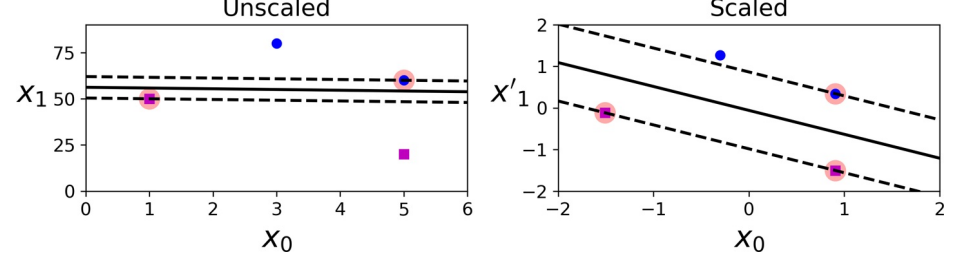
\includegraphics[scale=0.9]{figures/svm_scale.png}
	\caption{ Чувствительность к масштабам признаков. SVM посчитал горизонтальное положение полосы наиболее удачным, так как по оси $ x_1 $ масштаб больше и соответственно получается большее значении ширины зазаора }\label{fig:svm_scale}
\end{figure}

\emph{Классификация с жестким зазором} (hard margin classification) присущи две главные проблемы. Во-первых, она работает, только если данные \emph{линейно-сепарабельны}. Во-вторых, она довольно чувствительна к выбросам.

Чтобы избежать этих проблем, предпочтительнее применять более гибкую модель. Цель заключается в том, чтобы отыскать хороший баланс между удержанием полосы как можно более широкой и ограничением количества нарушений зазора. Это называется \emph{классификацией с мягким зазором} (soft margin classification)

В классах SVM библиотеки Scikit-Learn управлять упомянутым балансом можно с помощью параметра $ C $: меньшее значение $ C $ ведет к более широкой полосе, но большему числу нарушений зазора.

\verb|LinearSVC(C=1, loss="hinge")| похож на \verb|SVC(kernel="linear", C=1)| с точки зрения фунциональных возможностей, но основан на библиотеке liblinear\footnote{Библиотека liblinear реализует специальный алгоритм для \underline{\itshape линейных} методов SVM -- метод двойного покоординатного спуска (dual coordinate descent) \url{https://www.csie.ntu.edu.tw/~cjlin/papers/cddual.pdf}}, а не libsvm, работает гораздо быстрее и лучше масштабируется на большие выборки \cite[\strbook{202}]{geron:hands_on_ml}. Для улучшения производительности следует установить гиперпараметр \verb|dual| в \verb|False|. Флаг \verb|dual=True| означает, что будет решаться \emph{двойственная задача} (dual problem), а не \emph{прямая задача} (primal problem).

Рекомендуется (см.~\href{https://scikit-learn.org/stable/modules/generated/sklearn.svm.LinearSVC.html}{LinearSVC}) оптимизационную задачу решать в \emph{прямой} постановке (т.е. \verb|dual=False|), когда в матрице признакового описания объекта экезмпляров больше, чем признаков -- $ \text{n\_samples} > \text{n\_features} $ (книжная ориентация матрицы).

То есть оптимизационная задача для классификатора \verb|LinearSVC| может быть сформулирована как в \emph{прямой}, так и в \emph{двойственной} постановке.

\remark{
Ядерный трюк предотвращает комбинаторно бурный рост количества признаков, поскольку в действительности мы не добавляем никаких признаков
}

Класс \verb|LinearSVC| основан на библиотеке liblinear, не поддерживает ядерный трюк, но масштабируется почти линейно с ростом числа экземпляров $ m $ и числа признаков $ n $, а его временная сложность составляет $ \approx O(m \times n) $.

Класс \verb|SVC| основан на библиотеке libsvm и поддерживает ядерный трюк. Временная сложность обычно находится между $ O(m^2 \times n) $ и $ O(m^3 \times n) $. Это означает, что он становится невероятно медленным при большом количестве обучающих экземпляров (порядка нескольких сотен тысяч). Такой алгортим идеален для сложных, но небольших или средних обучающих наборов. Тем не менее, он хорошо масштабируется с ростом числа признаков, особенно разреженных.

Метод опорных векторов поддерживает не только \emph{линейную} и \emph{нелинейную} \underline{классификацию}, но и \emph{линейную} и \emph{нелинейную} \underline{регрессию}.

Регрессия SVM пытается уместить \emph{на полосе} как можно больше экземпляров наряду с ограничением нарушений зазора (т.е. экземпляров вне полосы) \cite[\strbook{210}]{geron:hands_on_ml}. Ширина полосы управляется гиперпараметром $ \varepsilon $ (\pic{fig:svm_linreg}).

\begin{figure}[h]
	\centering
	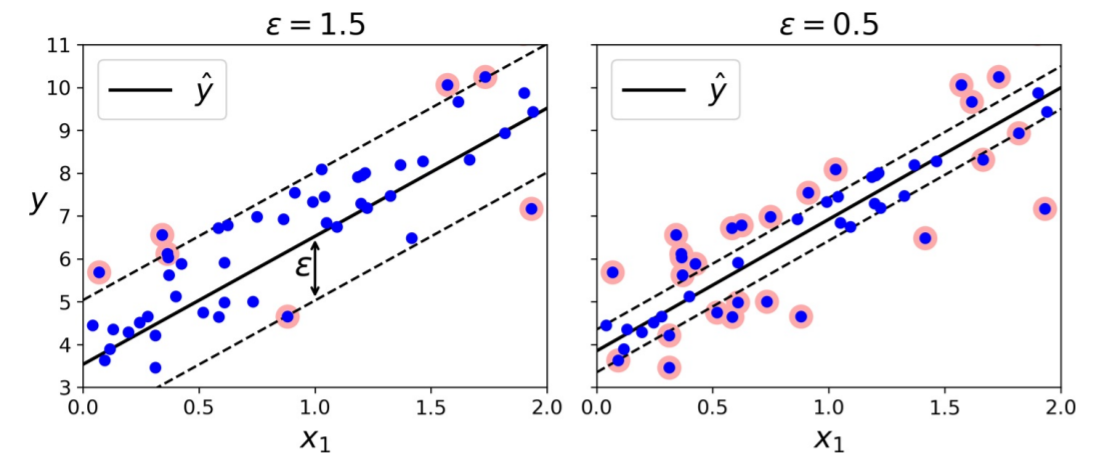
\includegraphics[scale=0.7]{figures/svm_linreg.png}
	\caption{ Линейная регрессия с помощью LinearSVR }\label{fig:svm_linreg}
\end{figure}

Добавление дополнительных обучающих экземпляров внутри зазора не влияет на прогнозы модели; потому говорят, что модель \emph{нечувствительна} к $ \varepsilon $.

Для решения задач \emph{линейной} регрессии можно использовать класс \verb|LinearSVR|, а для задач \emph{нелинейной} регрессии -- \verb|SVR|.

\begin{figure}[h]
	\centering
	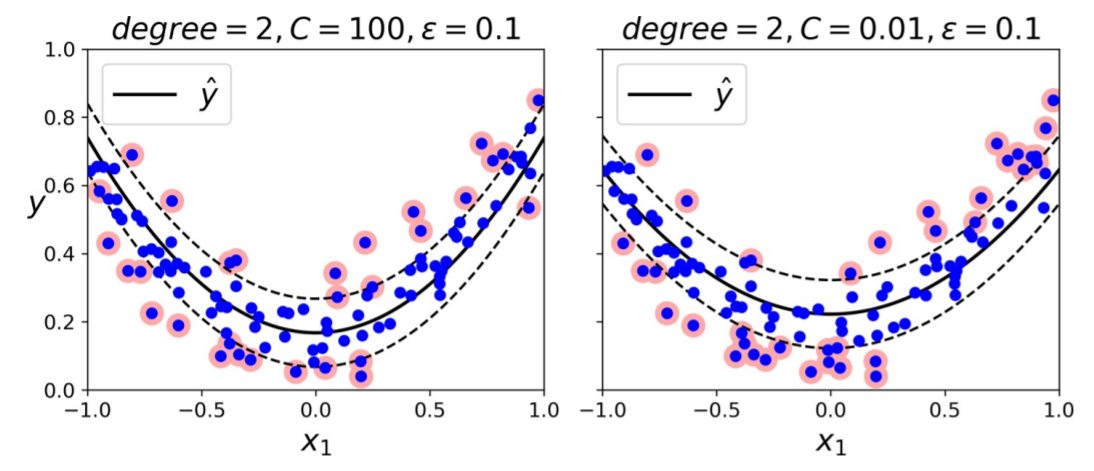
\includegraphics[scale=0.7]{figures/svm_nonlinreg.png}
	\caption{ Нелинейная регрессия с помощью SVR с полиномиальным ядром 2-ого порядка }\label{fig:svm_nonlinreg}
\end{figure}

\remark{
Класс SVR, как и SVC поддерживает ядерный трюк
}

Если в задаче $ n $ признаков, то \emph{функция решения}\footnote{decision function} -- это $ n $-мерная гиперплоскость (\pic{fig:svm_des_fun}), а \emph{граница решения}\footnote{decision boundary} (то есть множество точек, где функция решения равна нулю) -- это $ (n - 1) $-мерная гиперплоскость \cite[\strbook{212}]{geron:hands_on_ml}.

\begin{figure}[h]
	\centering
	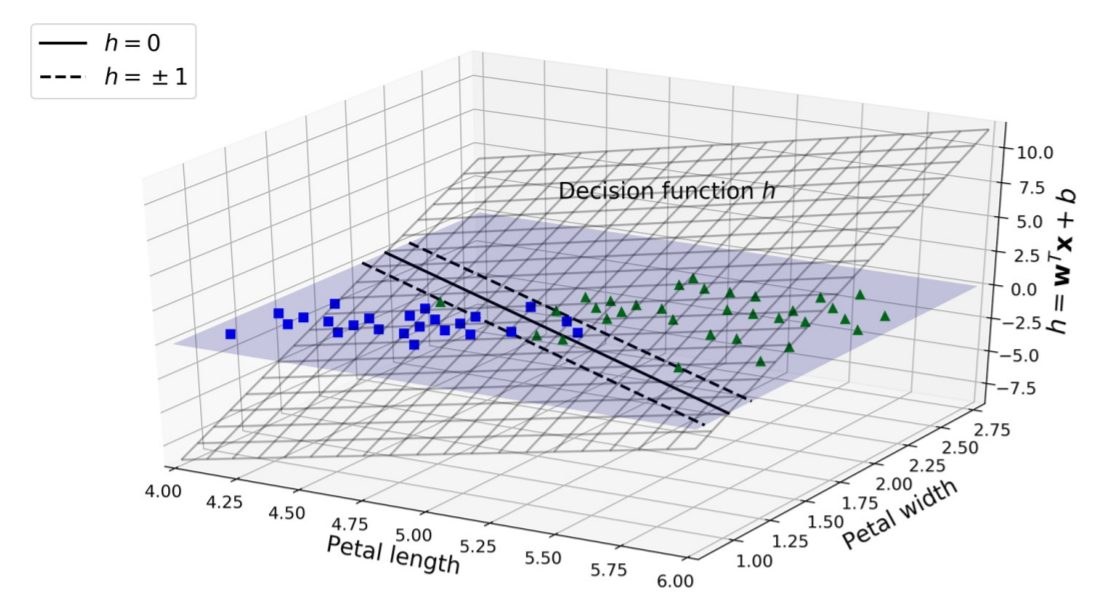
\includegraphics[scale=0.7]{figures/svm_des_fun.png}
	\caption{ Функция решения для набора данных об ирисах }\label{fig:svm_des_fun}
\end{figure}

Обучение линейного классификатора SVM означает нахождение таких значений $ \{w_1, \ldots, w_n\}, b $, которые делают \emph{зазор} как можно более \emph{широким}, одновременно \emph{избегая} нарушений зазора (жесткий зазор) или \emph{ограничивая} их (мягкий зазор) \cite[\strbook{213}]{geron:hands_on_ml}.

Задачи \emph{жесткого} и \emph{мягкого зазора} являются задачами выпуклой \emph{квадратичной} оптимизации с \emph{линейными} ограничениями \cite[\strbook{215}]{geron:hands_on_ml}. Такие задачи известны как задачи квадратичного программирования (Quadratic Programming -- QP).

То есть перейдя от оригинальной задачи (\emph{прямая задача}) с помощью метода множителей Лагранжа и записав условия Каруша-Куна-Таккера, приходим к \emph{двойственной задаче} и решаем ее (находим множители Лагранжа) методами квадратичного программирования.

Двойственная задача решается быстрее прямой, когда количество обучающих экземпляров меньше количества признаков. Но что более важно, в случае двойственной задачи становится возможен ядерный трюк, в то время как при решении прямой задачи он невозможен.

Ядро -- это функция, которая способна вычислять скалярное произведение $ \varphi(\mathbf{a})^T \cdot \varphi (\mathbf{b}) $, базируясь только на исходных векторах $ \mathbf{a} $ и $ \mathbf{b} $, без необходимости вычислять трансформацию $ \varphi $ (или даже знать о ней) \cite[\strbook{218}]{geron:hands_on_ml}.

\subsubsection{Из курса лекций Соколова}

Вспомним, что метод опорных векторов сводится к решению задачи оптимизации (для общего случая \emph{классификации} с мягким зазором с помощью SVC)
\begin{align*}
	\begin{cases}
		\dfrac{1}{2} \| w \|^2 + C \sum\limits_{i=1}^{l} \xi_i \to \min\limits_{ w, b, \xi }\\
		y_i ( \langle w, x_i \rangle + b) \geqslant 1 - \xi_i, \ i = 1, \ldots, l,\\
		\xi_i \geqslant 0, \ i = 1, \ldots, l.
	\end{cases}
\end{align*}

Построим \emph{двойственную} к ней. Запишем \emph{лагранжиан} (ограничения\footnote{Ограничения должны быть сведены к виду $ left\_part \geqslant 0 $} просто суммируются с учетом множителей Лагранжа $ \lambda_i, \mu_i $ и вычитаются из целевой функции)
\begin{align*}
	L(w, b, \xi, \lambda, \mu) = \dfrac{1}{2} \| w \|^2 + C \sum_{i=1}^{l} \xi_i - \sum_{i=1}^{l} \lambda_i [\, y_i (\langle w, x_i \rangle + b) - 1 + \xi_i \,] - \sum_{i=1}^{l} \mu_i \xi_i.
\end{align*}

Выпишем условия Каруша-Куна-Таккера
\begin{align}
	\nabla_w L = w - \sum_{i=1}^{l} \lambda_i y_i x_i = 0 \qquad &\Rightarrow w = \sum_{i=1}^{l} \lambda_i y_i x_i \label{eq:w}\\
	\nabla_b L = - \sum_{i=1}^l \lambda_i y_i = 0 \qquad &\Rightarrow \sum_{i=1}^l \lambda_i y_i = 0 \\
	\nabla_{\xi_i} L = C - \lambda_i - \mu_i \qquad &\Rightarrow \lambda_i + \mu_i = C \\
	\lambda_i [\, y_i ( \langle w, x_i \rangle + b) - 1 + \xi_i \,] = 0 \qquad &\Rightarrow (\lambda_i = 0) \ \text{или} \ (y_i ( \langle w, x_i \rangle + b ) = 1 - \xi_i) \label{eq:xi} \\
	\mu_i \xi_i = 0 \qquad &\Rightarrow (\mu_i = 0) \  \text{или} \ (\xi_i = 0) \\
	\xi_i \geqslant 0, \lambda_i \geqslant 0, \mu_i \geqslant 0.
\end{align}

При вычислении градиентов $ \nabla_w, \nabla_b, \nabla_{\xi_i} $ просто берем частные производные от лагранжиана $ L $ по каждому элементу $ w_1, w_2, \ldots $ вектора $ w $, по каждому элементу $ b_1, b_2, \ldots $ вектора $ b $ и т.д.

Проанализируем полученные условия. Из \eqref{eq:w} следует, что вектор весов $ w $, полученный в результате настройки SVM, можно записать как линейную комбинацию объектов $ x_i $ из объектов обучающей выборки, причем веса в этой линейной комбинации можно найти как решение двойственной задачи.

В зависимости от значений $ \xi_i $ и $ \lambda_i $ объекты $ x_i $ разбиваются на три категории:
\begin{enumerate}
	\item $ \xi_i = 0, \lambda_i = 0 $: такие объекты не влияют на решение $ w $ (входят в него с нулевым весом $ \lambda_i $), правильно классифицируются ($ \xi_i = 0 $) и лежат вне разделяющей полосы. Объекты этой категории называются \emph{периферийными}.
	
	\item $ \xi_i = 0, 0 < \lambda_i < C $: из условия \eqref{eq:xi} следует, что $ y_i ( \langle w, x_i \rangle + b ) = 1 $, то есть объект лежит \emph{строго на границе разделяющей полосы}. Поскольку $ \lambda_i > 0 $, объект влияет на решение $ w $. Объекты этой категории называются \emph{опорными граничными}.
	
	\item $ \xi_i > 0, \lambda_i = C $: такие объекты могут лежать внутри разделяющей полосы ($ 0 < \xi_i < 2 $) или выходить за ее пределы ($ \xi_i \geqslant 2 $). При этом если $ 0 < \xi_i < 1 $, то объект классифицируется правильно, в противном случае неправильно. Объекты этой категории называются \emph{опорными нарушителями}.
\end{enumerate}

Итак, итоговый классификатор зависит от объектов, лежащих на границе разделяющей полосы, и от объектов-нарушителей (c $ \xi_i > 0 $).

Приходим к следующей \emph{двойственной задаче}
\begin{align*}
	\begin{cases}
	    \sum\limits_{i=1}^{l} \lambda_i - \dfrac{1}{2} \sum\limits_{i,j=1}^{l} \lambda_i \lambda_j y_i y_j \langle x_i, x_j \rangle \to \max\limits_\lambda \\
	    0 \leqslant \lambda_i \leqslant C, \ i = 1, \ldots, l, \\
	    \sum\limits_{i=1}^{l} \lambda_i y_i = 0.
	\end{cases}
\end{align*}

\noindent Она также является вогнутой, квадратичной и имеет единственный максимум.

Двойственная задача SVM зависит только от скалярных произведений объектов -- отдельные признаковые описания никак в нее не входят. Значит, можно легко сделать ядровый переход
\begin{align*}
	\begin{cases}
		\sum\limits_{i=1}^l \lambda_i - \dfrac{1}{2} \sum\limits_{i,j=1}^l \lambda_i \lambda_j y_i y_j K(x_i, x_j) \to \max\limits_\lambda \\
		0 \leqslant \lambda_i \leqslant C, \ i = 1, \ldots, l, \\
		\sum\limits_{i=1}^l \lambda_i y_i = 0.
	\end{cases}
\end{align*}

Подставляя представление \eqref{eq:w} в классификатор, получаем
\begin{align*}
	a({\color{blue}x}) = \text{sign} \Big( \sum_{i=1}^l \lambda_i y_i \langle x_i, {\color{blue}x} \rangle + b \Big).
\end{align*}

Таким образом, {\color{blue}классификатор измеряет \emph{сходство} \underline{нового объекта} с \underline{объектами из обучающей выборки}, вычисляя \emph{скалярное произведение} между ними}. Это выражение также зависит только от скалярных произведений, поэтому в нем тоже можно сделать переход к ядру.

Если использовть гауссовское ядро (радиальную базисную функцию) в \emph{методе опорных векторов}, то получится следующее \emph{решающее правило}
\begin{align*}
	a({\color{blue}x}) = \text{sign} \sum_{i=1}^l y_i \lambda_i \underbrace{\exp \Bigg( - \dfrac{ \| {\color{blue}x} - x_i \|^2 }{ 2 \sigma^2 } \Bigg)}_{K(x, x_i)}
\end{align*}

То есть мы просто в решающем правиле заменили \emph{скалярное произведение} $ \langle x_i, x \rangle $ на \emph{ядро} $ K(x, x_i) $.

\subsubsection{Из книги Буркова}

После обучения алгоритм метода опорных векторов будет определяться так
\begin{align*}
	f(\mathbf{x}) = \text{sign} (\mathbf{w}^* \mathbf{x} - b^*)
\end{align*}

Чтобы с помощью модели метода опорных векторов предсказать, является ли электронное письмо спамом или нет, нужно взять текст письма, преобразовать его в вектор признаков, затем умножить этот вектор на $ \mathbf{w}^{*} $, вычесть $ b^{*} $ и взять знак результата. Это даст прогноз (+1 означает <<спам>>, а -1 означает <<не спам>>).

Но как машина находит $ \mathbf{w}^{*} $ и $ b^{*} $? Она решает задачу оптимизации. Машины хорошо справляются с оптимизацией функций в условиях ограничений.

Итак, какие ограничения должны удовлетворяться здесь? Прежде всего, модель должна правильно предсказывать метки имеющихся 10 000 данных. Каждый образец задается парой $ (\mathbf{x}_i, y_i) $, где $ \mathbf{x}_i $ -- вектор признаков $ i $-го образца, а $ y_i $ -- его метка, которая принимает значение -1 или +1. Ограничения выглядят следующим образом \cite{burkov:2020} 
\begin{align*}
	\mathbf{w} \mathbf{x}_i + b\geqslant +1, \text{если} \ y_i = +1,\\
	\mathbf{w} \mathbf{x}_i + b\leqslant -1, \text{если} \ y_i = -1.
\end{align*}

Желательно также, чтобы гиперплоскость отделяла положительные данные от отрицательных с максимальным зазором. Зазор -- это расстояние между ближайшими образцами двух классов ,отделяемых границей принятия решения.

Большой зазор способствует  лучшему обобщению, то есть тому, насколько хорошо модель будет классифицировать новые данные.

Для \emph{максимизации зазора} нужно \emph{минимизировать эвклидову норму} $ \| \mathbf{w} \| = \sqrt{ \sum\limits_{j=1}^D (w^{(j)})^2 }$ \cite[\strbook{23}]{burkov:2020}, так как расстояние между границами определяется как $ \dfrac{2}{ \| \mathbf{w} \| } $.

{В методе опорных векторов решается следующая задача \emph{оптимизации}: минимизировать эвклидову норму  $ \| \mathbf{w} \| $ с учетом $ y_i (\mathbf{w} \mathbf{x}_i - b) \geqslant 1, \ i = 1, \ldots, N $}

Рассмотренная версия алгоритма строит \emph{линейную модель} (граница принятия решения -- это прямая линия, плоскость или гиперплоскость). Однако метод опорных векторов также может включать \emph{ядра}, способные сделать границу решения \emph{произвольно нелинейной}.

\remark{
\emph{Градиент} -- обобщение понятия производной на случай скалярной функции векторного аргумента. Другими словами градиент -- вектор частных производных
}

В некотрых случаях невозможно полностью разделить две группы точек из-за шума в данных, ошибок разметки или аномалий (данных, сильно отличающихся от <<типичного>> образца в наборе данных). Для таких случаев есть версия алгоритма SVM, способная включить гиперпараметр штрафа за неправильную классификацию обучающих данных конкретных классов.

\remark{
Для того чтобы понять связь между ошибкой модели, размером обучающего набора, формой математического уравнения, определяющего модель, и временем построения модели, следует прочитать о \emph{вероятностно-приблизительное корректном обучении} (Probably Approximately Correct, PAC). Теория вероятностно-приблизительного корректного обучения поможет проанализировать и понять, сможет ли и при каких условиях алгоритм обучения получить приблизительно корректный классификатор 
}

Минимизация $ \| w \| $ эквивалентна минимизации $ \dfrac{1}{2} \| w \|^2 $. Тогда оптимизационную задачу для метода опорных векторов можно переписать так (алгоритм метода опорных векторов с \underline{жестким зазором}\footnote{hard-margin SVM})
\begin{align}\label{eq:svm_hard_margin}
	\min \dfrac{1}{2} \| w \|^2,\ \text{такое, что}\ y_i (\mathbf{x}_i \mathbf{w} - b) - 1\geqslant 0, \ i = 1,\ldots, N.
\end{align}

Чтобы распространить SVM на случаи, когда данные невозможно разделить линейно, введем \emph{кусочно-линейную функцию потерь} (hinge loss function): $ \max (0; 1 - y_i (\mathbf{w} \mathbf{x}_i - b)) $.

Кусочно-линейная функция потерь равна нулю, если прогноз $ \mathbf{w} \mathbf{x}_i $ лежит с правильной стороны от границы решения, так как в этом случае правая часть кусочно-линейной функции потерь будет отрицательна. Для данных, лежащих с неправильной стороны, значение функции пропорционально расстоянию от границ решения.

Алгоритм метода опорных векторов, оптимизирующий кусочно-линейную функцию потерь, называют методом опорных векторов с \underline{мягким зазором} (soft-margin SVM)
\begin{align*}
	\| \mathbf{w} \|^2 + C \dfrac{1}{N} \sum_{i=1}^N \max \big(0; 1 - y_i (\mathbf{w} \mathbf{x}_i - b)\big),
\end{align*}
где $ C $ -- гиперпараметр, определяющий компромисс между увеличением размера границы решения и гарантией местонахождения каждого $ \mathbf{x}_i $ с правильной стороны от границы решения.

SVM можно адаптировать для работы с наборами данных, которые нельзя разделять гиперплоскостью в исходном пространстве. Действительно, если удастся преобразовать исходное пространство в пространство более высокой размерности, можно надеяться, что данные станут линейно сепарабельны в этом преобразованом пространстве.

Использование функции для \underline{неявного} преобразования исходного пространства в пространство более высокой размерности в ходе оптимизации функции стоимости в SVM называется \emph{ядерным трюком} (kernel trick).

Чтобы понять, как работают ядра, прежде нужно посмотреть, как алгоритм оптимизации для SVM находит оптимальные значения для $ \mathbf{w} $ и $ b $.

Для решения задачи оптимизации \eqref{eq:svm_hard_margin} традиционно используется \emph{метод множителей Лагранжа}. Вместо оригинальной задачи проще решить эквивалентную задачу, сформулированную так
\begin{align*}
	\max_{ \alpha_1, \ldots, \alpha_N } \sum_{i=1}^N \alpha_i - \dfrac{1}{2} \sum_{i=1}^{N} \sum_{i=1}^N y_i \alpha_i (\mathbf{x}_i \mathbf{x}_k) y_k \alpha_k\ \text{при условии, что} \ \sum_{i=1}^N \alpha_i y_i = 0\ \text{и} \ \alpha_i \geqslant 0, i = 1, \ldots, N,
\end{align*}
где $ \alpha_i $ называются множителями Лагранжа.

В такой формулировке задача оптимизации превращается в выпуклую задачу квадратичной оптимизации, которая эффективно решается применением алгоритмов квадратичного программирования.

Чтобы преобразовать \emph{исходное векторное пространство} в \emph{пространство с большим числом измерений}, нужно преобразовать $ \mathbf{x}_i $ в $ \varphi( \mathbf{x}_i ) $ и $ \mathbf{x}_k $ в $ \varphi( \mathbf{x}_k ) $, а затем перемножить $ \varphi( \mathbf{x}_i ) $ и $ \varphi( \mathbf{x}_k ) $. Эти вычисления могут оказаться очень дорогостоящими.

С другой стороны, нас интересует только результат скалярного произведения $ \mathbf{x}_i \mathbf{x}_k $, который, как мы знаем, является действительным числом. Нам все равно, как будет получено это число, лишь бы оно было верным. Используя функцию ядра, можно избавиться от дорогостоящего преобразования исходных векторов признаков в векторы с более высокой размерностью и избежать необходимости вычислять их скалярное произведение. Мы заменим эти вычисления простой операцией с исходными векторами признаков, которая даст тот же результат.

Например, вместо преобразования $ (q_1, p_1) \to (q_1^2, \sqrt{2} q_1 p_1, ;p_1^2) $ и $ (q_1, p_2) \to (q_2^2, \sqrt{2} q_2 p_2, p_2^2) $ и последующего вычисления скалярного произведения $ (q_1^2, \sqrt{2} q_1 p_1, p_1^2) $ и $ (q_2^2, \sqrt{2} q_2 p_2, p_2^2) $, чтобы получить $ (q_1^2 q_2^2 + 2 q_1 q_2 p_1 p_2 + p_1^2 p_2^2) $, можно найти скалярное прозведение $ (q_1, p_1) $ и $ (q_2, p_2) $, чтобы получить $ (q_1 q_2 + p_1 p_2) $, а затем возвести в квадрат, чтобы получить тот же результат $ (q_1^2 q_2^2 + 2 q_1 q_2 p_1 p_2 + p_1^2 p_2^2) $.

Это был пример функции ядра, и мы использовали квадратичное ядро $ k( \mathbf{x}_i \mathbf{x}_k )  \mathrel{ \stackrel{\rm def}{=} ( \mathbf{x}_i \mathbf{x}_k )^2 } $.

Существует несколько функций ядра, из которых наиболее широко используется \emph{радиальная базисная функция} (гауссово ядро, RBF)
\begin{align*}
	k( \mathbf{x}, \mathbf{x}^{'} ) = \exp \Big( - \dfrac{ \| \mathbf{x} - \mathbf{x}^{'} \|^2 }{ 2 \sigma^2 } \Big),
\end{align*}
где $ \| \mathbf{x} - \mathbf{x}^{'} \|^2 $ -- квадрат евклидова расстояния между двумя векторами признаков.

Евклидово расстояние определяется следующим уравнением
\begin{align*}
	d( \mathbf{x}_i, \mathbf{x}_k ) \mathrel{ \stackrel{\rm def}{=} } \sqrt{ \sum_{j=1}^D \big( x_i^{(j)} - x_k^{(j)} \big)^2 }.
\end{align*}

\subsection{Метод k ближайших соседей}

Метод k ближайших соседей -- это непараметрический алгоритм обучения. В отличие от други алгоритмов обучения, позволяющих отбрасывать обучающие данные после построения модели, метод kNN сохраняет все обучающие экземпляры в памяти. Когда появится новый, ранее не встречавшийся образец, алгоритм kNN находит $ k $ обучающих данных, наиболее близких к $ \mathbf{x} $, и возвращает наиболее часто встречающуюся метку в случае классификации или среднее значение метки в случае регрессии.

Близость двух экземпляров данных определяется функцией расстояния. Нередко используется \emph{косинусное сходство}
\begin{align*}
	s( \mathbf{x}_i, \mathbf{x}_k ) \mathrel{ \stackrel{\rm def}{=} } \dfrac{ \sum\limits_{j=1}^D x_i^{(j)} x_k^{(j)} }{ \sqrt{ \sum\limits_{j=1}^D \big( x_i^{(j)} \big)^2 } \sqrt{ \sum\limits_{j=1}^D \big( x_k^{(j)} \big)^2 } },
\end{align*}
которая является мерой сходства двух векторов.

\subsection{Многослойный персептрон}

Нейронная сеть, так же как модель регрессии или SVM, -- это всего лишь математическая функция $ y = f_{NN}(\mathbf{x}) $. Функция $ f_{NN} $ имеет особую форму: это вложенная функция (вроде матрешки). Например, для трехслойной нейронной сети, возвращающей скаляр, $ f_{NN} $ выглядит так \cite[\strbook{91}]{burkov:2020}
\begin{align*}
	y = f_{NN}(\mathbf{x}) = f_3(\mathbf{f}_2(\mathbf{f}_1(\mathbf{x}))),
\end{align*}
где $ \mathbf{f}_1 $ и $ \mathbf{f}_2 $ в уравнении выше -- это векторные функции, которые определяются как
\begin{align*}
	\mathbf{f}_l (\mathbf{z}) \mathrel{\stackrel{\rm def }=} \mathbf{g}_l (\mathbf{W}_l \mathbf{z} + \mathbf{b}_l),
\end{align*}
где $ l $ -- это индекс слоя и может охватывать от 1 до любого количества слоев; $ \mathbf{g}_l $ -- функция активации.

Параметры $ \mathbf{W}_l $ (матрица) и $ \mathbf{b}_l $ (вектор) определяются для каждого слоя в ходе обучения, с использованием градиентного спуска для оптимизации.

Важный момент: здесь вместо вектора $ \mathbf{w}_l $ используется матрица $ \mathbf{W}_l $. Причина в том, что $ \mathbf{g}_l $ -- векторная функция. Каждая строка $ \mathbf{w}_{l, u} $ ($ u $ означает <<узел>>) в матрице $ \mathbf{W}_l $ является вектором той же размерности, что и $ \mathbf{z} $.

Пусть $ a_{l, u} = \mathbf{w}_{l, u} \mathbf{z} + b_{l, u} $. На выходе $ \mathbf{f}_l(\mathbf(z)) $ возвращает вектор $ \{ g_l(a_{l,1}), g(a_{l,2}), \ldots, g_l(a_{l, size_l}) \} $, где $ g_l $ -- некоторая скалярная функция (возвращает скаляр, а не вектор), $ size_l $ -- количество узлов в $ l $-ом слое.

\begin{figure}[h]
	\centering
	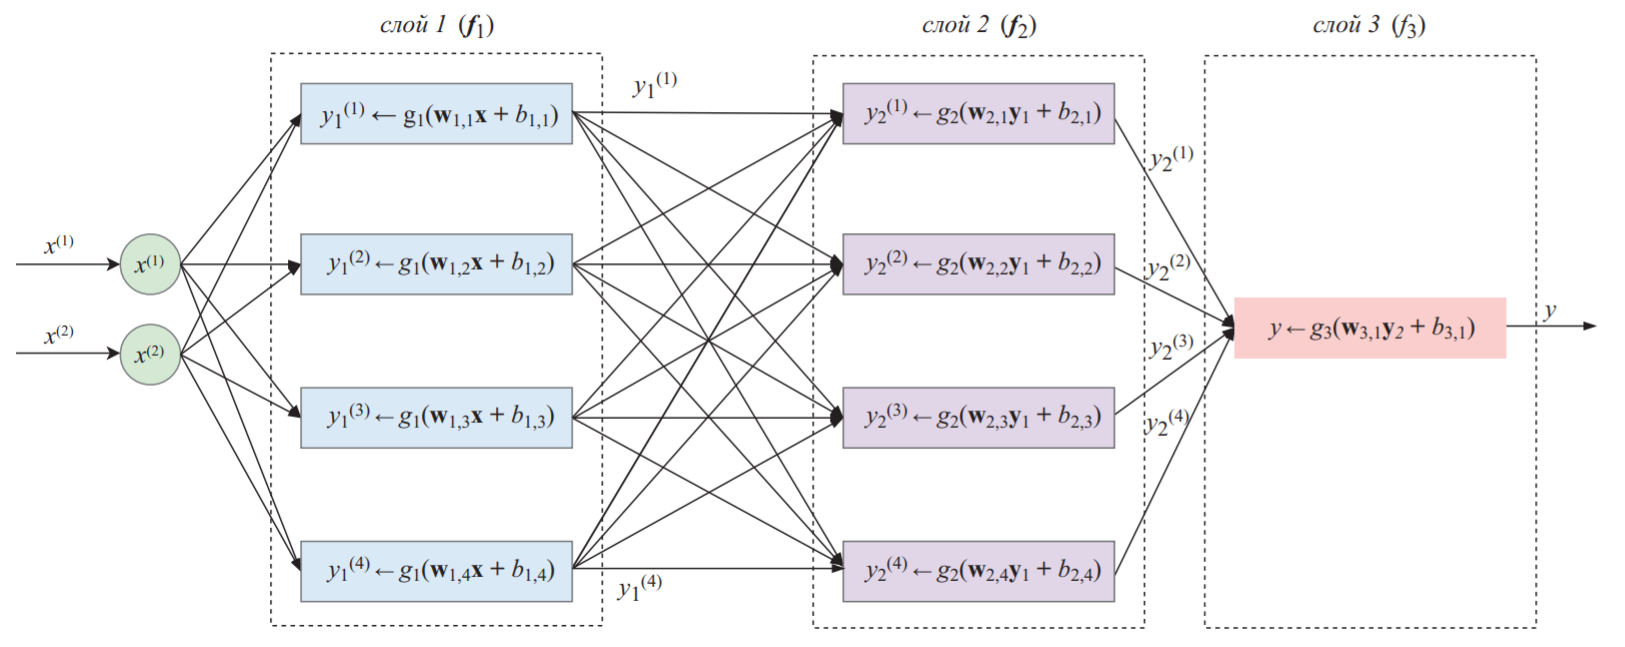
\includegraphics[scale=0.6]{figures/MLP.png}
	\caption{ Многослойный персептрон с двумерным входом, двумя слоями по четыре узла в каждом и выходным слоем с единственным узлом }\label{fig:MLP}
\end{figure}

Основная цель \emph{нелинейных} компонентов в функции $ f_{NN} $ состоит в том, чтобы позволить нейронной сети аппроксимировать \emph{нелинейные функции}. В отсутствие нелинейных компонентов $ f_{NN} $ была бы линейной, независимо от количества слоев. Причина в том, что $ \mathbf{W}_l z + \mathbf{b} $ является \underline{линейной} функцией, а линейная функция от линейной функции также является \underline{линейной}.

\section{Глубокое обучение}

Под глубоким обучением подразумевается обучение нейронных сетей, имеющих больше двух невыходных слоев. В прошлом обучение таких сетей усложнялось все больше с ростом количества слоев. В числе самых больших проблем назывались \emph{взрывной рост градиента} и \emph{затухание градиента}, поскольку для определения параметров сети использовался градиентный спуск.

Если проблема взрывного роста градиента решалась относительно просто, с применением таких простых методов, как \emph{ограничение градиента} и \emph{L1- или L2-регуляризация}, то проблема затухания градиента оставалась неразрешимой в течение десятилетий.

Для обновления значений параметров в нейронных сетях обычно используется алгоритм \emph{обратного распространения}. Обратное распространение -- это эффективный алгоритм вычисления \underline{градиентов} в нейронных сетях с использованием правила дифференцирования сложных функций.

\remark{
В каждой итерации обучения, в процессе градиентного спуска, параметры нейронной сети обновляются \underline{пропорционально} частной производной функции потерь для текущего параметра
}

Проблема в том, что иногда \emph{градиент} оказывается \emph{исчезающе малым}, что фактически мешает изменению значений некоторых параметров. В худшем случае это может \emph{полностью остановить обучение} нейронной сети.

Традиционные функции активации, такие функция гиперболического тангенса имеют градиенты в диапазоне $ (0, 1) $, при этом градиенты вычисляются на этапе обратного распространения по правилу дифференцирования сложных функций. В результате для вычисления градиентов предыдущих слоев (расположенных \emph{левее}) в $ n $-слойной сети производится перемножение $ n $ этих небольших чисел, из-за чего градиент экспоненциально уменьшается с увеличением $ n $. Это приводит к тому, что \emph{более ранние слои} обучаются намного \emph{медленее}, если вообще обучаются \cite[\strbook{96}]{burkov:2020}.

Однако современные реализации алгоритмов обучения нейронных сетей позволяют эффективно обучать очень глубокие нейронные сети (до нескольких сотен слоев). Это объясняется внедрением целого комплекса усовершенствований, включая ReLU, LSTM (и другие вентильные узлы), а также таких методов, как соединение с пропуском слоя, используемые в остаточных нейронных сетях, а также усовершенствованные версии алгоритма градиентного спуска.

\remark{
Когда в роли обучающих данных используются изображения, входные данные получаются слишком многомерными. Так как каждый пиксель в изображении -- это отдельный признак
}

\subsection{Сверточная нейронная сеть}

\emph{Сверточная нейронная сеть} (CNN) -- это особый вид сетей прямого распространения, который значительно сокращает количество параметров в глубокой нейронной сети с большим количеством узлов практически без потери качества модели.

Учитывая, что наиболее важная информация занимает на изображении ограниченную площадь, мы можем разделить изображение на квадратные фрагменты, используя метод скользящего окна. Затем обучить несколько \emph{небольших регрессионных моделей} одновременно, передавая каждой квадратный фрагмент.

Цель каждой небольшой регрессионной модели -- научиться обнаруживать определенный шаблон во фрагменте на вход. Например, одна небольшая модель может научиться определять небо, другая -- траву, третья -- края зданий и т.д.

Небольшие регрессионные модели в CNN напоминают модель многослойного персептрона, но имеют \emph{только по одному слою} \cite[\strbook{98}]{burkov:2020}. Чтобы обнаружить какой-либо шаблон, модель регрессии должна \emph{определить параметры матрицы} $ \mathbf{F}_{p \times p} $. Некотрый фрагмент может выглядеть как следующая матрица $ \mathbf{P} $
\begin{align*}
	\mathbf{P} =
	\begin{pmatrix}
		0 & 1 & 0 \\
		1 & 1 & 1 \\
		0 & 1 & 1
	\end{pmatrix}
\end{align*}

Этот фрагмент представляет шаблон с изображением креста. Небольшая регрессионная модель, которая будет обнаруживать такие шаблоны (и только их), должна обучить матрицу $ \mathbf{F} $ размером $ 3 \times 3 $, в которой параметры в позициях, соответствующих единицам во входном фрагменте, будут положительными цислами, а параметры в позициях, соотвествующих нулям, будут иметь значения, близкие к нулю. Если вычислить свертку матриц $ \mathbf{P} $ и $ \mathbf{F} $, полученное значение будет тем больше, чем больше $ \mathbf{F} $ похожа на $ \mathbf{P} $.

Оператор свертки определен только для матриц, имеющих одинаковое количество строк и столбцов (\pic{fig:conv}).

\begin{figure}[h]
	\centering
	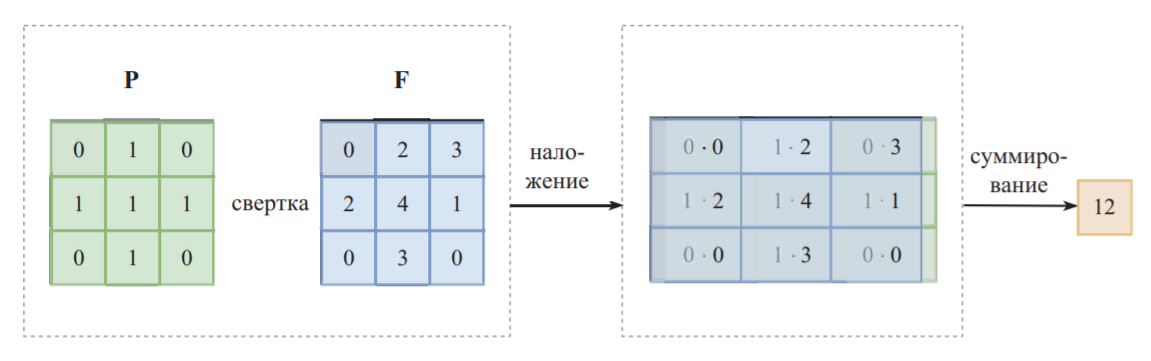
\includegraphics[scale=0.6]{figures/conv.png}
	\caption{ Свертка двух матриц }\label{fig:conv}
\end{figure}

Например, если подать на вход фрагмент $ \mathbf{P} $, имеющий L-шаблон
\begin{align*}
	\mathbf{P} = 
	\begin{pmatrix}
		1 & 0 & 0 \\
		1 & 0 & 0 \\
		1 & 1 & 1
	\end{pmatrix},
\end{align*}
тогда свертка с $ \mathbf{F} $ даст в результате меньшее значение: 5.

\remark{
То есть чем больше фрагмент похож на фильтр, тем выше значение операции свертки
}

Каждый фильтр в первом (самом левом) слое скользит -- свертывает -- по входному изображению слева направо, сверху вниз, и в каждой итерации вычисляет значение свертки.

\underline{Матрица фильтра} (по одной для каждого фильтра в каждом слое) и \underline{значения смещения} являются \emph{обучаемыми параметрами}, которые оптимизируются с испльзованием градиентного спуска с обратным распространением.

Нелинейность применяется к сумме свертки и смещения, т.е. $ \sigma (\mathbf{P} \circ \mathbf{F} + b) $. Как правило, во всех скрытых слоях используется функция активации ReLU. Функция активации в выходном слое зависит от решаемой задачи. Функция активации в выходном слое зависит от решаемой задачи.

Если CNN имеет один сверточный слой, следующий за другим сверточным слоем, то последующий слой $ l + 1 $ будет обрабатывать выходные данные предыдущего слоя $ l $, как коллекцию $ size_l $ матриц изображения. Такая коллекция называется \emph{томом}. Размер колллекции называется \emph{глубиной тома}. Каждый фильтр в слое $ l + 1 $ выполняет свертку \underline{всего тома}. Свертка фрагмента тома -- это просто сумма сверток соответствующих фрагментов отдельных матриц, из которых состоит том.

\begin{figure}[h]
	\centering
	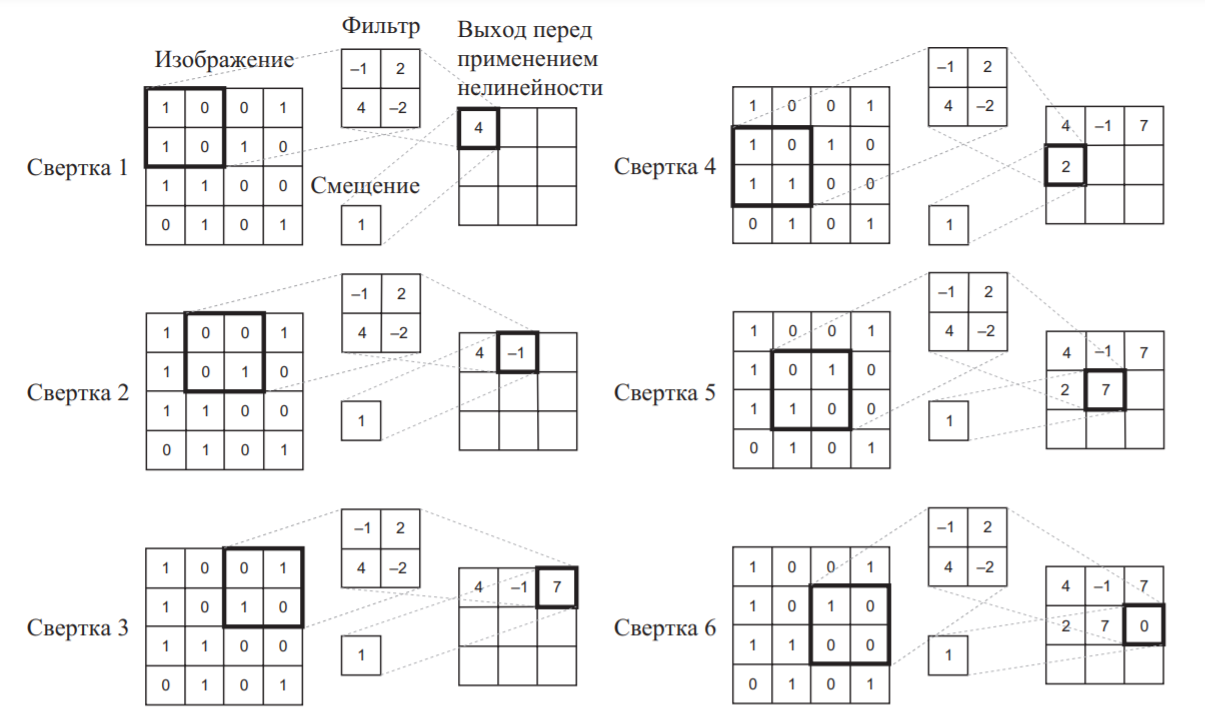
\includegraphics[scale=0.7]{figures/conv-3.png}
	\caption{ Фильтр, свертывающий изображение }\label{fig:conv-3}
\end{figure}

Свертки имеют два важных свойства -- шаг и дополнение. Шаг -- это величина одного шага смещения окна. Дополнение позволяет получить увеличенную выходную матрицу. Это ширина рамки с дополнительными ячейками, которые добавляются вокруг изображения (или тома) перед сверткой с помощью фильтра. Обычно дополнительные ячейки, формирующие дополнение, содержат нули.

Дополнение может пригодиться при использовании более крупных фильтров, позволяя им лучше <<сканировать>> границы изображения.

Подобно свертке операция подвыборки (пулинга, субдискретизации) имеет гиперпараметры -- размер фильтра и шаг. Как правило, слой подвыборки следует за сверточным слоем и получает на входе выходные данные свертки. Когда подвыборка применяется к тому, каждая матрица в этом томе обрабатывается независимо от других. То есть в результате применения подвыборки к тому получается том с той же глубиной.

\remark{
	Подвыборка (пулинг, субдискретизация) имеет только гиперпараметры и не имеет обучаемых параметров
}

На практике обычно используются фильтры с размером 2 или 3 и с шагом 2. Подвыборка с определением максимального значения более популярна, чем с определением среднего, и часто дает лучшие результаты.

\subsection{Рекуррентная нейронная сеть}

Рекурентные нейронные сети (RNN) используется для маркировки, классификации или генерации последовательностей. Последовательность -- это матрица, каждая строка которой является вектором признаков и в которой порядок строк имеет значение. 

Реккурентная нейронная сеть не является сетью прямого распространения: \underline{она содержит циклы}. Идея состоит в том, что каждый узел $ u $ реккурентного слоя $ l $ имеет \emph{вещественное состояние} $ h_{l,u} $. Состояние можно рассматривать как \emph{память узла}. В RNN каджый узел $ u $ в каждом слое $ l $ имеет два входа: вектор состояний из предыдущего слоя $ l - 1 $ и вектор состояний из этого же слоя $ l $, но из \emph{предыдущего временного шага}.

Для иллюстрации рассмотрим первый и второй рекуррентные слои в сети RNN. Первый (самый левый) слой получает на входе вектор признаков. Второй слой получает на входе выходные данные из первого слоя (\pic{fig:rnn}).

Каждый обучающий образец представлен матрицей, в которой каждая строка является вектором признаков. 

\begin{figure}[h]
	\centering
	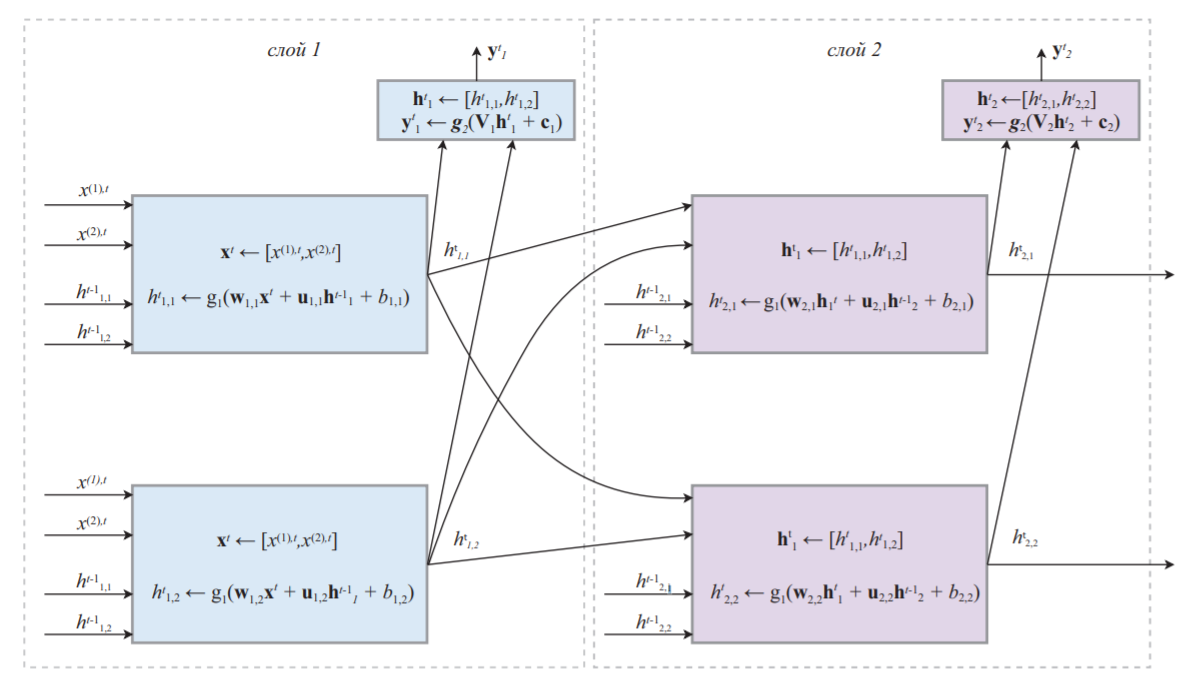
\includegraphics[scale=0.75]{figures/rnn.png}
	\caption{ Первые два слоя в рекуррентной нейронной сети. На вход подается двумерный вектор признаков. Каждый слой имеет два узла }\label{fig:rnn}
\end{figure}

Для обучения моделей RNN используется специальная версия обратного распространения, называемая \emph{обратным распространением во времени}.

Обе функции -- $ \tanh $ и softmax -- страдают проблемой затухания градиентов. Даже если сеть RNN имеет только один или два рекуррентных слоя, из-за последовательного характера входных данных обратное распространение <<развертывает>> сеть с течением времени. С точки зрения вычисления градиента это означает, что чем длиннее входная последовательность, тем глубже полчается развернутая сеть.

Другая проблема, характерая для RNN, заключается в обработке долгосрочных зависимостей. По мере увеличения длины входной последовательности векторы признаков, находящиеся в начале последовательности, постепенно <<забываются>>, потому что состояние всех узлов, которые играют роль памяти сети, в значительной степени зависит от векторов признаков, прочитанных последними.

Наиболее эффективными рекуррентными моделями нейронных сетей, используемые на практике, являются вентильные RNN. К ним относятся сети с \emph{долгой краткосрочной памятью} (LSTM) и сети с вентильными рекуррентными узлами (GRU).

В рекуррентных нейронных сетях операции чтения, записи и стирания информации, хранящейся в каждом узле, контролируются функциями активации, которые принимают значения в диапазоне $ (0, 1) $. Обученная нейронная сеть может <<прочитать>> входную последовательность векторов признаков и на некотором раннем временном шаге $ t $ решить сохранить конкретную информацию о векторах признаков. Эта информация о более ранних векторах признаков может позже использоваться моделью для обработки векторов признаков в конце входной последовательности.

Решение о том, какую информацию хранить и когда разрешать чтение, запись и удаление, принимают узлы. Эти решения принимаются на основе данных и реализуются через идею вентилей. Есть несколько архитектур управляемых узлов. Простая, но эффективная называется \emph{минимальным вентильным узлом} и состоит из \emph{ячейки памяти} и \emph{вентиля забывания}
\begin{align*}
	\tilde{h}^t_{l,u} \leftarrow \tanh (\mathbf{w}_{l,u} \mathbf{x}^t + \mathbf{u}_{l,u} \mathbf{h}_l^{t-1} + b_{l,u}),\\
	\Gamma_{l,u}^t \leftarrow \sigma (\mathbf{m}_{l,u} \mathbf{x}^t + \mathbf{o}_{l,u} \mathbf{h}^{t - 1} + a_{l, u}),\\
	h^t_{l,u} \leftarrow \Gamma^t_{l,u} \tilde{h}_l^t + \big( 1 - \Gamma^t_{l,u}  \big) h_l^{t - 1},\\
	\mathbf{h}_l^t \leftarrow \big[ h_{l,1}^t, \ldots, h_{l, size_l}^t \big],\\
	\mathbf{y}_l^t \leftarrow \mathbf{g}(\mathbf{V}_l \mathbf{h}_l^t + \mathbf{c}_{l,u}),
\end{align*}
где $ \mathbf{g} $ -- функция softmax.

Если вентиль $ \Gamma_{l,u}^t $ близок к 0, тогда ячейка памяти сохраняет значение, полученное на предыдущем временном шаге $ h_l^{t-1} $. Если вентиль $ \Gamma_{l,u}^t $ близок к 1, значение ячейки памяти затирается новым значением $ \tilde{h}^t_{l,u} $.


\section{Приемы работы с библиотекой plotly}

Шаблонный код для JupyterLab
\begin{lstlisting}[
style = ironpython,
numbers = none
]
# ячейка
import numpy as np
import plotly.graph_objs as go
from plotly.offline import (
	download_plotlyjs,
	init_notebook_mode,
	plot,
	iplot,
)
# ячейка
init_notebook_mode(connected=True)
# ячейка
fig = go.Figure()
# ячейка
fig.add_traces([
	go.Scatter(y=np.random.randn(100).cumsum(), name="curve-1"),
	go.Scatter(y=np.random.randn(100).cumsum(), name="curve-2"),
]);
# ячейка
fig.update_layout(
	title=dict(
		text=(
			"<i>Реализации значений переменных</i>"),       
		font=dict(
			family="Arial",
			size=18,
			color="#07689F",
		),
	),
	xaxis_title="<i>Имена переменных</i>",
	yaxis_title="<i>Значение переменной</i>",
	xaxis=dict(
		showline=True,
		showgrid=False,
		showticklabels=True,
		linecolor="rgb(204, 204, 204)",
		linewidth=1.5,
		ticks="outside",
		tickfont=dict(
			family="Arial",
			size=15,
			color="rgb(82, 82, 82)",
		),
	),
	yaxis=dict(
		showgrid=False,
		zeroline=False,
		showline=True,
		showticklabels=True,
		linecolor="rgb(204, 204, 204)",
		linewidth=1.5,
		ticks="outside",
		tickfont=dict(
			family="Arial",
			size=15,
			color="rgb(82, 82, 82)",
		),
	),
	autosize=False,
	margin=dict(
		autoexpand=False,
		l=70,
		r=10,
		t=50,
	),
	showlegend=True,
	plot_bgcolor="white",
	legend_title_text="<i>Имя блока легенды</i>",
	legend=dict(
		orientation="v",
		yanchor="bottom",
		y=0.01,
		xanchor="right",
		x=0.99,
		font=dict(family="Arial", size=12, color="black"),
	),
	font=dict(
		family="Arial",
		size=13,
	),
)
\end{lstlisting}

Если теперь воспользоваться функцией \texttt{plot}, то в текущей директории проекта будет создан \texttt{html}-файл интерактивного графика, который автоматически откроется в браузере
\begin{lstlisting}[
style = ironpython,
numbers = none
]
plot(fig, filename="test-sample.html")
\end{lstlisting}


\section{Приемы работы с библиотекой анализа временных рядов ETNA}

\subsection{Перекрестная проверка на временных рядах}

Перекрестную проверку с расширяющимся окном (или на скользящем окне) в бибилотеке ETNA можно выполнить с помощью метода \verb|.backtest()|. Этот метод возвращает три кадра данных: кадр данных с метриками по каждой тестовой выборке перекрестной проверки, кадр данных с прогнозами и кадр данных с временными метками обучающего и тестового поднаборов данных.

В перекрестной проверке расширяющися окном количество наблюдений, использованных для обучения в каждой итерации, растет с числом итераций, предоставляет все больший объем данных для обучения.

\begin{figure}[h]
	\centering
	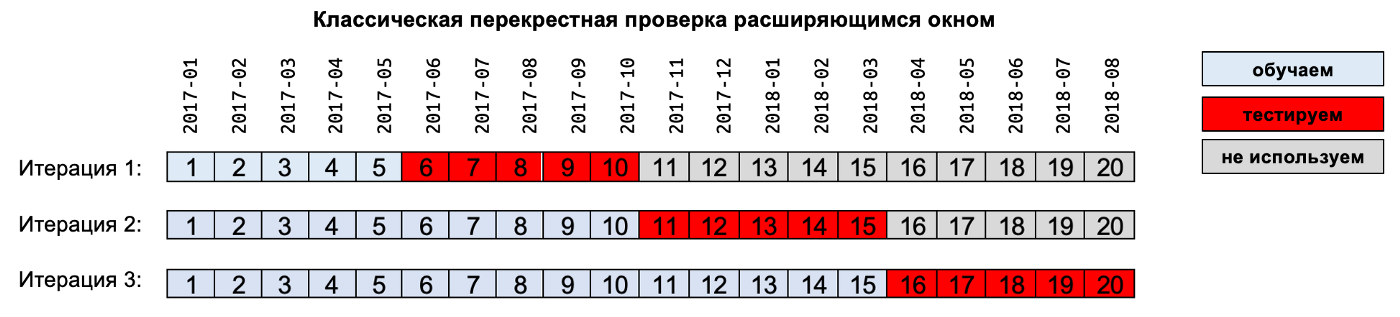
\includegraphics[scale=0.3]{figures/cross_val_ts.png}
	\caption{ Перекрестная проверка на временном ряду \emph{расширяющимся} окном }\label{fig:cross_val_ts}
\end{figure}

Для тестирования мы каждый раз берем совершенно новые более поздние наблюдения. Обучающая выборка прирастает на количество наблюдений, равное горизонту прогнозирования.

При необходимости обучение модели в каждом разбиении можно сделать последовательным, используя в каждой итерации для обучения фиксированное количество наиболее свежих (поздних) наблюдений, предшествующих точке разбиения. Таким образом, в каждой новой итерации мы будем обучаться на более свежих данных, обучающая выборка каждый раз сдвигается вперед по временной оси (обычно на горизонт прогнозирования) и такой способ проверки называют перекрестной проверкой скользящим окном (sliding/rolling window).

\begin{figure}[h]
	\centering
	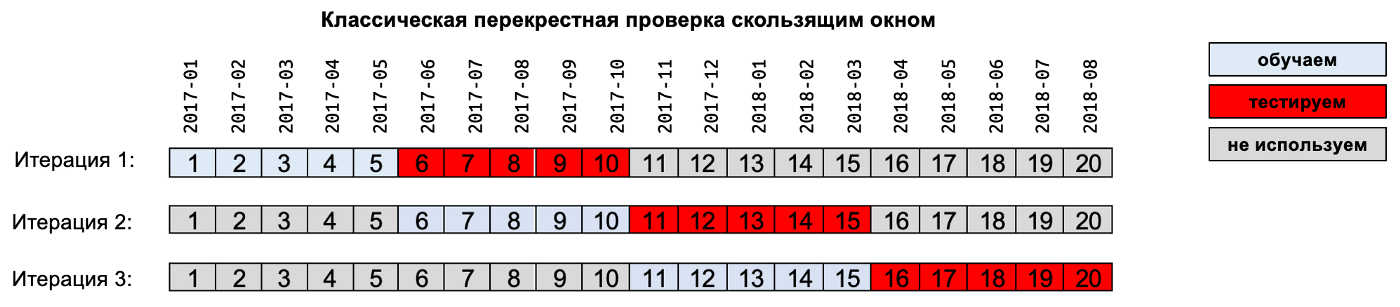
\includegraphics[scale=0.3]{figures/cross_val_rol_ts.png}
	\caption{ Перекрестная проверка \emph{на скользящем} окне }\label{fig:cross_val_rol_ts}
\end{figure}

С каждой итерацией обучающая выборка использует все более свежие наблюдения, при этом для тестирования мы каждый раз берем совершенно новые более поздние наблюдения. Размер обучающей выборки остается неизменным, поэтому в ETNA этот вид проверки назван \verb|constant|.

NB При выполнении перекрестной проверки для временных рядов полезно помнить ряд правил:
\begin{itemize}
	\item Размер тестовой выборки, как правило, определяется горизонтом прогнозирования, а тот в свою очередь определяется бизнес-требования. Если вы предсказываете на 14 дней вперед, то и тестовая выборка должна включать 14 более поздних наблюдений.
	
	\item Размер тестовой выборки остается постоянным. Это значит, что метрики качества, полученные в результате вычислений прогнозов каждой обученной модели по тестовому набору, будут последовательны и их можно объединять и сравнивать.
	
	\item Размер обучающей выборки не может быть меньше тестовой выборки.
	
	\item Если данные содержат сезонность, обучающая выборка должна содержать не менее двух полных сезонных циклов (правило $ 2L $, где $ L $ -- количество периодов в полном сезонном цикле, необходимое для инициализации параметров некоторых моделей, например, для вычисления исходного значения тренда в модели тройного экспонециального сглаживания), учитывая уменьшение длины ряда при выполнении процедур обычного и сезонного дифференциирования.
	
	\item Если применяются переменные -- лаги, разности на лагах, скользящие статистики, то каждый раз для получения значений в тестовой выборке используются только данных обучающей выборки.
\end{itemize}

Перекрестную проверку расширяющимся окном можно модифицировать так, чтобы обучающая выборка прирастала на количество наблюдений меньше горизонта прогнозирования и тогда в тестовую выборку попадут наблюдения, уже попадавшие в тестовую выборку на предыдущей итерации. Это позволяет управлять скоростью обновления модели, лучше выявлять аномальные, нетипичные наблюдения, которые плохо предсказываются, точнее определить момент ухудшения качества модели.

\begin{figure}[h]
	\centering
	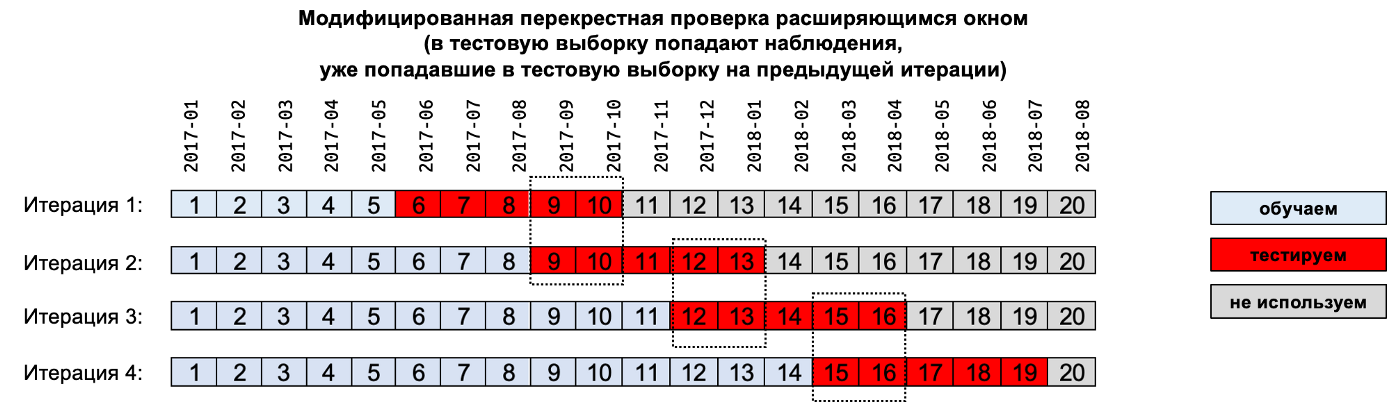
\includegraphics[scale=0.3]{figures/cross_val_expand_ts.png}
	\caption{ Модфицированная перекрестная проверка расширяющимся окном }\label{fig:cross_val_expand_ts}
\end{figure}

Перекрестную проверку скользящим окном тоже можно модифицировать так, чтобы обучающая выборка сдвигалась вперед не на весь горизонт прогнозирония, а на половину или на треть, и тогда в тестовую выборку попадут наблюдения, уже попадавшие в тестовую выборку на предыдущей итерации. Это позволяет управлять скоростью обновления модели, лучше выявлять аномальные, нетипичные наблюдения, которые плохо предсказываются, точнее определять момент ухудшения качества модели.

\begin{figure}[h]
	\centering
	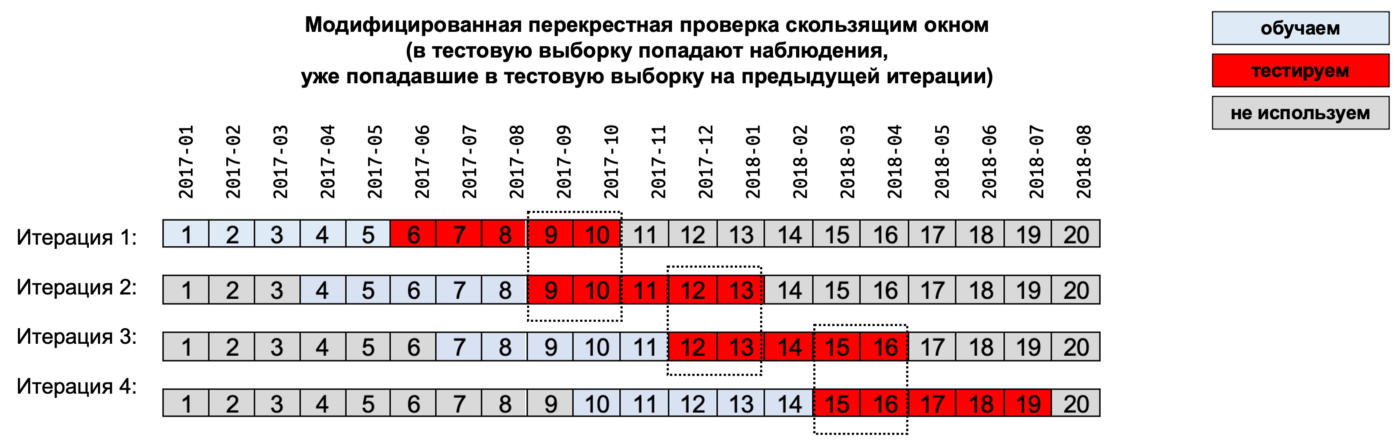
\includegraphics[scale=0.3]{figures/cross_val_rol_modif_ts.png}
	\caption{ Модфицированная перекрестная проверка скользящим окном }\label{fig:cross_val_rol_modif_ts}
\end{figure}

Однако, в библиотеке ETNA и библиотеке scikit-learn с помощью класса TimeSeriesSplit нельзя корректно реализовать вышеописанные модификации.

При использовании перекрестной проверки расширяющимся окном модель в большей степени нацелена на обнаружение глобальных паттернов и менее склонна к изменениям, т.е. более консервативна. При использовании перекрестной проверки скользящим окном используется меньше данных, модель быстрее меняет поведение, т.е. менее консервативна. В ситуации, когда вы уверены, что процесс, генерирующий данные, изменился или неоднократно менялся в течение периода, охватывающего исторические данные, используйте перекрестную проверку скользящим окном.

Для рынков товаров с низкой вовлеченностью (товаров повседневного спроса), в ситуации, когда вы уверены или у вас есть доказательства, что процесс, генерирующий данные, остается неизменным или претерпевает несущественные изменения, перекрестная проверка расширяющимся окном может быть более полезна.

\remark{
Важно помнить, что во временных рядах \emph{перекрестная проверка}, которую вы применяете, является \emph{прообразом} вашей \emph{производственной системы}. Если вы применяли для валидации перекрестную проверку расширяющимся окном, то и в производстве вы должны обучать модель на обучающей выборке возрастающего объема и обновлять в том же темпе, что обновляли в ходе перекрестной проверки (на весь горизонт прогнозирования, на половину горизонта и т.д.)
}

Наконец, поскольку в рамках перекрестной проверки расширяющимся окном мы на каждой итерации обучаем модель на выборке все большего объема, при использовании моделей на основе градиентного бустинга это может потребовать коррекции темпа обучения, количества деревьев и максимальной глубины. 

\subsection{CatBoost. Базовая модель с конструированием признаков}

В ETNA есть два класса-обертки над классом \texttt{CatboostRegressor}: \texttt{CatBoostModePerSegment} и \texttt{CatBoostModelMultiSegment}. Разница заключается в том, что класс \texttt{CatBoostModelPerSegment} обучает отдельную модель для каждого сегмента, а класс \texttt{CatBoostModelMultiSegment} -- одну модель для всех сегментов.

Для создания признаков можно использовать классы-трансформеры:
\begin{itemize}
	\item \texttt{LagTransform} для генерации лагов,
	
	\item \texttt{MeanTransform} для вычисления скользящего среднего по заданному окну.
\end{itemize}

\remark{
Ширину окна $ w $ для скользящих статистик \emph{рекомендуется} задавать равной или превышающей горизонт прогнозирования $ h $, т.е. $ w \geqslant h $. То же относится и к лагам. Порядок лага $ lag $ должен быть равен или превышать горизонт прогнозирования, т.е. $ lag \geqslant h $. В противном случае признаки тествого поднабора данных (построенные на лагах с  порядком меньшим горизонта прогнозирования), будут использовать значения целевой переменной из тестового поднабора данных (утечка)
}

С помощью параметра \verb|in_column| класса-трансформера задаем переменную, которую нужно преобразовать или на основе которой нужно создать признаки (по умолчанию этой переменной будет переменная \texttt{target}). С помощью параметра \verb|out_column| (этот параметр есть у всех классов-трансформеров, создающих признаки) можно задать имена генерируемых переменных.

Для более надежной оценки качества модели следует восопользоваться \emph{перекрестной проверкой расширяющимся окном} с помощью класса \texttt{Pipeline}.

Создадим список преобразований. В данном случае он включать формирование лагов и скользящего среднего на каждой итерации перекрестной проверки.

\begin{lstlisting}[
style = ironpython,
numbers = none
]
lags = LagTransform(in_column="target", lags=list(range(8, 24, 1)), out_column="lag")
mean8 = MeanTransform(in_column="target", window=8, out_column="mean8")
transforms = [lags, mean8]
\end{lstlisting}

Теперь создаем конвейер для выполнения перекрестной проверки расширяющимся окном, передав в него модель, список процедур формирования признаков (лагов и скользящего среднего) и горизонт прогнозирования
\begin{lstlisting}[
style = ironpython,
numbers = none
]
model = CatBoostModelMultiSegment()
model.fit(train_ts)

pipeline = Pipeline(
    model=model,
    transforms=transforms,
    horizon=HORIZON,
)
# перекрестная проверка расширяющимся окном
metrics_df, _, _ = pipeline.backtest(
    ts=ts,
    mode="expand",
    metrics=[smape],
)
\end{lstlisting}

Класс \texttt{Pipeline} можно использовать для перекрестной проверки сразу нескольких моделей
\begin{lstlisting}[
style = ironpython,
numbers = none
]
# задаем конвейер преобразований для модели наивного прогноза
naive_pipeline = Pipeline(
    model=NaiveModel(lag=12), transforms=[], horizon=HORIZON)
# задаем конвейер преобразований для Prophet
prophet_pipeline = Pipeline(
    model=ProphetModel(), transforms=[], horizon=HORIZON
)
# задаем конвейер преобразований для CatBoost
catboost_pipeline = Pipeline(
    model=CatBoostModelMultiSegment(),
    transforms=[LagTransform(lags=[8, 9, 10, 11, 12], 
    in_column='target')],
    horizon=HORIZON
)
# задаем список имен конвейеров
pipeline_names = ['naive', 'prophet', 'catboost']
# задаем список конвейеров
pipelines = [naive_pipeline, prophet_pipeline, catboost_pipeline]
# задаем пустой список метрик
metrics = []
# записываем метрики в список
for pipeline in pipelines:
    metrics.append(
        pipeline.backtest(
        ts=ts, metrics=[MAE(), MSE(), SMAPE(), MAPE()], 
        n_folds=3, aggregate_metrics=True
    )[0].iloc[:, 1:]
)

# конкатенируем метрики
metrics = pd.concat(metrics)
# в качестве индекса используем список имен конвейеров
metrics.index = pipeline_names
\end{lstlisting}

С помощью класса \texttt{VotingEnsemble} можно выполнить обучение и перекрестную проверку \emph{ансамбля моделей}. Веса моделей можно задавать с помощью параметра \texttt{weights}
\begin{lstlisting}[
style = ironpython,
numbers = none
]
# создаем экземпляр класса VotingEnsemble
voting_ensemble = VotingEnsemble(pipelines=pipelines, 
weights=[1, 2, 4], 
n_jobs=4)
# получаем метрики
voting_ensamble_metrics = voting_ensemble.backtest(
    ts=ts,
    metrics=[MAE(), MSE(), SMAPE(), MAPE()], 
    n_folds=3,
    aggregate_metrics=True,
    n_jobs=2
)[0].iloc[:, 1:]
voting_ensamble_metrics.index = ['voting ensemble']
\end{lstlisting}

С помощью класса \texttt{StackingEnsemble} можно выполнить \emph{стекинг}. Мы прогнозируем будущее, используя метамодель (линейную регрессию по умолчанию) для объединения прогнозов моделей в списке конвейеров. С помощью параметров \verb|final_model| можно задать метамодель. С помощью \verb|features_to_use| можно задавать признаки для метамодели
\begin{itemize}
	\item \texttt{None}: метамодель в качестве признаков может использовать прогнозы моделей конвейеров,
	
	\item \texttt{List}: прогнозы моделей конвейеров плюс признаки из списка (в виде строковых значений),
	
	\item \texttt{"all"}: все доступные признаки.
\end{itemize}

С помощью параметра \texttt{cv} задаем количество тестовых выборок перекрестной выборки (используем не для оценки моделей, а для получения прогнозов, которые станут у нас потом признаками).

Под капотом происходит примерно следующее. Допустим, запустили перекрестную проверку расширяющимся окном, получили 5 тестовых выборок, прогнозы каждой из модели конвейера в 5 тестовых выбоках стали признаками. Затем снова запускаем проверку расширяющимся окном, по этим признакам строим метамодель -- линейную регрессию, берем прогнозы в 3 тестовых выборках и усредняем
\begin{lstlisting}[
style = ironpython,
numbers = none
]
# создаем экземпляр класса StackingEnsemble,
# признаки - прогнозы конвейеров
stacking_ensemble_unfeatured = StackingEnsemble(
    features_to_use='None', pipelines=pipelines, 
    n_folds=10, n_jobs=4)
# выполняем стекинг
stacking_ensamble_metrics = stacking_ensemble_unfeatured.backtest(
    ts=ts, metrics=[MAE(), MSE(), SMAPE(), MAPE()], n_folds=3, 
    aggregate_metrics=True, n_jobs=2)[0].iloc[:, 1:]
stacking_ensamble_metrics.index = ['stacking ensemble']
stacking_ensamble_metrics
\end{lstlisting}

\subsection{Пользовательские классы для вычисления скользящих статистик}

Можно писать свои собственные классы для вычисления скользящих статистик и обучения моделей. Допустим, мы хотим использовать не только скользящие средние, но и скользящие средние абсолютные отклонения
\begin{lstlisting}[
style = ironpython,
numbers = none
]
# пишем класс MadTransform, вычисляющий скользящие
# средние абсолютные отклонения
class MadTransform(WindowStatisticsTransform):
    """
    MadTransform вычисляет среднее абсолютное отклонение
    (mean absolute deviation - mad) для заданного окна.
    """
		def __init__(
			self,
			in_column: str,
			window: int,
			seasonality: int = 1,
			min_periods: int = 1,
			fillna: float = 0,
			out_column: Optional[str] = None
		):
		"""
		Параметры
		----------
		in_column: str
		имя обрабатываемого столбца
		window: int
		ширина окна для агрегирования
		out_column: str, optional
		имя результирующего столбца. Если не задано, 
		используем __repr__()
		seasonality: int
		коэффициент сезонности
		min_periods: int
		Минимальное количество наблюдений в окне 
		для агрегирования
		fillna: float
		значение для заполнения значений NaN
		"""
		self.in_column = in_column
		self.window = window
		self.seasonality = seasonality
		self.min_periods = min_periods
		self.fillna = fillna
		self.out_column = out_column
		super().__init__(
		window=window,
		in_column=in_column,
		seasonality=seasonality,
		min_periods=min_periods,
		out_column=self.out_column 
		if self.out_column is not None 
		else self.__repr__(),
		fillna=fillna,
	)
	def _aggregate_window(
		self, series: pd.Series
	) -> float:
		"""Вычисляет mad для серии."""
		tmp_series = self._get_required_lags(series)
		return tmp_series.mad(**self.kwargs)
\end{lstlisting}

Теперь предположим, мы хотим использовать LightGBM вместо CatBoost. Нам понадобиться класс LGBRegressor и базовые классы библиотеки ETNA \texttt{Model} и \texttt{PerSegmentModel}.

Сначала надо написать ядро -- внутренний класс \verb|_LBGMModel|, в котором используется \texttt{LGBMRegressor}. Символ нижнего подчеркивания указывает, что данный класс будет использоваться внутри других классов. У класса \verb|_LGBModel| будут два метода \texttt{fit()} и \texttt{predict()}.

\begin{lstlisting}[
style = ironpython,
numbers = none
]
# пишем ядро - внутренний класс _LGBMModel,
# внутри - класс LGBMRegressor
class _LGBMModel:
	def __init__(
		self,
		boosting_type='gbdt',
		num_leaves=31,
		max_depth=-1,
		learning_rate=0.1,
		n_estimators=100,
		**kwargs
	):
		self.model=LGBMRegressor(
			boosting_type=boosting_type,
			num_leaves=num_leaves,
			max_depth=max_depth,
			learning_rate=learning_rate,
			n_estimators=n_estimators,
			**kwargs
		)
	def fit(self, df: pd.DataFrame):
		features = df.drop(columns=['timestamp', 'target'])
		target = df['target']
		self.model.fit(X=features, y=target)
		return self
		
	def predict(self, df: pd.DataFrame):
		features = df.drop(columns=['timestamp', 'target'])
		pred = self.model.predict(features)
		return pred
\end{lstlisting}

Вспомним, что мы можем строить отдельную модель для каждого сегмента и одну модель для всего набора (т.е. всех сегментов). Значит мы можем написать два класса. Начнем с класса, который будет строить отдельную модель для каждого сегмента. Назовем его \texttt{LGBModelPerSegment}. Для этого воспользуемся наследованием, нам понадобится базовый класс \texttt{PerSegmentModel}

\begin{lstlisting}[
style = ironpython,
numbers = none
]
# пишем класс LGBMModelPerSegment, который строит 
# отдельную модель LGBM для каждого сегмента
class LGBMModelPerSegment(PerSegmentModel):
	def __init__(
		self,
		boosting_type='gbdt',
		num_leaves=31,
		max_depth=-1,
		learning_rate=0.1,
		n_estimators=100,
		**kwargs
	):
		self.kwargs = kwargs
		model = _LGBMModel(
			boosting_type=boosting_type,
			num_leaves=num_leaves,
			max_depth=max_depth,
			learning_rate=learning_rate,
			n_estimators=n_estimators,
			**kwargs
		)
		super(LGBMModelPerSegment, self).__init__(
			base_model=model)
\end{lstlisting}

Теперь напишем класс, который будет строить одну модель для всех сегментов. Назовем его \texttt{LGBModelMultiSegment}. Для этого вновь воспользуемся наследованием, нам понадобится базовый класс \texttt{Model}

\begin{lstlisting}[
style = ironpython,
numbers = none
]
# пишем класс LGBMModelMultiSegment, который строит 
# одну модель LGBM для всех сегментов
class LGBMModelMultiSegment(Model):
	def __init__(
		self,
		boosting_type='gbdt',
		num_leaves=31,
		max_depth=-1,
		learning_rate=0.1,
		n_estimators=100,
		**kwargs
	):
		self.kwargs = kwargs
		super(LGBMModelMultiSegment, self).__init__()
		self._base_model=_LGBMModel(
			boosting_type=boosting_type,
			num_leaves=num_leaves,
			max_depth=max_depth,
			learning_rate=learning_rate,
			n_estimators=n_estimators,
			**kwargs
		)
		
	def fit(self, ts: TSDataset):
		# превращаем TSDataset в датафрейм pandas
		# с плоским индексом
		df = ts.to_pandas(flatten=True)
		df = df.dropna()
		df = df.drop(columns='segment')
		self._base_model.fit(df=df)
		return self
		
	def forecast(self, ts: TSDataset):
		result_list = list()
		# собираем новый датафрейм с помощью self._forecast_segment
		# из базового класса
		for segment in ts.segments:
			segment_predict = self._forecast_segment(
				self._base_model, segment, ts)
			result_list.append(segment_predict)
			
		result_df = pd.concat(result_list, ignore_index=True)
		result_df = result_df.set_index(['timestamp', 'segment'])
		
		df = ts.to_pandas(flatten=True)
		df = df.set_index(['timestamp', 'segment'])
		# заменяем пропуски прогнозами
		df = df.combine_first(result_df).reset_index()
		df = TSDataset.to_dataset(df)
		ts.df = df
		# выполняем обратные преобразования
		ts.inverse_transform()
		
		return ts
\end{lstlisting}

Аналогично можно реализовать XGBoost в ETNA. Пишем класс \verb|_XGBModel|
\begin{lstlisting}[
style = ironpython,
numbers = none
]
class _XGBModel:
    def __init__(
        self,
        booster="gbtree",
        max_depth=3,
        learning_rate=0.1,
        n_estimators=100,
        **kwargs,
    ):
        self.model=XGBRegressor(
            booster=booster,
            max_depth=max_depth,
            learning_rate=learning_rate,
            n_estimators=n_estimators,
            **kwargs,
        )
        
    def fit(
        self,
        df: pd.DataFrame,
    ):
        features = df.drop(columns=["timestamp", "target"])
        for col in features.columns.tolist():
            features[col] = features[col].astype("category").cat.codes
        target = df["target"]
        self.model.fit(X=features, y=target)
        return self
        
    def predict(
        self,
        df: pd.DataFrame,
    ):
        features = df.drop(columns=["timestamp", "target"])
        for col in features.columns.tolist():
            features[col] = features[col].astype("category").cat.codes
        pred = self.model.predict(features)
        return pred
\end{lstlisting}

Пишем классы \texttt{XGBModePerSegment} и \texttt{XGBModelMultiSegment}
\begin{lstlisting}[
style = ironpython,
numbers = none
]
# пишем класс XGBModelPerSegment, который строит 
# отдельную модель XGB для каждого сегмента
class XGBModelPerSegment(PerSegmentModel):
	def __init__(
		self,
		booster='gbtree',
		max_depth=3,
		learning_rate=0.1,
		n_estimators=200,
		**kwargs
	):
	self.kwargs = kwargs
	model = _XGBModel(
		booster=booster,
		max_depth=max_depth,
		learning_rate=learning_rate,
		n_estimators=n_estimators,
		**kwargs
	)
	super(XGBModelPerSegment, self).__init__(
		base_model=model)
		
# пишем класс XGBModelMultiSegment, который строит 
# одну модель XGB для всех сегментов
class XGBModelMultiSegment(Model):
	def __init__(
		self,        
		booster='gbtree',
		max_depth=3,
		learning_rate=0.1,
		n_estimators=100,
		**kwargs
	):
		self.kwargs = kwargs
		super(XGBModelMultiSegment, self).__init__()
		self._base_model=_XGBModel(
			booster=booster,
			max_depth=max_depth,
			learning_rate=learning_rate,
			n_estimators=n_estimators,
			**kwargs
	)
	
	def fit(self, ts: TSDataset):
		# превращаем TSDataset в датафрейм pandas
		# с плоским индексом
		df = ts.to_pandas(flatten=True)
		df = df.dropna()
		df = df.drop(columns='segment')
		self._base_model.fit(df=df)
		return self
		
	def forecast(self, ts: TSDataset):
		result_list = list()
		# собираем новый датафрейм с помощью 
		# self._forecast_segment 
		# из базового класса
		for segment in ts.segments:
			segment_predict = self._forecast_segment(
				self._base_model, segment, ts)
			result_list.append(segment_predict)
			
		result_df = pd.concat(result_list, ignore_index=True)
		result_df = result_df.set_index(['timestamp', 'segment'])
		
		df = ts.to_pandas(flatten=True)
		df = df.set_index(['timestamp', 'segment'])
		# заменяем пропуски прогнозами
		df = df.combine_first(result_df).reset_index()
		df = TSDataset.to_dataset(df)
		ts.df = df
		# выполняем обратные преобразования
		ts.inverse_transform()

		return ts
\end{lstlisting}

\remark{
Порядок лагов не должен быть меньше длины горизонта! Потому как в противном случае, признаки тествого поднабора данных, построенные на лагах, будут использовать информацию из целевой переменной тестового поднабора данных (утечка!)
}

Таким образом, необходимо создаватвь лаговые переменные так, чтобы они не проникали в тестовый набор. Лаги вида $ L_{t-k} $ лучше создавать так, чтобы $ k $ был равен или превышал горизонт прогнозирования (\pic{fig:lags}). Впрочем, допускается создание лагов, у которых порядок будет меньше длины горизонта прогнозирования, но тогда значения зависимой переменной в тестовой выборке нужно заменить на значение NaN. Если лаг и залезет в тест, ему ничего не останется, как использовать значение NaN, таким образом, в тесте появится значение NaN. В таком случае, чем больше горизонт прогнозирования будет превышать порядок лага, тем больше пропусков будет в тесте.

На практике для избежания утечки данных при вычислении лагов (а также скользящих и расширяющихся статистик) поступают двумя способами:
\begin{itemize}
	\item значения зависимой переменной в наблюдениях исходного набора, которые будут соответствовать будущей тестовой выборке (набору новых данных), заменяют значениями NaN,
	
	\item берем обучающую выборку и удлиняем ее на длину горизонта прогнозирования, зависимая переменная в наблюдениях, соответсвтующих новым временным меткам (т.е. в тестовой выборке/наборе новых данных) получает значения NaN.
\end{itemize}

В обоих случаях мы формирум защиту от утечки при вычислении лагов в тестовой выборке / наборе новых данных.

\begin{figure}[h]
	\centering
	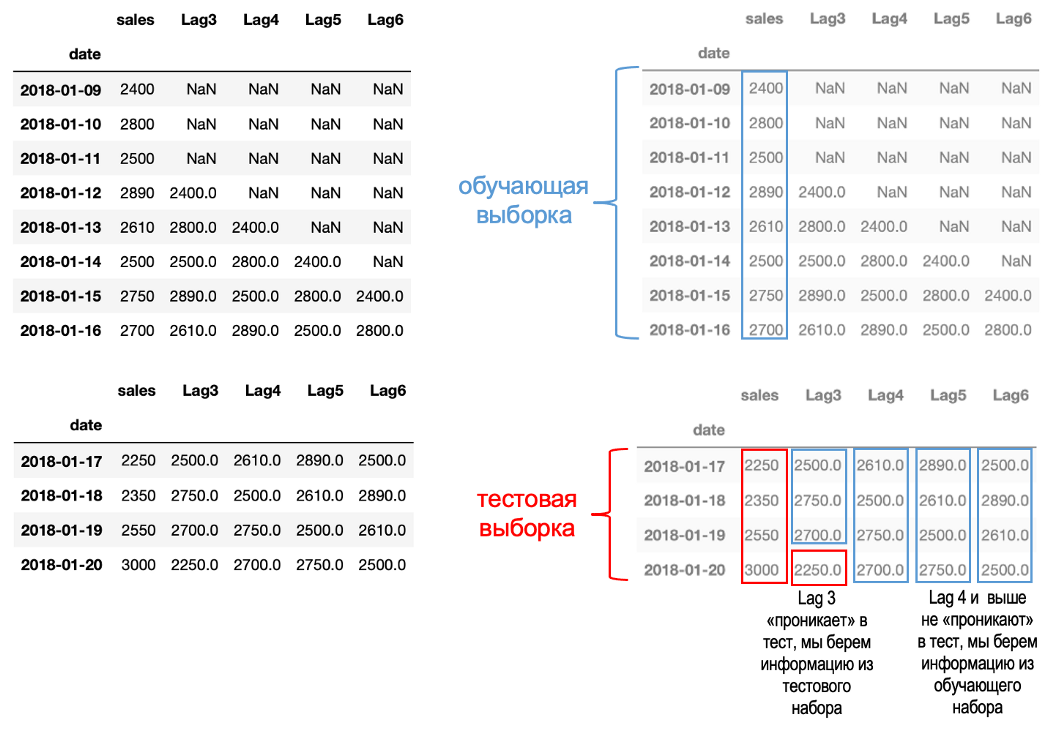
\includegraphics[scale=0.4]{figures/lags.png}
	\caption{ Лаги, у которых порядок равен горизонту прогнозирования или превышает его, не используют тестовую выборку }\label{fig:lags}
\end{figure}



Теперь создадим лаги, скользящее среднее, скользящее среднее абсолютное отклонение, обучим модель \texttt{LGBMModelMultiSegment}, получим прогнозы и визуализируем их
\begin{lstlisting}[
style = ironpython,
numbers = none,
]
# создаем экземпляр класса LagTransform для генерации лагов,
# с помощью in_column задаем переменную, на основе которой
# генерируем лаги, мы будем генерировать лаги порядка от 8 до 23, 
# порядок лагов не должен быть меньше длины горизонта
lags = LagTransform(in_column='target', 
				lags=list(range(8, 24, 1)), 
				out_column='lag')
# создаем экземпляр класса MeanTransform для вычисления 
# скользящего среднего по заданному окну
mean8 = MeanTransform(in_column='target', 
				window=8, 
				out_column='mean8')
# создаем экземпляр класса MadTransform для вычисления 
# среднего абсолютного отклонения по заданному окну
mad8 = MadTransform(in_column='target',
				window=8, 
				out_column='mad8')
# добавляем лаги, mean8, mad8 в обучающую выборку
train_ts.fit_transform([lags, mean8, mad8])
# создаем экземпляр класса LGBMModelPerSegment
model = LGBMModelPerSegment()
# обучаем модель
model.fit(train_ts)
# формируем тестовый набор
future_ts = train_ts.make_future(HORIZON)
# получаем прогнозы
forecast_ts = model.forecast(future_ts)
# оцениваем качество прогнозов
smape(y_true=test_ts, y_pred=forecast_ts)
\end{lstlisting}

\subsection{Работа с несколькими временными рядами}

Прогнозирование нескольких временных рядов. Загрузим набор, в котором каждому сегменту соответствует свой временной ряд
\begin{lstlisting}[
style = ironpython,
numbers = none	
]
original_df = pd.read_csv("data.csv")
original_df.head()

df = TSDataset.to_dataset(original_df)
\end{lstlisting}

Вновь воспользуемся моделью CatBoost с помощью класса CatBoostModelMultiSegment. Перед построением модели выполним некоторые преобразования и создадим новые признаки для наших рядов.

Нам понадобятся следующие классы-трансформеры:
\begin{itemize}
	\item класс \texttt{LogTransform} для логарифмирования и экспонецирования перерменной (логарифмирование позволяет сгладить негативное влияние выборосов объективной природы, помогает выделить тренд),
	
	\item \texttt{LinearTrendTransform} для прогнозирования тренда, удаления тренда из данных и добавления тренда к прогнозам (это необходимо для деревьев решений и для ансамблей деревьев решений, \underline{\emph{не умещющих экстраполировать}}),
	
	\item \texttt{LagTransform} для генерации лагов,
	
	\item \texttt{DateFlagsTransform} для генерации признаков на основе дат -- порядковый номер дня недели, порядковый номер дня месяца, порядковый номер недели в месяце и пр.,
	
	\item \texttt{MeanTransform} для вычисления скользящего среднего по заданному окну.
\end{itemize}

Сначала выполним логарифмирование зависимой переменной, а затем вычтем из нее тренд. Потом на основе пролагрифмированной зависимой переменной с удаленным трендом мы создадим лаги и скользящие средние, добавим календарные признаки.

\begin{lstlisting}[
style = ironpython,
numbers = none
]
# создаем экземпляр класса LogTransform для логарифмирования 
# и экспоненцирования зависимой переменной
log = LogTransform(in_column='target')

# создаем экземпляр класса LinearTrendTransform 
# для прогнозирования тренда, удаления тренда из 
# данных и добавления тренда к прогнозам
trend = LinearTrendTransform(in_column='target')

# создаем экземпляр класса SegmentEncoderTransform 
# для кодирования меток сегментов целочисленными 
# значениями в лексикографическом порядке (LabelEncoding): 
# сегменты a, b, c, d получат значения 0, 1, 2, 3
seg = SegmentEncoderTransform()

# создаем экземпляр класса LagTransform 
# для генерации лагов (c лага 31 по лаг 95)
lags = LagTransform(in_column='target', 
	lags=list(range(31, 96, 1)), 
	out_column='lag')
	
# создаем экземпляр класса DateFlagsTransform для 
# генерации признаков на основе дат - порядковый 
# номер дня недели, порядковый номер дня месяца,
# порядковый номер недели в месяце, порядковый 
# номер недели в году, порядковый номер месяца 
# в году, индикатор выходных дней
d_flags = DateFlagsTransform(day_number_in_week=True,
	day_number_in_month=True,
	week_number_in_month=True,
	week_number_in_year=True,
	month_number_in_year=True,
	special_days_in_week=[5, 6], 
	out_column='datetime')
	
# создаем экземпляр класса MeanTransform для вычисления 
# скользящего среднего по заданному окну
mean30 = MeanTransform(in_column='target', 
	window=30, 
	out_column='mean30')
\end{lstlisting}

Разбиваем набор (наш объект TSDataset) на обучающую и тестовую выборки с учетом временной структуры. Здесь горизонт прогнозирования сосавит 31 день
\begin{lstlisting}[
style = ironpython,
numbers = none
]
# разбиваем набор на обучающую и тестовую выборки 
# с учетом временной структуры
train_ts, test_ts = ts.train_test_split(
    train_start="2019-01-01",
    train_end="2019-11-30",
    test_start="2019-12-01",
    test_end="2019-12-31",
)

# выполняем преобразования набора
train_ts.fit_transform([
	log,  # логарифмируем
	trend,  # удаляем тренд
	lags,  # вычисляем лаги
	d_flags,  # вычисляем признаки на основе дат
	seg,  # кодируем метки сегментов
	mean30  # вычисляем скользящее среднее
])
\end{lstlisting}

Задаем явно горизонт в 31 день, обучаем модель CatBoost, оцениваем качество прогнозов и визуализируем прогнозы. Кроме того, не забываем выполнить обратные преобразования (добавление тренда, экспонецирование зависимой переменной) с помощью метода \texttt{.inverse\_transform()} для обучающего набора для правильной визуализации значений зависимой переменной в обучающей выборке.

\begin{lstlisting}[
style = ironpython,
numbers = none
]
# задаем горизонт прогнозирования
HORIZON = 31
# создаем экземпляр класса CatBoostModelMultiSegment
model = CatBoostModelMultiSegment()
# обучаем модель CatBoost
model.fit(train_ts)
# формируем набор, для которого нужно получить прогнозы,
# длина набора определяется горизонтом прогнозирования
future_ts = train_ts.make_future(HORIZON)

# получаем прогнозы
forecast_ts = model.forecast(future_ts)

# оцениваем качество прогнозов
smape(y_true=test_ts, y_pred=forecast_ts)
\end{lstlisting}

Выполняем обратное преобразование для обратной выборки (добавляем тренд, делаем экспоненцирование переменной \texttt{target})
\begin{lstlisting}[
style = ironpython,
numbers = none
]
train_ts.inverse_transform()
plot_forecast(forecast_ts, test_ts, train_ts, n_train_sample=20)
\end{lstlisting}

Для более надежной оценки качества модели \texttt{CatBoost} воспользуемся \emph{перекрестной проверкой расширяющимся окном}
\begin{lstlisting}[
style = ironpython,
numbers = none
]
pipe = Pipeline(
    model=model,
    transform=[
        log,
        trend,
        seg,
        lags,
        d_flags,
        mean30,
    ],
    horizon=HORIZON,
)
metrics, forecast, info = pipe.backtest(ts, [smape], aggregate_metrics=True)
\end{lstlisting}

Ансамбль бустингов
\begin{lstlisting}[
style = ironpython,
numbers = none,
]
transforms = [log, trend, seg, lags, d_flags, mean30]
catboost_pipeline = Pipeline(
    model=CatBoostModelMultiSegment(),
    transforms=transforms,
    horizon=HORIZON
)

lightgbm_pipeline = Pipeline(
    model=LGBMModelMultiSegment(),
    transforms=transforms,
    horizon=HORIZON
)

xgboost_pipeline = Pipeline(
    model=XGBModelMultiSegment(learning_rate=0.2, n_estimators=500, max_depth=1),
    transforms=transforms,
    horizon=HORIZON
)

pipeline_names = ["catboost", "lightgbm", "xgboost"]
pipelines = [catboost_pipeline, lightgbm_pipeline, xgboost_pipeline]

voting_ensemble = VotingEnsemble(
    pipelines=pipelines,
    weight=[1, 1, 2],
    n_jobs=1
)

metrics, forecast, _ = voting_ensemble.backtest(
    ts=ts, metrics=[SMAPE()], n_folds=3, aggregate_metrics=True, n_jobs=1
)
\end{lstlisting}

Заметим, что скользящее среднее используется не только для конструирования признаков, но и в качестве прогнозной модели (когда прогноз -- скользящее среднее $ n $ последних наблюдений), а также для сглаживания выборосов, краткосрочных колебаний и более четкого выделения долгосрочных тенденций в ряде данных.

\section{Генерация признаков и кодирование категориальных признаков}

Процесс создания признакового пространства зависит от модели, которую будем использовать:
\begin{itemize}
	\item OHE-кодирование предпочтительнее для линейных моделей,
	
	\item умное кодирование категорий -- для деревьев,
	
	\item выбросы можно не удалять для робастной модели.
\end{itemize}

Если в тестовом наборе данных присутствуют категории, которых не было в обучающем наборе данных, то нужно принять решение о том, как их кодировать. Например, категорию из нового набора данных можно отнести к самомой опасной категории из тех, категорий, которые присутствуют в обучающем наборе данных.

Еще категории можно кодировать по разным признакам.

Можно кодировать признаки по мощности (Count Encoding): сколько раз каждая уникальная категория встречалась в категориальном признаке. Проблема в том, что некоторые категории могут встречаться одинаковое количество раз (коллизия). Чтобы различать такие категории можно добавить шум, т.е. $ count + \varepsilon $. Мелкие и новые категории объединяют в одну.

Кодирование по мощности можно использовать, если требуется быстро решить задачу.

\subsection{Кодирование одного категориального признака по другому категориальному признаку с помощью сингулярного разложения}

Если матрица признакового описания объекта состоит только из категориальных признаков, то можно кодировать один признак на основе другого
\begin{lstlisting}[
style = ironpython,
numbers = none
]
from numpy.linalg import svd

def code_factor(data, cat_feature, cat_feature2):
    """
    Кодирование признака на основе другого признака
    """
    ct = pd.crosstab(data[cat_feature], data[cat_feature2])
    u, _, _ = svd(ct.values)
    coder = dict(zip(ct.index, u[:, 0]))  # берем только первый сингулярный вектор
    
    return data[cat_feature].map(coder)
\end{lstlisting}

Сингулярное разложение (Singular Value Decomposition, SVD) -- декомпозиция вещественной матрицы с целью ее приведения к каноническому виду. Сингулярное разложение является удобным методом при работе с матрицами. Оно показывает геометрическую структуру матрицы и позволяет наглядно представить имеющиеся данные. В числе прочего SVD позволяет вычислять обратные и псевдообратные матрицы большого размера, что делает его полезным инструментом при решении задач регрессионного анализа.

\remark{
В числе прочего с помощью сингулярного разложения можно решать задачи обращения или пвседообращения матриц большого размера
}

Для любой вещественной $ (n \times n) $-матрицы $ A $ существуют две вещественные ортогональные $ (n \times n) $-матрицы $ U $ и $ V $ такие, что
\begin{align*}
	\Lambda = U^{T} A V,
\end{align*}
где $ \Lambda $ -- диагональная матрица.

Матрицы $ U $ и $ V $ выбираются так, чтобы диагональные элементы матрицы $ A $ имели вид
\begin{align*}
	\lambda_1 \geqslant \lambda_2 \geqslant \ldots \geqslant \lambda_r > \lambda_{r + 1} = \lambda_n = 0,
\end{align*}
где $ r $ -- ранг матрицы $ A $.

В частности, если $ A $ невырождена (то есть существует обратная матрица $ A^{-1}, \det A \neq 0 $), то
\begin{align*}
	\lambda_1 \geqslant \lambda_2 \geqslant \ldots \geqslant \lambda_n > 0.
\end{align*}

\underline{Столбцы} матриц $ U $ и $ V $ называются соответсвенно \emph{левыми} и \emph{правыми сингулярными векторами}, а значения диагонали матрицы $ \Lambda $ -- \emph{сингулярными числами}.

Эквивалентная запись сингулярного разложения
\begin{align*}
	A = U \Lambda V^{T}
\end{align*}

Например, матрица
\begin{align*}
	A = \begin{pmatrix}
		0.96 & 1.72 \\
		2.28 & 0.96
	\end{pmatrix}
\end{align*}
имеет сингулярное разложение
\begin{align*}
	A = U \Lambda V^{T} =
	\begin{pmatrix}
		0.6 & 0.8\\
		0.8 & -0.6
	\end{pmatrix}
    \begin{pmatrix}
    	3 & 0\\
    	0 & 1
    \end{pmatrix}
    \begin{pmatrix}
    	0.8 & -0.6 \\
    	0.6 & 0.8
    \end{pmatrix}^T
\end{align*}

Легко увидеть, что матрицы $ U $ и $ V $ ортогональны,
\begin{align*}
	U^T U = UU^T = I, \quad V^T V = V V^T = I,
\end{align*}
и сумма квадратов значений их столбцов равна единице.

Для \emph{прямоугольных} матриц существует так называемое экономное представление сигнулярного разложения
\begin{align*}
	A_{(m \times n)} = U_{(m \times r)} \Lambda_{(r \times r)} V_{(r \times n)}^T,
\end{align*}
где $ r = \min(m, n) $.

\noindent\emph{Сингулярное разложение и собственные числа матрицы}

Сингулярное разложение обладает свойством, которое связывает задачу отыскания сингулярного разложения и задачу отыскания собственных векторов. Собственный вектор $ x $ матрицы $ A $ -- такой вектор, при котором выполняется условие $ A x = \lambda x $, где $ \lambda $ -- собственное число.

Так как матрицы $ U $ и $ V $ ортогональные, то
\begin{align*}
	A A^T = U \Lambda \underbrace{V^T V}_{= I} \Lambda U^T = U \Lambda^2 U^T,\\
	A^T A = V \Lambda \underbrace{U^T U}_{= I} \Lambda V^T = V \Lambda^2 V^T.
\end{align*}

Умножая оба выражения справа соответсвенно на $ U $ и $ V $, получаем
\begin{align*}
	A A^T U = U \Lambda^2,\\
	A^T A V = V\Lambda^2.
\end{align*}

Из этого следует, что \underline{столбцы} матрицы $ U $ являются собственными векторами матрицы $ AA^T $, а квадраты сингулярных чисел $ \Lambda = \text{diag}(\lambda_1, \ldots, \lambda_r) $ -- ее собственным числам. Также \underline{столбцы} матрицы $ V $ являются собственными векторами матрицы $ A A^T $, а квадраты сингулярных чисел являются ее собвственными числами.

\noindent\emph{SVD и норма матриц}

Евклидова норма
\begin{align*}
	|A|_E = \max\limits_{|x| = 1} \dfrac{ |A x| }{ |x| }.
\end{align*}

Норма Фробениуса
\begin{align*}
	|A|_F = \sqrt{\sum_{i=1}^{m}\sum_{j=1}^{n} a_{ij}^2}.
\end{align*}

Если известно сингулярное разложение, то обе эти нормы легко вычислить. Пусть $ \lambda_1, \ldots, \lambda_r $ -- сингулярные числа матрцы $ A $, отличные от нуля.

Тогда $ |A|_E = \lambda_1 $ и $ |A|_F = \sqrt{\sum\limits_{k=1}^{r} \lambda_k^2} $.

\noindent\emph{Нахождение псевдообратной матрицы с помощью SVD}

Если $ (m \times n) $-матрица $ A $ является \emph{вырожденной} или \emph{прямоугольной}, то обратной матрицы $ A^{-1} $ для нее \underline{не существует}. 

Однако, для $ A $ может быть найдена псевдообратная матрица $ A^{+} $ -- такая матрица, для которой выполняются условия
\begin{align*}
	A^{+}A &= I_n,\\
	A A^{+} &= I_m,\\
	A^{+} A A^{+} &= A^{+},\\
	A A^{+} A &= A.
\end{align*}

Пусть найдено разложение матрицы $ A $ вида
\begin{align*}
	A = U \Lambda V^T,
\end{align*}
где $ \Lambda = \text{diag}(\lambda_1, \ldots, \lambda_r), r=\min(m, n) $ и $ U^T U = I_m, VV^T = I_n $.

Тогда матрица
\begin{align*}
	A^+ = V^T \Lambda^{-1}U
\end{align*}
является для матрицы $ A $ \emph{псевдообратной}.

\noindent\emph{Усеченное SVD при обращении матриц}

Для получения обращения, устойчивого к малым изменениям значений матрицы $ A $, используется усеченное SVD. Пусть матрица $ A $ представлена в виде $ A = U\Lambda V^T $.

Тогда \emph{усеченная псевдообратная матрица} $ A_s^+ $
\begin{align*}
	A_s^+ = V \Lambda_s^{-1} U^T,
\end{align*}
где $ \Lambda_s^{-1} = \text{diag}(\lambda_1^{-1}, \ldots, \lambda_s^{-1}, 0, \ldots, 0) $ -- $ (n \times n) $-диагональная матрица, $ s $ -- первые $ s $ сингулярных чисел, $ s \leqslant \text{rang} A $.

Есть еще хэш-кодирование (\texttt{sklearn.feature\_extractoin.FeatureHasher}). Для быстрого анализа пойдет, но применяется редко.

Можно кодировать категории по целевой переменной (Target Encoding). Есть варианты целевого кодирования по среднему (Mean Target Encoding), по стандартному отклонению (Std Target Enconing) и т.д. Подход для \emph{любого} алгоритма. Кодирование по значению целевой переменной <<логично>>.

Главная проблема: неадекватная кодировка мелких категорий + слияние этих категорий. Нельзя допустить утечки значений целевой переменой!

Теоретически можно кодировать категориальные признаки на обучающем поднаборе, а обучать алгоритм на отложенной выборке, но это не очень здорово, так как теряем значительную часть данных на этапе кодирования.

Кодирование по \emph{предыдущим} объектам (CatBoost). Одна категория в обучении кодируется по-разному, а на контроле фиксировано
\begin{lstlisting}[
style = ironpython,
numbers = none	
]
gb = data.groupby(name)
data[name + "_cb"] = (gb["target"].cumsum() - data["target"]) / gb.cumcount()
\end{lstlisting}

Получаются более менее адекватные значения, но без подглядывания. В самом начале кодирования (в первых строках) пока статистика не наберется значения будут неадекватные. Можно тасовать матрицу признакового описания объекта, а затем усреднять результаты кодировки.

На практике хорошо работает смесь подходов!


\section{Перестановочная важность признаков и важность признаков по Шепли}

Полезный ресурс \url{https://scikit-learn.org/stable/modules/permutation_importance.html}

Статья Дьяконова \href{https://dyakonov.org/2018/08/28/%d0%b8%d0%bd%d1%82%d0%b5%d1%80%d0%bf%d1%80%d0%b5%d1%82%d0%b0%d1%86%d0%b8%d0%b8-%d1%87%d1%91%d1%80%d0%bd%d1%8b%d1%85-%d1%8f%d1%89%d0%b8%d0%ba%d0%be%d0%b2/}{про интерпретацию черных ящиков}

Важность признаков -- числовые оценки, насколько каждый признак \emph{важен} для решения поставленной задачи.

{\color{red} Плохой метод -- чем чаще выбирался признак, тем лучше.} Дело в том, что признак может действительно часто выбираться, но на более низких уровнях дерева (дальше от корня). Другими словами, признак выбирается часто, но используется для построения небольших <<уточняющих>> разбиений (\pic{fig:feature_imp}). Как правило, все наоборот. Если признак выбирается часто, значит модель не может по каким-то причинам сразу получить от него нужную информацию.

\begin{figure}[h]
	\centering
	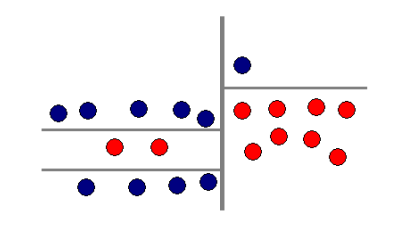
\includegraphics[scale=1.]{figures/feature_imp.png}
	\caption{ К вопросу о важности признака по частоте его выбора. Признак по оси $ x $ выбирается только один раз, а признак по оси $ y $ выбирается три раза, но очевидно, что первый признак лучше справляется с задачей }\label{fig:feature_imp}
\end{figure}

{\color{red}Нельзя отбрасывать признаки по порогу.}

Перестановочная важность признаков и важность признаков по Шепли обладают свойством \emph{согласованности} (если модель изменить так, что она более существенно начинает зависеть от какого-то признака, то его важность не убывает).

Подход вычисления \textbf{\itshape перестановочной важности признаков} (Permutation Feature Importance):
\begin{itemize}
	\item (+) не меняет распределение по конкретному признаку (так как рассматриваемый признак просто перемешивается),
	
	\item (+) не требует обучать модель заново -- обученную модель тестируют на \emph{\color{red}отложенной} выборке с \emph{\color{red}испорченным} признаком; то есть исходный набор данных разбивается на обучение и тест, модель обучается на обучающем поднаборе данных, на тестовом поднаборе мы вычисляем качество модели без модификации признаков, затем перетасовываем какой-то признак тестового поднабора и вычисляем качество на тестовом поднаборе с испорченным признаком, а затем делаем вывод о том на сколько качество изменилось (на сколько признак важен); Модель для вычисления важности признаков обучается на обучающем поднаборе данных, а \emph{важность признаков} вычисляется на \emph{\color{red}отложенной выборке}, включая различные схемы валидации; то есть можно было бы разбить исходный набор данных на $ k $ фолдов: обучаемся на $ k - 1 $ фолдах, вычисляем качество на \emph{валидационном} поднаборе данных без модификации признаков, затем применяем ту же самую модель (обученную на обучающем поднаборе данных первого разбиения) к валиадционному поднабору, но с уже перетасованным $ i $-ым признаком; и так поступаем для всех признаков $ f $ каждого фолда; теперь можно усреднить результаты по фолдам; в итоге мы получим $ f $ усредненных по фолдам важностей признаков,
	
	\item (+) можно применять на любых алгоритмах,
	
	\item (+) самый надежный метод,
	
	\item (+) в бутсрепе можно использовать OOB-контроль (строить дерево и на зкземплярах, не попавших в дерево, вычислять перестрановочную важность),
	
	\item (-) очень медленный.
\end{itemize}

\remark{
Вместо метрик качества для вычисления перестановочной важности можно использовать что-то другое. Например, долю верно классифицирующих деревьев
}

Идея перестановочной важности признаков: признак важный, если его перетасовка снижает качество. Можно вычислять перестановочную важность признаков на \emph{обучающем поднаборе данных} (вроде как бы можно, но лучше использовать отложенную выборку PFI-holdout), на \emph{отложенном контроле} (тестовый поднабор данных PFI-holdout, \pic{fig:PFI-holdout}) и на любой схеме \emph{валидации} (надежнее использовать валидацию). 

\begin{figure}[h]
	\centering
	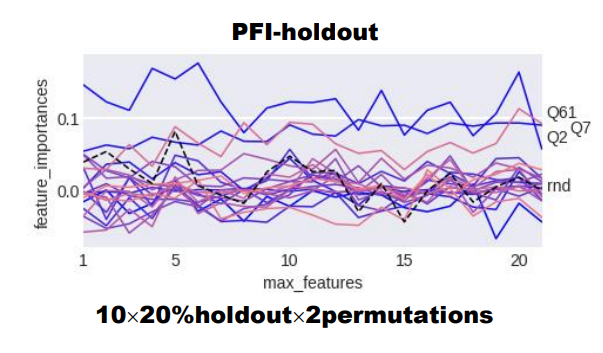
\includegraphics[scale=1.]{figures/PFI-holdout.png}
	\caption{ Перестановочная важность признаков, вычисленная на отложенной выборке }\label{fig:PFI-holdout}
\end{figure}

Перестановочная важность скоррелиррованных признаков может размазываться между ними.

Можно удалять признаки (Drop-column importance), но тогда каждый раз нужно будет заново обучать модель. Однако при этом результат более однозначный. Используется редко!

Если два признак коррелируют друг с другом, то перестановка одного из них не будет значимо сказываться на эффективности модели, потому что она может извлечь требуемую информацию из второго коррелирующего признака. Одним из способов работы с мультиколлинеарными признаками является иерархическая кластеризация на базе ранговых корреляций Спирмена, выбор порога отсечения и сохранение одного признака из каждого кластера.

\remark{
Важности признаков, полученные с помощью \texttt{feature\_importances\_} (важность по неоднородности), встроенного в алгоритмы построения ансамблей деревьев -- это НЕ важности признаков для решения задачи, а лишь для настройки конкретной модели. Этот подход не обладает свойством согласованности!!!}

В разделе 4.2.2 Relation to impurity-based importance in trees документации sklearn говорится, что impurity-based importance (\emph{важность признаков по неоднородности}; еще называют Gini importance) сильно смещена и отдает предпочтение \underline{высококардинальным} признакам (обычно вещественным) по сравнению с низкокардинальными признаками, такими как бинарные или категориальные признаки с небольшим числом категорий. Кроме того, важность по неоднородности годится только для деревьев и их ансамблей.

\textbf{\emph{Важность по Шепли}} $ i $-ого признака вычисляется следующим образом
\begin{align*}
	\varphi_i = \sum_{S \subseteq \{1, 2, \ldots, n\} \setminus \{i\}} \dfrac{ | S |! (n - |S| - 1)! }{ n! } \big( f(S \cup \{i\}) - f(S) \big),
\end{align*}
где $ f(S) $ -- ответ модели, обученной на подмножестве $ S $ множества $ n $ признаков (на конкретном объекте -- вся формула записывается для конкретного объекта).

Вычисление требует переобучения модели на всевозможных подмножествах признаков, поэтому на практике применяются приближения формулы, например, с помощью метода Монте-Карло.

Замечания по методам оценки важности признаков:
\begin{itemize}
	\item \underline{\itshape нет идеального алгоритма оценки важности признаков} (для любого можно подобрать пример, когда он плохо работает),
	
	\item если много похожих признаков (например, сильно коррелированных), то важность может <<делиться между ними>>, поэтому не рекомендуется отбрасывать признаки по порогу важности,
	
	\item есть старая рекомендация (впрочем, без теоретического обоснования): модель для решения задачи и оценки важности должны основываться на разных парадигмах (например, оценивать важность с помощью случайного леса и потом настраивать его же на важных признаках не рекомендуется). {\color{blue}То есть не рекомендуется оценивать важность и решать ML-задачу одним и тем же алгоритмом!!!}
\end{itemize}

Советы Дьяконова:
\begin{itemize}
	\item можно выбрать некоторое подмножество признаков и потом то добавить $ k $ признаков, то отнять $ l $,
	
	\item оценивать важность не обязательно с помощью лучшей модели (то есть не нужно строить супермодель для того, чтобы оценить важность признаков!)
	
	\item перестановочная важность самая естественная (но есть нюансы: коррелированность признаков, стабильность оценки и т.п.),
	
	\item есть и другие подходы и удобные библиотеки (SHAP, например).
\end{itemize}

\section{Приемы работы с библиотекой Polars}

\subsection{Уствновка}

Установить библиотеку Polars \url{https://www.pola.rs/} можно с помощью мендежера пакетов \texttt{pip}
\begin{lstlisting}[
style = ironpython,
numbers = none
]
pip install polars
\end{lstlisting}

С библиотекой Polars удобнее работать, использую оболочку \texttt{ptpython}.

\subsection{Вводные замечания}

Polars поддерживает режимы \emph{жадных} (eager)\footnote{В этом режиме работа с данными выглядит как в pandas} и \emph{отложенных} (lazy) вычислений.

Пример
\begin{lstlisting}[
style = ironpython,
numbers = none	
]
import polars as pl

df = pl.read_csv("https://j.mp/iriscsv")
print(
	df.filter(pl.col("sepal_length") > 5)
	.groupby("species")
	.agg(pl.all().sum())
)
\end{lstlisting}

Или в <<отложенном>> режиме
\begin{lstlisting}[
style = ironpython,
numbers = none
]
import polars as pl

print(
	pl.read_csv("https://j.mp/iriscsv")
	.lazy()  # набор данных сразу не загружается!
	.filter(pl.col("sepal_length") > 5)
	.groupby("species")
	.agg(pl.all().sum())
	.collect()
)
\end{lstlisting}

На Pandas этот запрос выглядел бы так
\begin{lstlisting}[
style = ironpython,
numbers = none
]
import numpy as np
import pandas as pd

df = pd.read_csv("https://j.mp/iriscsv")
df.loc[df.loc[:, "sepal_length"] > 5].groupby("species").agg(np.sum)
\end{lstlisting}

Если набор данных храниться \underline{\itshape локально}, то можно воспользоваться семейством функций \texttt{scan\_**}
\begin{lstlisting}[
style = ironpython,
numbers = none
]
pl.scan_csv("./iris.csv").\
    select(["sepal_width", "petal_width"]).\
    filter(pl.col("sepal_width") > 3.5).\
    collect()
\end{lstlisting}

Lazy API создает план выполнения запроса. Никакой шаг пайплайна не выполняется пока мы явно попросим Polars выполнить запрос (с помощью \verb*|LazyFrame.collect()| или \verb*|LazyFrame.fetch()|). Этот прием дает возможность Polars проанализировать весь запрос и выбрать наиболее подходящий по контексту алгоритм вычислений.


Чтобы перейти от жадного режима к ленивому достаточно просто начать запрос с \verb*|.lazy()|, а закончить \verb*|.collect()|.

\subsection{Polars-выражения}

Метод \texttt{filter} отбирает строки, а метод \texttt{select} -- столбцы.

Polars поддерживает очень мощную концепцию выражений. Рассмотрим несколько примеров
\begin{lstlisting}[
style = ironpython,
numbers = none,
]
out = df.select([
    pl.col("name").n_unique().alias("unique_names_1"),
    pl.col("name").unique().count().alias("unique_names_2")
])
\end{lstlisting}

Можно вызывать различные агрегаторы на объекте солбца
\begin{lstlisting}[
style = ironpython,
numbers = none
]
df.select(pl.col("name").std())
df.select(pl.col("name").max())
\end{lstlisting}

Можно выбирать столбцы по регулярному выражению
\begin{lstlisting}[
style = ironpython,
numbers = none
]
df.select(r"^Type\s{1}\d{1}$")  # выбирет столбцы 'Type 1', 'Type 2' etc.
\end{lstlisting}

Можно использовать фильтры и условия. В фильтр передается булева маска
\begin{lstlisting}[
style = ironpython,
numbers = none
]
df.select([
    pl.col("species").filter(
        pl.col("species").str.contains(r".*osa$")
    ).count() # count() -- это метод объекта столбца
])  # 50
\end{lstlisting}

На Pandas этот запрос выглядел бы так
\begin{lstlisting}[
style = ironpython,
numbers = none
]
df.loc[
    df.loc[:, "species"].str.contains(r".*osa$")  # вернет булеву маску
]["species"].count()  # 50

# или так
df.loc[
    df.loc[:, "species"].str.contains(r".*osa$")  # вернет булеву маску
].shape[0]  # 50
\end{lstlisting}

Можно использовать конструкцию \emph{when} $ \rightarrow $ \emph{then} $ \rightarrow $ \emph{otherwise}
\begin{lstlisting}[
style = ironpython,
numbers = none	
]
df.select([
    pl.when(pl.col("petal_length") > 3)
    .then(100)
    .otherwise(pl.col("sepal_width") * 10) * pl.col("sepal_length").sum()
])
\end{lstlisting}

На Pandas запрос выглядел бы так
\begin{lstlisting}[
style = ironpython,
numbers = none
]
np.where(
    df.loc[:, "petal_length"] > 3,
    100,
    df.loc[:, "sepal_width"] * 10
) * df.loc[:, "sepal_length"].sum()
\end{lstlisting}

Еще пример
\begin{lstlisting}[
style = ironpython,
numbers = none
]
# Polars
(
    df
    .lazy()
    .groupby("species")
    .agg(pl.all().sum())
    .select(["species", "petal_length"])
    .collect()
)

# Pandas
(
    df
    .groupby("species")
    .agg(np.sum)[["species", "petal_lenth"]]
)
\end{lstlisting}

Пример группировки с последующим построением агрегата
\begin{lstlisting}[
style = ironpython,
numbers = none
]
df.groupby("species").agg([
    pl.col("sepal_width").mean(),
    pl.col("petal_length").max(),
]).sort("species")
\end{lstlisting}

На Pandas
\begin{lstlisting}[
style = ironpython,
numbers = none
]
df.groupby("species").agg({
    "sepal_width": np.mean,
    "petal_length": np.max,
}).sort_index()
\end{lstlisting}

Если нужны склеить поэлементно строковые столбцы, то лучше воспользоваться функцией \verb*|pl.concat_str([...])|, а не fold-выражением, так как из-за материализации промежуточных столбцов у fold-выражений будет квадратичная временная сложность
\begin{lstlisting}[
style = ironpython,
numbers = none
]
df.select([
    pl.concat_str(["a", "b"])  # "a" и "b" это имена столбцов
])
\end{lstlisting}

Polars-выражения нельзя использовать везде. Вот допустимые \emph{контексты}:
\begin{itemize}
	\item \verb*|df.select([...])|
	
	\item \verb*|df.groupby(...).agg([...])|
	
	\item \verb*|df.with_columns([...])|
\end{itemize}

Даже в тех случаях, когда мы явно работаем в <<жадном>> режиме, на самом деле используется режим отложенных вычислений
\begin{lstlisting}[
style = ironpython,
numbers = none
]
df.groupby("foo").agg([pl.col("bar").sum()])
# на самом деле
(df.lazy().groupby("foo").agg([pl.col("bar").sum()])).collect()
\end{lstlisting}

Добавить столбец (или несколько столбцов) можно так
\begin{lstlisting}[
style = ironpython,
numbers = none
]
df.with_columns([
    (pl.col("sepal_length").sum() + pl.col("petal_width")).alias("new_col_1"),
    pl.col("sepal_length").mean().alias("new_col_2")
])
\end{lstlisting}

Создать производный столбец с кастомной функцией можно так
\begin{lstlisting}[
style = ironpython,
numbers = none
]
df.with_columns([
    pl.col("Speed").map(f=lambda elem: elem ** 2).alias("SquaredSpeed")
])
\end{lstlisting}

Если псевдоним не задать, то метод \verb*|with_columns| перезапишет существующий столбец \texttt{"Speed"}. Но \verb*|with_columns| возвращает новый объект.

\remark{
\color{red}
Пользовательские Python-функции убивают распараллеливание!
}

Можно также фильтровать группы. Пусть требуется вычислить среднее по группе, но не для всех элементов группы. Для ясности можно использовать Python-функции. Они ничего не стоят, потому как применяются только в Polars-выражении, а на шаге выполнения запроса
\begin{lstlisting}[
style = ironpython,
numbers = none	
]
from datetime import date

import polars as pl

from .dataset import dataset


def compute_age() -> pl.Expr:
	return date(2021, 1, 1).year - pl.col("birthday").dt.year()


# здесь мы вычисляем временную дельту для столбца 'birthday',
# а фильтруем по ассоциированным строкам столбца 'gender'
def avg_birthday(gender: str) -> pl.Expr:
	return compute_age().filter(pl.col("gender") == gender).mean().alias(f"avg {gender} birthday")


q = (
	dataset.lazy()
	.groupby(["state"])
	.agg(
		[
			avg_birthday("M"),
			avg_birthday("F"),
			(pl.col("gender") == "M").sum().alias("# male"),
			(pl.col("gender") == "F").sum().alias("# female"),
		]
	)
	.limit(5)
)

df = q.collect()
\end{lstlisting}

С помощью метода \texttt{filter} мы отбираем строки в столбце \texttt{'gender'}, а затем по оставшимся строкам столбца \texttt{'gender'} вычисляем среднее и связываем результат с псевдонимом.

Еще вместо группировки можно использовать фильтр по одному столбцу и агрегацию по другому столбцу
\begin{lstlisting}[
style = ironpython,
numbers = none	
]
df.select([
    pl.col("sepal_width").filter(pl.col("species") == "setosa").mean()
])  # 3.418
\end{lstlisting}

На Pandas было бы так
\begin{lstlisting}[
style = ironpython,
numbers = none	
]
df.loc[df.loc[:, "species"] == "setosa", "sepal_width"].mean()
\end{lstlisting}

\subsection{Оконные функции}

Оконную функцию из обычной можно сделать, вызвав метод $ \verb*|.over()| $.

Пример
\begin{lstlisting}[
style = ironpython,
numbers = none	
]
df.select(["Type 1", "Type 2", "Attack", "Defense"]).select([
	"Type 1",
	"Type 2",
	pl.col("Attack").mean().over("Type 1").alias("avg_attack_by_type"),
	pl.col("Defense").mean().over(["Type 1", "Type 2"]).alias("avg_defense_by_type_comb"),
])
\end{lstlisting}

Добавить столбец \texttt{"WinCumsum"} с кумулятивной суммой по группе
\begin{lstlisting}[
style = ironpython,
numbers = none	
]
df.select([
    "Type 1",
    "Speed",
    pl.col("Speed").cumsum().over("Type 1").alias("WinCumsum"),
]).sort("Type 1")
\end{lstlisting}

Еще пример оконной функции. NB: столбцы, которые используются в \verb*|.over([...])| должны быть отсортированы
\begin{lstlisting}[
style = ironpython,
numbers = none	
]
df.sort("Type 1").select([
    pl.col("Type 1").head(3).list().over("Type 1").flatten(),
    pl.col("Name").sort_by("Attack").head(3).list().over("Type 1").flatten().alias("fastest/group"),
    pl.col("Name").sort_by(pl.col("Speed")).head(3).list().over("Type 1").flatten().alias("strongest/group"),
])
\end{lstlisting}

\subsection{Универсальные NumPy-функции}

Polars поддерживает универсальные numpy-функции \verb*|ufuncs| \url{https://numpy.org/doc/stable/reference/ufuncs.html#available-ufuncs}.

Пример
\begin{lstlisting}[
style = ironpython,
numbers = none
]
df.select([
    np.log(pl.all()).suffix("_log")  # pl.all() -- применяется ко всем столбцам
])
\end{lstlisting}

\subsection{Примеры}

Столбцы можно выбирать по регулярному выражению
\begin{lstlisting}[
style = ironpython,
numbers = none
]
df.select([
    pl.col(r"^Type\s{1}\d{1}$")  # Polars-выражение
])

# или так
df.select(r"^Type\s{1}\d{1}$")

df.select([
    pl.col(r"^Sp.*$").sum()
])
\end{lstlisting}

С помощью конструкции \texttt{pl.all()} можно выбирать все столбцы в таблице (работает также как \verb*|*| в SQL-запросах)
\begin{lstlisting}[
style = ironpython,
numbers = none
]
df.select([
    pl.all().reverse().suffix("_rev")  # выбрать все столбцы в обратном порядке
])

df.select([
    pl.all().sum().suffix("_sum")  # найти сумму по всем столбцам
])
\end{lstlisting}

Polars-выражения можно связывать с переменными
\begin{lstlisting}[
style = ironpython,
numbers = none
]
mask = pl.col("Type 1").str.contains(r"^Gr.*$")

df.select([
    mask.sum(),  # найти количество элементов, удовлетворяющих шаблону
])

df.select([
    pl.col("Speed").filter(mask).sum(),
])
\end{lstlisting}

Пример с when-then-otherwise
\begin{lstlisting}[
style = ironpython,
numbers = none	
]
df.select([
    "Type 1",
    pl.when(pl.col("Type 1") == "Grass")
    .then(pl.col("Type 2").str.to_uppercase())
    .otherwise(pl.col("Name").str.to_lowercase())
])
\end{lstlisting}

Пример с оконными функциями
\begin{lstlisting}[
style = ironpython,
numbers = none
]
df.select([
    "fruits",
    "cars",
    "B",
    pl.col("B").sum().over("fruits").alias("B_sum_by_fruits"),
    pl.col("B").sum().over("cars").alias("B_sum_by_cars"),
])
\end{lstlisting}

Сумма вычисляется по группе и транслируется на все элементы группы.

Приклеить столбец справа можно с помощью метода \texttt{hstack}
\begin{lstlisting}[
style = ironpython,
numbers = none
]
df: pl.DataFrame
df.hstack([
    pl.Series("new_col", np.random.randint(10, 100, size=df.height))
])
\end{lstlisting}

Вставить столбец в произвольную позицию можно так
\begin{lstlisting}[
style = ironpython,
numbers = none
]
# insert_at_idx изменяет объект на месте
df.insert_at_idx(0, pl.Series("new_col", np.random.randn(df.heigth)))
\end{lstlisting}

\subsection{Работа с временными рядами}

Pandas-конструкцию \verb*|ts.resample(...).agg(...)| силами Polars можно реализовать так
\begin{lstlisting}[
style = ironpython,
numbers = none
]
ts.groupby_dynamic(
    "time_stamp",
    every="4h",
    closed="left",
).agg([
    pl.col("value").count().alias("value_cnt"),
    pl.col("value").mean().suffix("_mean"),
])
\end{lstlisting}


\section{Приемы работы с библиотекой Catboost}

Онлайн документация пакета \url{https://catboost.ai/en/docs/concepts/python-reference_catboostregressor}.

\subsection{Установка CatBoost}

Установить пакет можно с помощью менеджера \texttt{conda} (или с помощью \texttt{pip})
\begin{lstlisting}[
style = bash,
numbers = none
]
$ conda config --show channels
# если канала conda-forge нет в списке, то следует его добавить 
$ conda config --add channels conda-forge
$ conda install catboost
$ pip install catboost
\end{lstlisting}

\subsection{Ключевые особенности пакета}

\subsection{Параметры}

\remark{
Помимо \texttt{iterations} и \texttt{learning\_rate} у CatBoost 5 важнейших гиперпараметров: \texttt{max\_depth}, \texttt{l2\_leaf\_reg}, \texttt{border\_count}, \texttt{random\_strength} и \texttt{bagging\_temperature}
}

Применительно к \texttt{random\_strength} замечено, что часто значение, близкое к 0 (примерно, 0.15), дает лучшее качество. Если переменных много, можно попробовать настраивать \texttt{rsm}.

В случае дисбаланса классов будет полезным настраивать
\begin{itemize}
	\item либо гиперпараметр \texttt{auto\_class\_weights},
	
	\item либо гиперпараметры \texttt{class\_weights} и \texttt{scale\_pos\_weight}
\end{itemize}
при этом не нужно настраивать эти параметры одновременно.

Можно сначала при \emph{небольшом} числе итераций найти оптимальные значения гиперпараметров, \emph{меньше} всего зависящие от количества итераций (речь прежде всего идет об \texttt{auto\_class\_weights}, \texttt{max\_depth}; при этом \texttt{learning\_rate} и \texttt{rsm} зависят от количества итераций, поэтому нам для небольшого количества итераций придется увеличить темп обучения, а варьирование \texttt{rsm} сделать минимальным). Затем можно построить модель с найденными оптимальными значениями гиперпараметров  \texttt{auto\_class\_weights}, \texttt{max\_depth} и \texttt{rsm}, но уже с большим количеством деревьев, при этом, разумеется помня о двух вещах:
\begin{itemize}
	\item при большом количестве итераций нужно уменьшить темп обучения,
	
	\item выбирая меньшее значение \texttt{rsm}, нужно задавать больше итераций.
\end{itemize}

Ознакомится с описанием параметров можно здесь \url{https://catboost.ai/en/docs/references/training-parameters/}

Общие параметры:
\begin{itemize}
	\item \verb|loss_function| (objective) -- функция потерь, которая используется на шаге обучения модели.
	
	\item \texttt{iterations} -- максимальное число деревьев в ансамбле,
	
	\item \verb*|learning_rate| -- темп обучения,
	
	\item \verb*|l2_leaf_reg| -- коэффициент при члене $ L_2 $-регуляризации,
	
	\item \verb*|bagging_temperature| -- задает настройки Байесовского бутстрапа
\end{itemize}



\subsection{Классификатор CatBoostClassfier}

Класс \texttt{CatBoostClassifier}

\begin{lstlisting}[
style = ironpython,
numbers = none	
]
class CatBoostClassifier(
		iterations=None,
		learning_rate=None,
		depth=None,
		l2_leaf_reg=None,
		model_size_reg=None,
		rsm=None,
		loss_function=None,
		border_count=None,
		feature_border_type=None,
		per_float_feature_quantization=None,                         
		input_borders=None,
		output_borders=None,
		fold_permutation_block=None,
		od_pval=None,
		od_wait=None,
		od_type=None,
		nan_mode=None,
		counter_calc_method=None,
		leaf_estimation_iterations=None,
		leaf_estimation_method=None,
		thread_count=None,
		random_seed=None,
		use_best_model=None,
		verbose=None,
		logging_level=None,
		metric_period=None,
		ctr_leaf_count_limit=None,
		store_all_simple_ctr=None,
		max_ctr_complexity=None,
		has_time=None,
		allow_const_label=None,
		classes_count=None,
		class_weights=None,
		one_hot_max_size=None,
		random_strength=None,
		name=None,
		ignored_features=None,
		train_dir=None,
		custom_loss=None,
		custom_metric=None,
		eval_metric=None,
		bagging_temperature=None,
		save_snapshot=None,
		snapshot_file=None,
		snapshot_interval=None,
		fold_len_multiplier=None,
		used_ram_limit=None,
		gpu_ram_part=None,
		allow_writing_files=None,
		final_ctr_computation_mode=None,
		approx_on_full_history=None,
		boosting_type=None,
		simple_ctr=None,
		combinations_ctr=None,
		per_feature_ctr=None,
		task_type=None,
		device_config=None,
		devices=None,
		bootstrap_type=None,
		subsample=None,
		sampling_unit=None,
		dev_score_calc_obj_block_size=None,
		max_depth=None,
		n_estimators=None,
		num_boost_round=None,
		num_trees=None,
		colsample_bylevel=None,
		random_state=None,
		reg_lambda=None,
		objective=None,
		eta=None,
		max_bin=None,
		scale_pos_weight=None,
		gpu_cat_features_storage=None,
		data_partition=None
		metadata=None,
		early_stopping_rounds=None,
		cat_features=None,
		grow_policy=None,
		min_data_in_leaf=None,
		min_child_samples=None,
		max_leaves=None,
		num_leaves=None,
		score_function=None,
		leaf_estimation_backtracking=None,
		ctr_history_unit=None,
		monotone_constraints=None,
		feature_weights=None,
		penalties_coefficient=None,
		first_feature_use_penalties=None,
		model_shrink_rate=None,
		model_shrink_mode=None,
		langevin=None,
		diffusion_temperature=None,
		posterior_sampling=None,
		boost_from_average=None,
		text_features=None,
		tokenizers=None,
		dictionaries=None,
		feature_calcers=None,
		text_processing=None
)
\end{lstlisting}

LogLoss применяется для задач бинарной классификации (когда целевей вектор содиржит только два уникальных значения или когда параметр \verb|target_border is not None|).

MultiClass используется в задачах мультиклассовой классификации (когда целевой вектор содержит более 2 уникальных значений или параметр \verb|border_count is None|)

\subsection{Регрессор CatBoostRegressor}

Помимо \texttt{iterations} и \texttt{learning\_rate} у CatBoost 5 важнейших гиперпараметров:
\begin{itemize}
	\item \texttt{max\_depth}: мак,
	
	\item \texttt{l2\_leaf\_reg},
	
	\item \texttt{border\_count},
	
	\item \texttt{random\_strength},
	
	\item \texttt{bagging\_temperature}.
\end{itemize}

\subsection{Функции потерь и метрики качества}

\subsubsection{Для классификации}

Для мультиклассификации \url{https://catboost.ai/en/docs/concepts/loss-functions-multiclassification}

\emph{Функции потерь}
\begin{itemize}
	\item LogLoss
\begin{align*}
	- \dfrac{ \sum\limits_{i=1}^N w_i \big( c_i \log p_i + (1 - c_i) \log (1 - p_i) \big) }{ \sum\limits_{i=1}^{N} w_i },
\end{align*}

    \item CrossEntropy
\begin{align*}
	- \dfrac{ \sum\limits_{i=1}^N w_i \big( t_i \log p_i + (1 - t_i) \log (1 - p_i) \big) }{ \sum\limits_{i=1}^{N} w_i },
\end{align*}
\end{itemize}

\emph{Метрики качества}
\begin{itemize}
	\item Precision (точность),
	
	\item Recall (полнота),
	
	\item F1 (гармоническое среднее),
	
	\item BalancedAccuracy
\begin{align*}
	\dfrac{1}{2} \Big( \dfrac{TP}{T} + \dfrac{TN}{N} \Big),
\end{align*}

    \item BalancedErrorRate
\begin{align*}
	\dfrac{1}{2} \Big( \dfrac{FP}{TN + FP} + \dfrac{FN}{FN + TP} \Big),
\end{align*}

    \item AUC,
    
    \item BrierScore,
    
    \item HingeLoss,
    
    \item HammingLoss
\begin{align*}
	\dfrac{ \sum\limits_{i=1}^{N} w_i [[p_i > 0.5] == t_i] }{ \sum\limits_{i=1}^{N} w_i},
\end{align*}

    \item Kappa
\begin{align*}
	1 - \dfrac{1 - Accuracy}{1 - RAccuracy},\\
	RAccuracy = \dfrac{ (TN + FP) (TN + FN) + (FN + TP)(FP + TP) }{ \Big( \sum\limits_{i=1}^{N} w_i \Big)^2 }
\end{align*}

    \item LogLikelihoodOfPrediction.
\end{itemize}

\subsubsection{Для регрессии}

\emph{Метрики качества, которые могут играть роль функции потерь}

\begin{itemize}
	\item MultiRMSE (в случае мультирегрессии)
\begin{align*}
	\Biggl( \dfrac{ \sum\limits_{i=1}^N \sum\limits_{d=1}^{dim} (a_{i,d} - t_{i,d})^2 w_i }{ \sum\limits_{i=1}^N w_i } \Biggr)^{1/2}
\end{align*}
	
	\item MAE
\begin{align*}
	\dfrac{ \sum\limits_{i=1}^{N} w_i | a_i - t_i |}{ \sum\limits_{i=1}^{N} w_i },
\end{align*}

    \item MAPE
\begin{align*}
	\dfrac{ \sum\limits_{i=1}^{N} w_i \dfrac{ | a_i - t_i | }{ \max (1, | t_i |) } }{ \sum\limits_{i=1}^N w_i }
\end{align*}

    \item Poisson
\begin{align*}
	\dfrac{ \sum\limits_{i=1}^N w_i (e^{ a_i } - a_i t_i) }{ \sum\limits_{i=1}^N w_i },
\end{align*}

   \item Quantile (большие значения $ \alpha $ сильнее штрафуют за заниженные прогнозы)
\begin{align*}
	\dfrac{ \sum\limits_{i=1}^N \Big( \alpha - 1[t_i \leqslant a_i] \Big) (t_i - a_i) w_i}{ \sum\limits_{i=1}^N w_i },
\end{align*}

    \item RMSE
\begin{align*}
	\Bigg( \dfrac{ \sum\limits_{i=1}^N (a_i - t_i)^2 w_i }{ \sum\limits_{i=1}^N w_i } \Bigg)^{1/2}
\end{align*}

    \item LogLinQuantile,
    
    \item Lq
\begin{align*}
	\dfrac{\sum\limits_{i=1}^N | a_i - t_i |^q w_i}{ \sum\limits_{i=1}^N w_i }
\end{align*}

    \item Huber
\begin{align*}
	L(t, a) = \sum_{i=0}^N l(t_i, a_i) \cdot w_i,\quad l(t, a) = 
	\begin{cases}
		\dfrac{1}{2} (t - a)^2, &| t - a | \leqslant \delta,\\
		\delta | t - a | - \dfrac{1}{2} \delta^2, &| t - a | > \delta.
	\end{cases}
\end{align*}

\item Excpectile
\begin{align*}
	\dfrac{ \sum\limits_{i=1}^N | \alpha - 1[t_i \leqslant a_i] | (t_i - a_i)^2 w_i }{ \sum\limits_{i=1}^N w_i }
\end{align*}

\item Tweedie
\begin{align*}
	\dfrac{ \sum\limits_{i=1}^N \Big( \dfrac{e^{a_i (2 - \lambda)}}{2 - \lambda} - t_i \dfrac{ e^{a_i ( 1 - \lambda)} }{ 1 - \lambda } \Big) w_i }{ \sum\limits_{i=1}^N w_i },
\end{align*}
где $ \lambda $ -- значение параметра дисперсии мощности,
\end{itemize}

\emph{Метрики качества}

\begin{itemize}
	\item SMAPE
\begin{align*}
	\dfrac{ 100 \sum\limits_{i=1}^N \dfrac{ w_i | a_i - t_i | }{ (|t_i| + |a_i|)/2 } }{ \sum\limits_{i=1}^N w_i }
\end{align*}

    \item R2 (коэффициент детерминации)
\begin{align*}
	1 - \dfrac{ \sum\limits_{i=1}^N w_i (a_i - t_i)^2 }{ \sum\limits_{i=1}^N w_i (\bar{t} - t_i)^2 }.
\end{align*}

    \item MSLE (среднеквадратическая логарифмическая ошибка)
\begin{align*}
	\dfrac{ \sum\limits_{i=1}^N w_i \big( \ln (1 + t_i) - \ln (1 + a_i) \big)^2 }{ \sum\limits_{i=1}^N w_i }
\end{align*}

    \item MedianAbsoluteError
\begin{align*}
	median(|t_1 - a_1|, \ldots, |t_N - a_N|)
\end{align*}
\end{itemize}


\section{Приемы работы с решателем SCIP}

Полезный ресурс \url{https://www.gams.com/37/docs/S_SCIP.html#INDEX_SCIP_2d__21_solver}

Пример конфигурационного файла настроек решателя (если файл \texttt{scip.set} лежит в директории, из-под которой запускается сеанс SCIP, то этот файл будет использован для настройки сеанса)
\begin{lstlisting}[
title = {\sffamily scip.set},
style = bash,
numbers = none
]
propagating/probing/maxprerounds = 0
separating/maxrounds = 0
separating/maxroundsroot = 0
\end{lstlisting}

\subsection{Общие сведения}

Задачи линейного программирования в частично-целочисленной линейной постановке относятся к классу NP-трудных. Это означает, что мы знаем ни одного алгоритма, способного решать задачи такого типа за время, которое масштабируется как полином от длины входа (от размера задачи).

Выбор правила выбора переменной играет фундаментальную роль в разработке алгоритмов и оказывает значительное влияние на время решения.

\subsection{Emphasis Settings}

SCIP поддреживает следующие настройки выразительности (emphasis):
\begin{itemize}
	\item \texttt{set emphasis easycip}: для простых проблем,
	
	\item \texttt{set emphasis feasibility}: для поиска осуществимого решения,
	
	\item \texttt{set emphasis hardlp}: для решения LP-трудных задач,
	
	\item \texttt{set emphasis optimality}: для доказательства оптимальности,
	
	\item \texttt{set emphasis numerics}: для повышения численной устойчивости,
	
	\item \texttt{set heuristics emphasis aggressive}: для агрессивного применения первичных эверистк,
	
	\item \texttt{set heuristics emphasis fast}: будут использованы только быстрые эвристики,
	
	\item \texttt{set heuristics emphasis off}: отключает все первичные эвристики,
	
	\item \texttt{set presolving emphasis aggressive}: для агрессивной предобработки,
	
	\item \texttt{set presolving emphasis fast}: для будут использованы только быстрые шаги предобработки,
	
	\item \texttt{set presolving emphasis off}: отключает предобработку,
	
	\item \texttt{set separaing emphasis aggressive}: для агрессивного использования разделителей,
	
	\item \texttt{set separating emphasis fast}: будут использованы только быстрые разделители,
	
	\item \texttt{set separating emphasis off}: отключает все разделители.
\end{itemize}

\subsection{Проблемы <<using pseudo solution instead>>}

\url{https://www.scipopt.org/doc/html/CONS.php}

Обратный вызов \texttt{CONSENFOPS} аналогичен обратному вызову \texttt{CONSENFOLP}, но имеет дело с пседорешениями вместо LP-решений. Если LP-задача не была решена в текущей подзадаче (либо потому, что пользователь не захотел ее решать, либо потому, что возникли трудности в процессе решения LP-задачи), LP-решение не доступно. В этом случае используется пседо-решение. В этом решении переменные устанавливаются на локальную границу, которая является наилучшей по отношению к целевой функции. О пседо-решении можно думать как о релаксированном решении со всеми ограничениями за исключением удаляемых границ.


\section{Приемы работы с библиотеками Gym и Ecole}

\subsection{Gym}

Функция окружения (environment) \texttt{step} возвращает четыре значения:
\begin{itemize}
	\item \verb|observation| (object):  это объект, специфичный для окружающей среды и представляющий результат наблюдения за этой средой (например, состояние доски в настольной игре),
	
	\item \verb|reward| (float): вознаграждение, полученное за предыдущее действие. Масштаб варьируется в зависимости от среды, но цель всегда в том, чтобы сделать суммарное вознаграждение как можно больше,
	
	\item \verb|done| (boolean): флаг завершения эпизода. Многие (но не все) задачи разделены на четко определенные эпизоды, и \texttt{done = True} указывает на то, что эпизод завершился (например, мы потеряли последнюю жизнь в игре),
	
	\item \verb|info| (dict): диагонстическая информация, полезная для отладки.
\end{itemize}

Это просто реализация классического цикла <<агент -- среда>>. На каждом шаге агент совершает то или иное действие и среда возвращает наблюдения (observation) и вознаграждение (reward).

Процесс запускается вызовом функции \verb|reset()|, которая возвращает первое приближение \texttt{observation}.  
\begin{lstlisting}[
style=ironpython,
numbers=none
]
import gym
env = gym.make('CartPole-v0')
for i_episode in range(20):
    observation = env.reset()
    for t in range(100):
        env.render()
        print(observation)
        action = env.action_space.sample()
        observation, reward, done, info = env.step(action)
        if done:
            print("Episode finished after {} timesteps".format(t+1))
            break
env.close()
\end{lstlisting}

В этом примере мы отбирали случайные действия из пространства действий среды. Каждая среда поставляется с атрибутами \verb|action_space| и \verb|observation_space|. Эти атрибуты имеют тип \verb|Space| и описывают формат допустимых действий и наблюдений
\begin{lstlisting}[
style=ironpython,
numbers=none
]
import gym

env = gym.make("CartPole-v0")
print(env.action_space)  # Discrete(2)

print(env.observation_space)  # Box([-4.8000002e+00 -3.4028235e+38 -4.1887903e-01 -3.4028235e+38], [4.8000002e+00 3.4028235e+38 4.1887903e-01 3.4028235e+38], (4,), float32)
\end{lstlisting}

Пространство \texttt{Descrete} описывает фиксированный диапазон неотрицательных чисел, так что в данном случае допустимыми действиями будет 0 или 1. Пространство \texttt{Box} представляет $ n $-мерный ящик, так что в данном случае допустимыми наблюдениями будут 4-мерные массивы.

\subsection{Ecole}

Полезный ресурс о специальных приемах работы с задачами линейного программирования в частично-целочисленного постановке \url{https://www.gams.com/37/docs/UG_LanguageFeatures.html?search=sos1}

Полезный ресурс по математической оптимизации \url{https://scipbook.readthedocs.io/en/latest/}

\subsubsection{Общие сведения}

Обучение с подкреплением это уникальная парадигма машинного обучения в силу особенностей формулировки цели на базе системы вознаграждения.

Гипотеза о вознаграждении: цель агента -- максимизировать накполенную сумму вознаграждений.

На каждом шаге агент выбирает действие, базируясь на политике $ \pi(s) $. Эта политика может быть детерминированной и в этом случае она становится просто отображением состояний на действия.

Однако, как правило политика стохастическая, что означает, что каждому состоянию назначается функция распределения вероятностей по пространству действий
\begin{align*}
	\pi (a | s) := \mathbb{P} (A_t = a | S_t = s).
\end{align*}

Цель агента состоит в том, чтобы максимизировать накопленное вознаграждение
\begin{align*}
	G_t := \sum_{k=t+1}^T \gamma^{k-t-1} R_k,
\end{align*}
где $ \gamma \in [0, 1] $ -- коэффициент дисконтирования.

Таким образом, $ \gamma $ определяет компромисс между немедленным и будущим вознаграждением. Это формализует идею о том, что действия влияют на последующие состояния и, следовательно, имеют последствия, выходящие за рамки мгновенного вознаграждения. 

Линейное программирование в частично-целочисленной постановке (Mixed Integer Linear Program, MILP) это проблема линейного программирования, когда и ограничения и целевая функция линейные, а некоторые переменные могут принимать целочисленные значения.

Задачи MILP относятсу к классу NP-трудных. На практике это означает, что на текущий момент не известно алгоритмов, способных решить задачу за полиномиальное время.

\emph{Секущие плоскости} были одним из первых предложенных решений для борьбы с MILP. Ключевая идея состоит в том, чтобы начать с естественной  линейной релаксации допустимых множеств и постепенно ужесточать эту релаксацию, отбрасывая области , которые не являются частью выпуклой оболочки. Этот подход сводит MILP к последовательному решению задач линейного программирования.



\subsubsection{Observations}

Класс \texttt{ecole.observation.NodeBipartiteObs}: двудольный граф наблюдений для узлов branch-and-bound дерева. Оптимизационная задача представляется в виде гетерогенного двудольного графа. Между переменной и ограничением будет существовать ребро, если переменная присутствует в ограничении с ненулевым коэффициентом.

Метод \texttt{reset()} в Ecole принимает в качестве аргумента экземпляр проблемы. 

\subsubsection{Анализ примера работы связки Ecole+GNN}

В рассматриваемом примере проводится анализ упрощенной реализации решения Gasse et al. (2019). Мы будем использовать генератор экземпляров, предоставленный Ecole
\begin{lstlisting}[
style = ironpython,
numbers = none
]
instances = ecole.instance.SetCoverGenerator(n_rows=500, n_cols=1000, density=0.05)
\end{lstlisting}

В схеме <<исследование, а затем сильное ветвление>>, чтобы разнообразить состояния, в которых мы собираем примеры сильного ветвления, мы в основном следуем за слабым, но дешевым экспертом (pseudocost branching) и лишь изредка вызываем сильного эксперта (strong branching). Это также гарантирует, что выборки будут ближе к тому, чтобы быть независимыми и одинаково распределенными.

Это можеть быть реализовано в Ecole путем создания пользовательской функции наблюдения (observation function), которая будет случайным образом вычислять и возвращать оценки псевдооценки (дешево) или оценки сильного ветвления (дорого)
\begin{lstlisting}[
style = ironpython,
numbers = none	
]
class ExploreThenStrongBranch:
	"""
	This custom observation function class will randomly return either strong branching scores (expensive expert)
	or pseudocost scores (weak expert for exploration) when called at every node.
	"""

	def __init__(self, expert_probability):
		self.expert_probability = expert_probability
		self.pseudocosts_function = ecole.observation.Pseudocosts()
		self.strong_branching_function = ecole.observation.StrongBranchingScores()

	def before_reset(self, model):
		"""
		This function will be called at initialization of the environment (before dynamics are reset).
		"""
		self.pseudocosts_function.before_reset(model)
		self.strong_branching_function.before_reset(model)

	def extract(self, model, done):
		"""
		Should we return strong branching or pseudocost scores at time node?
		"""
		probabilities = [1 - self.expert_probability, self.expert_probability]
		expert_chosen = bool(np.random.choice(np.arange(2), p=probabilities))
		if expert_chosen:
			return (self.strong_branching_function.extract(model, done), True)
		else:
			return (self.pseudocosts_function.extract(model, done), False)
\end{lstlisting}

\begin{lstlisting}[
style = ironpython,
numbers = none
]
# We can pass custom SCIP parameters easily
scip_parameters = {
	"separating/maxrounds": 0,
	"presolving/maxrestarts": 0,
	"limits/time": 3600,
}

# Note how we can tuple observation functions to return complex state information
env = ecole.environment.Branching(
	observation_function=(
		ExploreThenStrongBranch(expert_probability=0.05),
		ecole.observation.NodeBipartite(),
	),
	scip_params=scip_parameters,
)

# This will seed the environment for reproducibility
env.seed(0)
\end{lstlisting}

\begin{lstlisting}[
style = ironpython,
numbers = none
]
episode_counter, sample_counter = 0, 0
Path("samples/").mkdir(exist_ok=True)

# We will solve problems (run episodes) until we have saved enough samples
while sample_counter < DATA_MAX_SAMPLES:
	episode_counter += 1

	observation, action_set, _, done, _ = env.reset(next(instances))
	while not done:
		(scores, scores_are_expert), node_observation = observation
		action = action_set[scores[action_set].argmax()]

		# Only save samples if they are coming from the expert (strong branching)
		if scores_are_expert and (sample_counter < DATA_MAX_SAMPLES):
			sample_counter += 1
			data = [node_observation, action, action_set, scores]
			filename = f"samples/sample_{sample_counter}.pkl"

			with gzip.open(filename, "wb") as f:
				pickle.dump(data, f)

		observation, action_set, _, done, _ = env.step(action)

	print(f"Episode {episode_counter}, {sample_counter} samples collected so far")
\end{lstlisting}

Обучение графовой нейронной сети
\begin{lstlisting}[
style = ironpython,
numbers = none
]
DEVICE = torch.device("cuda" if torch.cuda.is_available() else "cpu")
\end{lstlisting}

\begin{lstlisting}[
style = ironpython,
numbers = none
]
class BipartiteNodeData(torch_geometric.data.Data):
	"""
	This class encode a node bipartite graph observation as returned by the `ecole.observation.NodeBipartite`
	observation function in a format understood by the pytorch geometric data handlers.
	"""

	def __init__(
		self,
		constraint_features,
		edge_indices,
		edge_features,
		variable_features,
		candidates,
		nb_candidates,
		candidate_choice,
		candidate_scores,
	):
		super().__init__()
		self.constraint_features = constraint_features
		self.edge_index = edge_indices
		self.edge_attr = edge_features
		self.variable_features = variable_features
		self.candidates = candidates
		self.nb_candidates = nb_candidates
		self.candidate_choices = candidate_choice
		self.candidate_scores = candidate_scores

	def __inc__(self, key, value, store, *args, **kwargs):
		"""
		We overload the pytorch geometric method that tells how to increment indices when concatenating graphs
		for those entries (edge index, candidates) for which this is not obvious.
		"""
		if key == "edge_index":
			return torch.tensor(
				[[self.constraint_features.size(0)], [self.variable_features.size(0)]]
			)
		elif key == "candidates":
			return self.variable_features.size(0)
		else:
			return super().__inc__(key, value, *args, **kwargs)


class GraphDataset(torch_geometric.data.Dataset):
	"""
	This class encodes a collection of graphs, as well as a method to load such graphs from the disk.
	It can be used in turn by the data loaders provided by pytorch geometric.
	"""

	def __init__(self, sample_files):
		super().__init__(root=None, transform=None, pre_transform=None)
		self.sample_files = sample_files

	def len(self):
		return len(self.sample_files)

	def get(self, index):
		"""
		This method loads a node bipartite graph observation as saved on the disk during data collection.
		"""
		with gzip.open(self.sample_files[index], "rb") as f:
			sample = pickle.load(f)

		sample_observation, sample_action, sample_action_set, sample_scores = sample

		constraint_features = sample_observation.row_features
		edge_indices = sample_observation.edge_features.indices.astype(np.int32)
		edge_features = np.expand_dims(sample_observation.edge_features.values, axis=-1)
		variable_features = sample_observation.column_features

		# We note on which variables we were allowed to branch, the scores as well as the choice
		# taken by strong branching (relative to the candidates)
		candidates = np.array(sample_action_set, dtype=np.int32)
		candidate_scores = np.array([sample_scores[j] for j in candidates])
		candidate_choice = np.where(candidates == sample_action)[0][0]

		graph = BipartiteNodeData(
			torch.FloatTensor(constraint_features),
			torch.LongTensor(edge_indices),
			torch.FloatTensor(edge_features),
			torch.FloatTensor(variable_features),
			torch.LongTensor(candidates),
			len(candidates),
			torch.LongTensor([candidate_choice]),
			torch.FloatTensor(candidate_scores)
		)

		# We must tell pytorch geometric how many nodes there are, for indexing purposes
		graph.num_nodes = constraint_features.shape[0] + variable_features.shape[0]

		return graph
\end{lstlisting}

Архитектура нейронной сети
\begin{lstlisting}[
style = ironpython,
numbers = none
]
class GNNPolicy(torch.nn.Module):
	def __init__(self):
		super().__init__()
		emb_size = 64
		cons_nfeats = 5
		edge_nfeats = 1
		var_nfeats = 19

	# CONSTRAINT EMBEDDING
	self.cons_embedding = torch.nn.Sequential(
		torch.nn.LayerNorm(cons_nfeats),
		torch.nn.Linear(cons_nfeats, emb_size),
		torch.nn.ReLU(),
		torch.nn.Linear(emb_size, emb_size),
		torch.nn.ReLU(),
	)

	# EDGE EMBEDDING
	self.edge_embedding = torch.nn.Sequential(
		torch.nn.LayerNorm(edge_nfeats),
	)

	# VARIABLE EMBEDDING
	self.var_embedding = torch.nn.Sequential(
		torch.nn.LayerNorm(var_nfeats),
		torch.nn.Linear(var_nfeats, emb_size),
		torch.nn.ReLU(),
		torch.nn.Linear(emb_size, emb_size),
		torch.nn.ReLU(),
	)

	self.conv_v_to_c = BipartiteGraphConvolution()
	self.conv_c_to_v = BipartiteGraphConvolution()

	self.output_module = torch.nn.Sequential(
		torch.nn.Linear(emb_size, emb_size),
		torch.nn.ReLU(),
		torch.nn.Linear(emb_size, 1, bias=False),
	)

	def forward(
		self, constraint_features, edge_indices, edge_features, variable_features
	):
		reversed_edge_indices = torch.stack([edge_indices[1], edge_indices[0]], dim=0)

		# First step: linear embedding layers to a common dimension (64)
		constraint_features = self.cons_embedding(constraint_features)
		edge_features = self.edge_embedding(edge_features)
		variable_features = self.var_embedding(variable_features)

	# Two half convolutions
	constraint_features = self.conv_v_to_c(
		variable_features, reversed_edge_indices, edge_features, constraint_features
	)
	variable_features = self.conv_c_to_v(
		constraint_features, edge_indices, edge_features, variable_features
	)

	# A final MLP on the variable features
	output = self.output_module(variable_features).squeeze(-1)
	return output


class BipartiteGraphConvolution(torch_geometric.nn.MessagePassing):
	"""
	The bipartite graph convolution is already provided by pytorch geometric and we merely need
	to provide the exact form of the messages being passed.
	"""

	def __init__(self):
		super().__init__("add")
		emb_size = 64

		self.feature_module_left = torch.nn.Sequential(
			torch.nn.Linear(emb_size, emb_size)
		)
		self.feature_module_edge = torch.nn.Sequential(
			torch.nn.Linear(1, emb_size, bias=False)
		)
		self.feature_module_right = torch.nn.Sequential(
			torch.nn.Linear(emb_size, emb_size, bias=False)
		)
		self.feature_module_final = torch.nn.Sequential(
			torch.nn.LayerNorm(emb_size),
			torch.nn.ReLU(),
			torch.nn.Linear(emb_size, emb_size),
		)
		
		self.post_conv_module = torch.nn.Sequential(torch.nn.LayerNorm(emb_size))
		
		# output_layers
		self.output_module = torch.nn.Sequential(
			torch.nn.Linear(2 * emb_size, emb_size),
			torch.nn.ReLU(),
			torch.nn.Linear(emb_size, emb_size),
		)

	def forward(self, left_features, edge_indices, edge_features, right_features):
		"""
		This method sends the messages, computed in the message method.
		"""
		output = self.propagate(
			edge_indices,
			size=(left_features.shape[0], right_features.shape[0]),
			node_features=(left_features, right_features),
			edge_features=edge_features,
		)
		return self.output_module(
			torch.cat([self.post_conv_module(output), right_features], dim=-1)
		)

	def message(self, node_features_i, node_features_j, edge_features):
		output = self.feature_module_final(
			self.feature_module_left(node_features_i)
			+ self.feature_module_edge(edge_features)
			+ self.feature_module_right(node_features_j)
		)
		return output


policy = GNNPolicy().to(DEVICE)
\end{lstlisting}




\section{Нейронные сети}

Теорема об универсальной аппроксимации (Hornik, 1991)

\emph{Любую} непрерывную функцию можно с любой точностью приблизить нейросетью глубины 2 с \emph{сигмоидной функцией активации} на скрытом слое и \emph{линейной функцией} на выходном слое.

Нейросеть глубины два с фиксированной функцией активации в первом слое и линейной функцией активации во втором слое может равномерно аппроксимировать (может быть при увеличении числа нейронов на первом слое) любую непрерывную функцию на компактном множестве тогда и только тогда, когда функция активации \emph{неполиномиальная}.

Что плохого в сигмоиде:
\begin{itemize}
	\item <<убивает>> градиенты,
	
	\item выходы не отцентрированы (легко устранить с помощьд $ \tanh $),
	
	\item вычисление экспоненты все-таки накладно
\end{itemize}

\remark{
Обратное распространение = SGD + дифференцирование сложных функций (\pic{fig:backprop})
}

\begin{figure}[h]
	\centering
	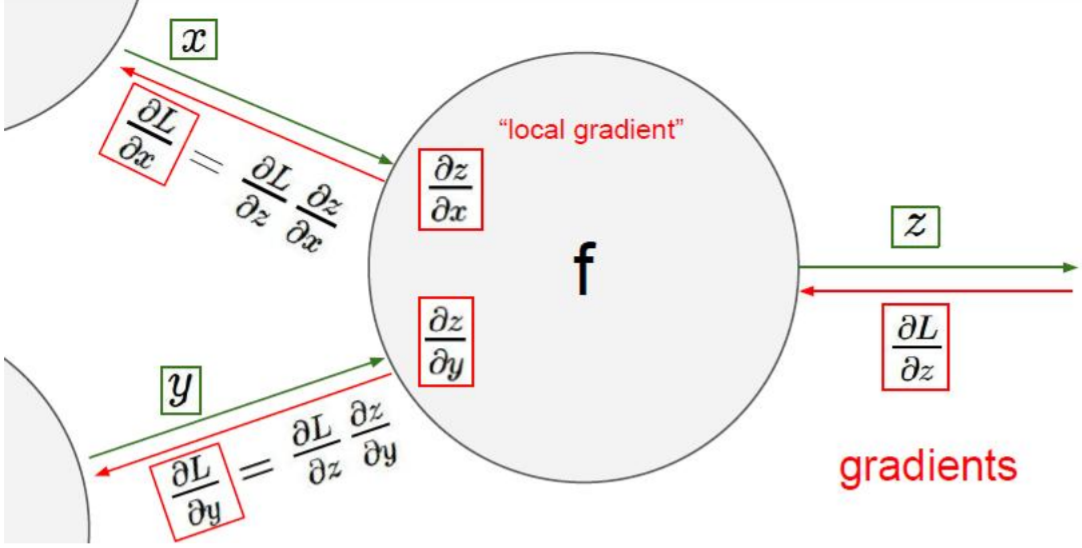
\includegraphics[scale=0.5]{figures/backprop.png}
	\caption{ Прямое распространение сигнала и обратное распространение градиента }\label{fig:backprop}
\end{figure}

\section{Приемы работы с библиотекой \texttt{marshmallow}}

\emph{Сериализация} ({dumping}) -- это процедура преобразования объекта или дерева объектов в какой-либо формат, по которому потом эти объекты можно восстановить. Используется, например, для сохранения состояния программы (то есть некоторых ее объектов) между запусками. Или для передачи данных по сети. 

Основная идея заключается в том, что сериализованный формат -- это \emph{последовательность байт} или \emph{строка}.

Обратная процедура называется \emph{десериализацией} (loading).

Например, для сериализации с помощью модуля \texttt{json} можно поступить так
\begin{lstlisting}[
style = ironpython,
numbers = none
]
import json

d = {"key1": 10, "key2": 20}

# для преобрзвания дерева объектов в последовательность байтов
with open("./make_json.json", mode="w") as f:
    json.dump(d, fp=f) # словарь -> файл

# для преобразования дерева объектов в строку
json.dumps(d)  # вернет строку '{"key1": 10, "key2": 20}'
\end{lstlisting}

Объявим класс данных
\begin{lstlisting}[
style = ironpython,
numbers = none
]
from marshmallow import Schema, fields, validate, ValidationError

# объявляем структуру данных
class PersonSchema(Schema):
    name = fields.String(
        required=True,
        validate=validate.Regexp("^Le.*$")
    )
    age = fields.Integer(
        required=True,
        validate=validate.Range(min=18, max=45)
    )
    job = fields.String(
        required=False,
        validate=validate.Length(min=3)
    )
    email = fields.Email(required=False)
    sex = fields.String(load_default="male")  # это значение по умолчанию будет использоваться на шаге десериализации

# проверка на согласованность 
person_leor = PersonSchema().load({
    "name": "Leor",
    "age": 35,
    "job": "Data Scientist",
    "email": "leor.finkelberg@yandex.ru",
})

type(person_leor)  # dict
\end{lstlisting}

Если переданный словарь отвечает стуктуре данных, то метод \verb*|load()| класса \verb*|PersonSchema| этот же словарь и вернет. Но если хотя бы одно значение нарушает требования поля, то будет возбуждено исключение \verb*|ValidationError|. Поэтому строки вызова метода \verb*|load| следует оборачивать с помощью \verb*|try-except|
\begin{lstlisting}[
style = ironpython,
numbers = none	
]
schema = PersonSchema()
leor = {"name": "Leor", ...}
try:
    # метод load прогоняет словарь через структуру данных
    # и если все хорошо, то этот же словарь и возвращает
    person_leor: dict = PersonSchema().load(leor)
except ValidationError as err:
    print(err.messages, err.valid_data)
\end{lstlisting}


\section{Борьба с переобучением в нейронных сетях}

\subsection{Нормировка}

Пусть даны признаки $ X = \{X_1, \ldots, X_m\} $.

Тогда

\emph{среднее признака}
\begin{align*}
	\mu = \dfrac{1}{m} \sum_{i=1}^m X_i,
\end{align*}

\emph{дисперсия признака}
\begin{align*}
	\sigma^2 = \dfrac{1}{m} \sum_{i=1}^m (X_i - \mu)^2
\end{align*}

\emph{нормировка}
\begin{align*}
	X = \dfrac{X - \mu}{\sqrt{\sigma^2}}
\end{align*}

\subsection{Инициализация весов}

Инициализация весов:
\begin{itemize}
	\item нарушить симметричность (чтобы нейроны были разные),
	
	\item недопустить насыщение нейрона (почти всегда близок к 0 или 1),
	
	\item ключевая идея -- входы на все слои должны иметь одинаковую дисперсию (для избегания <<насыщения>> нейронов).
\end{itemize}

Инициализация по Ксавье [Glorot \& Bengio, 2010]
\begin{align*}
	w_{ij}^{(k)} \sim U \Bigg[ - \sqrt{ \dfrac{ 6 }{ n_{in}^{(k)} + n_{out}^{(k)}} }, + \sqrt{ \dfrac{ 6 }{ n_{in}^{(k)} + n_{out}^{(k)}} } \, \Bigg].
\end{align*}

Дисперсия весов
\begin{align*}
	D[ w_{ij}^{(k)} ] = \dfrac{ 2 }{ n_{in}^{(k)} + n_{out}^{(k)} }.
\end{align*}

Формула выведена в предположении, что нет нелинейностей, т.е. $ z^{(k+1)} = f(W^{(k)} z^{(k)}) \equiv W^{(k)} z^{(k)} $.

Смотрим ошибку на отложенной выборке! Выбираем итерацию, на которой ошибка наименьшая (\pic{fig:lear_rate}).

\begin{figure}[h]
	\centering
	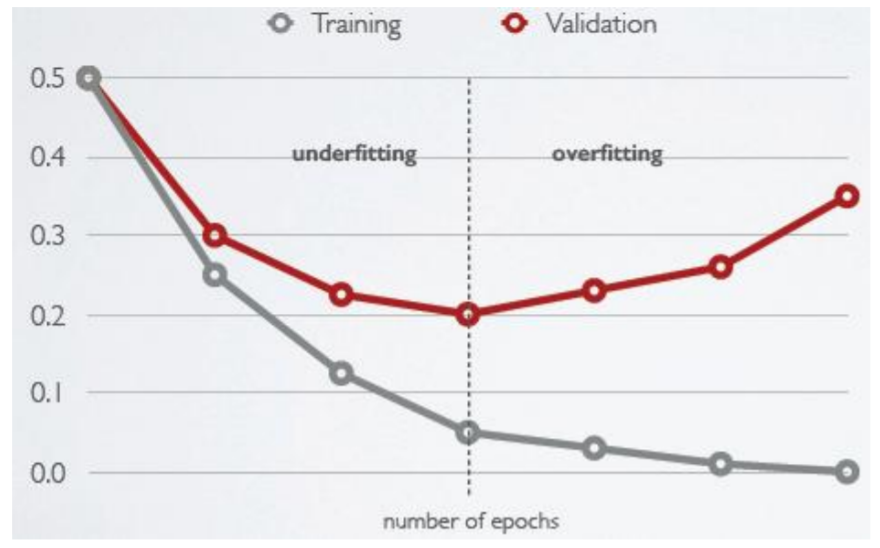
\includegraphics[scale=0.5]{figures/lear_rate.png}
	\caption{ Настройка темпа обучения }\label{fig:lear_rate}
\end{figure}

Увеличение размера пакета -- тот же эффект, что и уменьшение темпа обучения.

\subsection{Продвинутая оптимизация}

Стохастический градиент (надо случайно перемешивать данные перед каждой эпохой)
\begin{align*}
	w^{(t+1)} = w^{(t)} - \eta \, \nabla L^{(t)}(w^{(t)}).
\end{align*}

Стохастический градиент с моментом (Momentum)
\begin{align*}
	m^{(t+1)} = \rho \, m^{(t)} + \nabla L^{(t)}(w^{(t)}),\\
	w^{(t+1)} = w^{(t)} - \eta \, m^{(t+1)} = \underbrace{ w^{(t)} - \eta \, \nabla L^{(t)}(w^{(t)}) }_{\text{\itshape стохастический градиент}}+ \underbrace{- \eta \, \rho \, m^{(t)}}_{\text{\itshape добавление инерции}}.
\end{align*}

Метод Нестерова
\begin{align*}
	m^{(t+1)} = \rho \, m^{(t)} + \nabla L^{(t)} (w^{(t)} - \eta \, m^{(t)}),\\
	w^{(t+1)} = w^{(t)} - \eta \, m^{(t+1)} = w^{(t)} - \eta \, \nabla L^{(t)}(w^{(t)} + \underbrace{\color{blue} - \eta \, m^{(t)}}_{\text{\itshape\color{blue} смещение}}) + \underbrace{\color{blue} - \eta \, \rho \, m^{(t)} }_{\text{\itshape\color{blue} добавление инерции}}.
\end{align*}

\section{Графовые нейронные сети}

Полезные ресурсы Distill
\begin{itemize}
	\item \url{https://distill.pub/2021/understanding-gnns/},
	
	\item \url{https://distill.pub/2021/gnn-intro/}.
\end{itemize}


Графовые нейронные сети (GNN) вычисляют предаставления вершин в итеративном процессе, разные виды GNN по-разному, каждая итерация соответствует слою сети. Самая простая концепция такого вычисления -- неронное распространение (Neural Message Passing). Вообще, распространение сообщений довольно известный прием в анализе графов, заключается в том, что каждая вершина имеет некоторое состояние, которое за одну итерацию уточняется по следующей формуле
\begin{align*}
	h_v^{(k)} = \text{UPDATE}^{(k)} \Big( h_v^{(k-1)},  \text{AGG}^{(k)} (\{ h_u^{(k-1)} \}_{u \in N(v)}) \Big),
\end{align*}
где $ N(v) $ -- окрестной вершины $ v $, $ \text{AGG} $ -- функция аггрегации (по смыслу она собирает информацию о соседях, например, суммируя состояния), $ \text{UPDATE} $ -- функция обновления состояния вершины (с учетом собранной информации о сосдениях).

Единственное требование, которое накладывается на последние две функции -- дифференциируемость, чтобы использовать их в вычислительном графе и вычислять параметры сети методом обратного распространения.

\noindent\emph{Для графовых сверточных нейронных сетей}

\begin{align*}
	h_v^{(0)} = x_v, \ \forall v \in V,
\end{align*}
где $ h_v^{(0)} $ -- начальное представление узла $ v $, $ x_v $ -- оригинальные признаки узла $ v $.

И теперь для каждого шага $ k = 1, 2, \ldots, K $ [Distill]
\begin{align*}
	h_v^{(k)} = f^{(k)} \Big( W^{(k)} \cdot \dfrac{ \sum\limits_{ u \in N(v) } h_u^{(k-1)} }{ |N(v)| } + B^{(k)} \cdot h_v^{(k-1)}\Big), \ \forall v \in V,
\end{align*}
где $ h_v^{(k)} $ -- представление узла $ v $ на шаге $ k $, $ h_v^{(k-1)} $ -- представление узла $ v $ на шаге $ k - 1 $.

\remark{
Веса $ W^{(k)} $ и $ B^{(k)} $ разделяются между всеми узлами графа
}

Выражение справа от коэффициента $ W^{(k)} $ -- среднее представлений соседей вершины $ v $ на шаге $ k - 1 $.

Построить прогноз на каждом узле можно с помощью последнего вычисленного представления
\begin{align*}
	\hat{y}_v = \text{PREDICT}(h_v^{(K)}),
\end{align*}
где $ \text{PREDICT} $ -- как правило, другая нейронная сеть, обученная вместе с моделью GCN.

\remark{
GCN хорошо масштабируется, поскольку количество параметров в модели не привязано к размеру графа
}

Пример (\pic{fig:GCN}). Для вершины $ A $ на шаге 1 представление можно вычислить следующим образом, опросив соседей вершины
\begin{align*}
	h_A^{(1)} &= f\Big( W^{(1)} \times \dfrac{ h_E^{(0)} + h_F^{(0)} + h_G^{(0)} }{ 3 } + B^{(1)} \times h_A^{(0)} \Big) \\
	&= f(1 \times \dfrac{ 2 + (-2) + 0 }{ 3 } + 1 \times -4) \\
	&= f(0 + (-4)) \\
	&= f(-4) \\
	&= ReLU(-4) = 0.
\end{align*}

\begin{figure}[h]
	\centering
	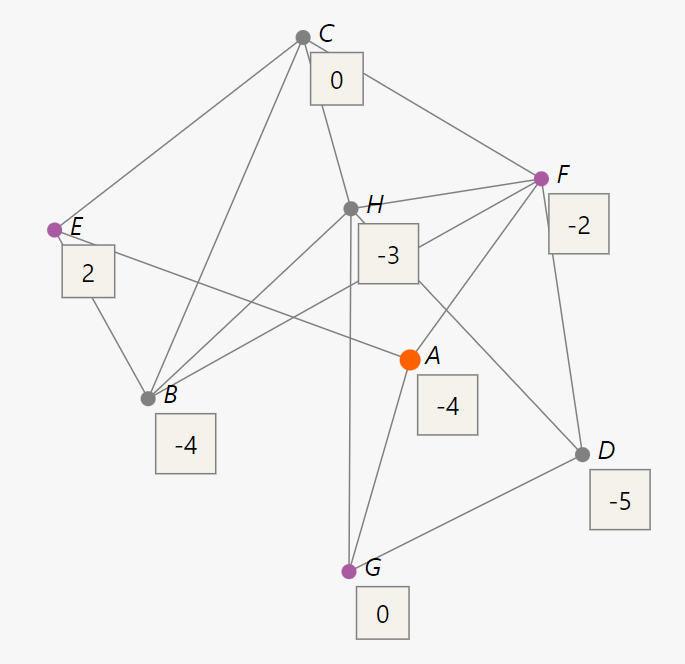
\includegraphics[scale=0.5]{figures/GCN.png}
	\caption{ Пример вычисления обновленного представления узла $ A $ на шаге 1 \\в графовой сверточной нейронной сети }\label{fig:GCN}
\end{figure}

На практике каждая описанная выше итерация обычно рассматривается как один <<слой нейронной сети>>. Этой идеологии придерживаются многие популярные библиотеки графовых нейронных сетей (PyTorch Geometic, StellarGraph), позволяющие создавать различные типы сверток графа в одной и той же модели.

Методы, которые мы рассматривали до сих пор, выполняют <<локальные>> свертки: признак каждого узла обновляется с использованием информации о признаках его локальных соседей. Однако можно построить и <<глобальную>> свертку.

После выбора произвольного порядка узлов мы можем собрать все признаки в вектор $ x \in \mathbb{R} $.

После нормализации $ x $ как $ \sum\limits_{i=1}^n x_i^2 = 1 $
\begin{align*}
	R_L(x) = \dfrac{ x^T Lx }{ x^T x} = \dfrac{ \sum_{(i,j) \in E} (x_i - x_j)^2 }{ \sum_i x_i^2 } = \sum_{ (i, j) \in E } (x_i - x_j)^2.
\end{align*} 

Множество собственных чисел лапласиана $ L $ называют \emph{спектром}. Спектральное разложение
\begin{align*}
	L = U \Lambda U^T, \ \Lambda = \text{diag}(\lambda_1, \ldots, \lambda_n), \ U = \{u_1 \ldots u_n\}, \ U^T U = I,
\end{align*}
где $ \Lambda $ -- диагональная матрица отсортированных собственных чисел, $ U $ -- обозначает матрицу собственных векторов, отсортированных по возрастанию собственных чисел.

Каждый вектор признаков $ x $ может быть представлен в виде линейной комбинации собственных векторов
\begin{align*}
	x = \sum_{i=1}^n \hat{x}_i u_i = U \hat{x},
\end{align*}
где $ \hat{x} $ -- это вектор коэффициентов $ [x_0, \ldots, x_n] $. Будем называть $ \hat{x} $ \emph{спектральным представлением} вектора признаков $ x $.

\remark{
Свертку в спектральной области графа можно рассматривать как обобщение свертки в частотной области изображений
}

Теория спектральных сверток математически обоснована, но есть несколько нюаносов:
\begin{itemize}
	\item Нам требуется вычислить матрицу собственных векторов $ U_m $. Для больших графов это неосуществимо,
	
	\item Даже если мы сможем вычислить $ U_m $, сами глобальные свертки неэффективны из-за повторяющегося умножения,
	
	\item Изученные фильтры специфичны для графов, поскольку они представлены в терминах спектрального разложения входного графа Лапласиана. Это означает, что они плохо переносятся на новые графы, которые имеют существенно иную структуру (и, следовательно, существенно разные собственные значения).
\end{itemize}

Хотя спекртальные свертки в значительной степени были вытеснены <<локальными>> свертками по рассмотренным выше причинам, все еще имеет смысл изучать идеи, лежащие в их основе.

Функции потерь для различных задач на графах:
\begin{itemize}
	\item Классификация узлов:
\begin{align*}
	\mathcal{L}(y_v, \hat{y}_v) = - \sum_c y_{vc} \log \hat{y}_{vc},
\end{align*}
где $ \hat{y}_{vc} $ -- предсказанная вероятность того что узел $ v $ принадлежит классу $ c $. GNNs адаптированы и для обучения на частично-размеченных данных, когда только некоторые узлы имеют разметку. В этом случае функцию потерь можно так
\begin{align*}
	\mathcal{L}_G = \dfrac{ \sum\limits_{ v \in \text{ Lab }(G) } \mathcal{L}(y_v, \hat{y}_v)}{ | \text{Lab}(G) | },
\end{align*}
где потери можно вычислить только на размеченных узлах $ \text{Lab}(G) $.

    \item Классификация графа: собрав информацию о представлении узлов графа, можно составить векторное представление графа. 
    
    \item Предсказание вероятности появления связи: опираясь на пары смежных и несмежных узлов, можно использовать их векторные представления в качестве входных данных для прогнозирования наличия / отсутствия связи
\begin{align*}
	\mathcal{L}(y_v, y_u, e_{vu}) = - e_{vu} \log (p_{vu}) - (1 - e_{vu}) \log(1 - p_{vu}),\\
	p_{vu} = \sigma (y_v^T y_u),
\end{align*}
где $ \sigma $ -- логистический сигмоид, и $ e_{vu} = 1 $, если между узлами $ v $ и $ u $ есть связь, и $ e_{vu} = 0 $ в противном случае.

    \item Кластеризация узлов: простая кластеризация представлений узлов.
\end{itemize}

Основная проблема при использовании описываемого нейронного распространения, т.н. \emph{чрезмерное сглаживание} (over-smoothing): после нескольких итераций пересчета состояний вершин представления соседних вершин становятся похожими, поскольку у них похожие окрестности. Для борьбы с этим делают
\begin{itemize}
	\item меньше слоев агрегации и больше для <<обработки признаков>>,
	
	\item прокидывание слоев или конкатенацию состояний с предыдущих слоев,
	
	\item используют архитектуры, в которых есть эффект памяти,
	
	\item приемы с номировками,
	
	\item используют аугментацию, например, DropEdge,
	
	\item используют noise regularization.
\end{itemize}

Сводка по графовым нейронным сетям
\begin{itemize}
	\item На вход сети подается граф, каждая вершина которого имеет признаковое описание. Это описание можно считать начальным состоянием вершины,
	
	\item Могут быть слои, которые независимо модифицируют представления (для каждой вершины его представление пропускается через небольшую нейронку),
	
	\item Могут быть слои, которые модифицируют представления всех вершин, учитывая представления вершин-соседей,
	
	\item Могут быть слои, упрощающие граф (например, уменьшающие число вершин),
	
	\item Могут быть слои, получающие представление графа (вектор фиксированной длины) по текущему графу с представлениями вершин.
\end{itemize}



\section{Отбор признаков с библиотекой BoostARoota}

BoostARoota \url{https://github.com/chasedehan/BoostARoota} -- алгоритм отобора признаков на базе экстримального градиентного бустинга в реализации XGBoost. Алгоритм требует гораздо меньших затрат времени на выполнение. Перед применением необходимо выполнить дамми-кодирование, поскольку базовая модель работает только с количественными признаками.

Отбор признаков выполняется на обучающем поднаборе данных, поэтому предполагается, что массив меток и массив признаков \emph{обучающие}, а для проверки качества модели отбора признаков есть независимая, \emph{тестовая} выборка. Кроме того, если необходимо выбрать оптимальные значения гиперпараметров модели отбора признаков (например, значения гиперпараметров \texttt{cutoff}, \texttt{iters} и \texttt{delta}), то понадобиться еще \emph{проверочная} {выборка}.

\section{Классический и байесовский бутстреп}

Бутстреп является универсальным инструментом для оценки статистической точности. 

Байесовский бутстреп это байевоский аналог классического бутстрапа. Вместо моделирования распределения выборки для статистики, оценивающей параметр, байесовский бутстреп моделирует \emph{апостериорное распределение параметра}. 

Основная идея состоит в том, чтобы случайным образом извлекать наборы данных с \underline{возвращением} из обучающих данных так, чтобы каждая выборка имела тот же размер, что и исходное обучающее множество.Это делается $ B $ раз (скажем, $ B = 100 $), создавая $ B $ множеств бутстрепа. Затем мы заново аппроксимируем модель для каждого из множест бутстрепа и исследуем поведение аппроксимаций на $ B $ выборках.

По выборке бутстрепа мы можем оценить любой аспект распределения $ S(\mathbf{Z}) $ (это любая величина, вычисленная по данным $ \mathbf{Z} $), например, его дисперсию
\begin{align*}
	\widehat{ Var }[ S(\mathbf{Z}) ] = \dfrac{1}{B - 1} \sum_{b=1}^{B} \Big( S(\mathbf{Z}^{*b})  - \bar{S}^* \Big)^2, \quad \bar{S}^{*} = \sum_b S( \mathbf{Z}^{*b} ) / B.
\end{align*}

\section{HDI}

Highest Density Interval (HDI) -- интервал высокой плотности -- показывает какие точки распределения наиболее достоверны/правдоподобны и охватывают большую часть распределения. Каждая точка внутри интервала имеет более высокую \emph{достоверность}, чем любая точка вне интервала.

\section{Площадь по ROC-кривой}

Построение ROC-кривой происходит следующим образом (\pic{fig:roc_auc0}):
\begin{enumerate}
	\item  Сначала сортируем все наблюдения по убыванию спрогнозированной вероятности положительного класса,
	
	\item Берем единичный квадрат на координатной плоскости. Значения оси абсцисс будут значениями 1 - специфичности (цена деления оси задается значением 1/neg), а значения оси ординат будут значениями чувствительности (цена деления оси задается значением 1/pos). При этом pos — это количество наблюдений положительного класса, а neg — количество наблюдений отрицательного класса,
	
	\item Задаем точку c координатами (0, 0) и для каждого отсортированного наблюдения x:
	\begin{itemize}
		\item если x принадлежит положительному классу, двигаемся на 1/pos вверх,
		
		\item если x принадлежит отрицательному классу, двигаемся на 1/neg вправо.
	\end{itemize}
\end{enumerate}

Значение вероятности положительного класса, при котором ROC-кривая находится на минимальном расстоянии от верхнего левого угла -- точки с координатами (0, 1), дает наибольшую правильность классификации. В данному случае (\pic{fig:roc_auc0-1}) будет 0.72.

\begin{figure}[h]
	\centering
	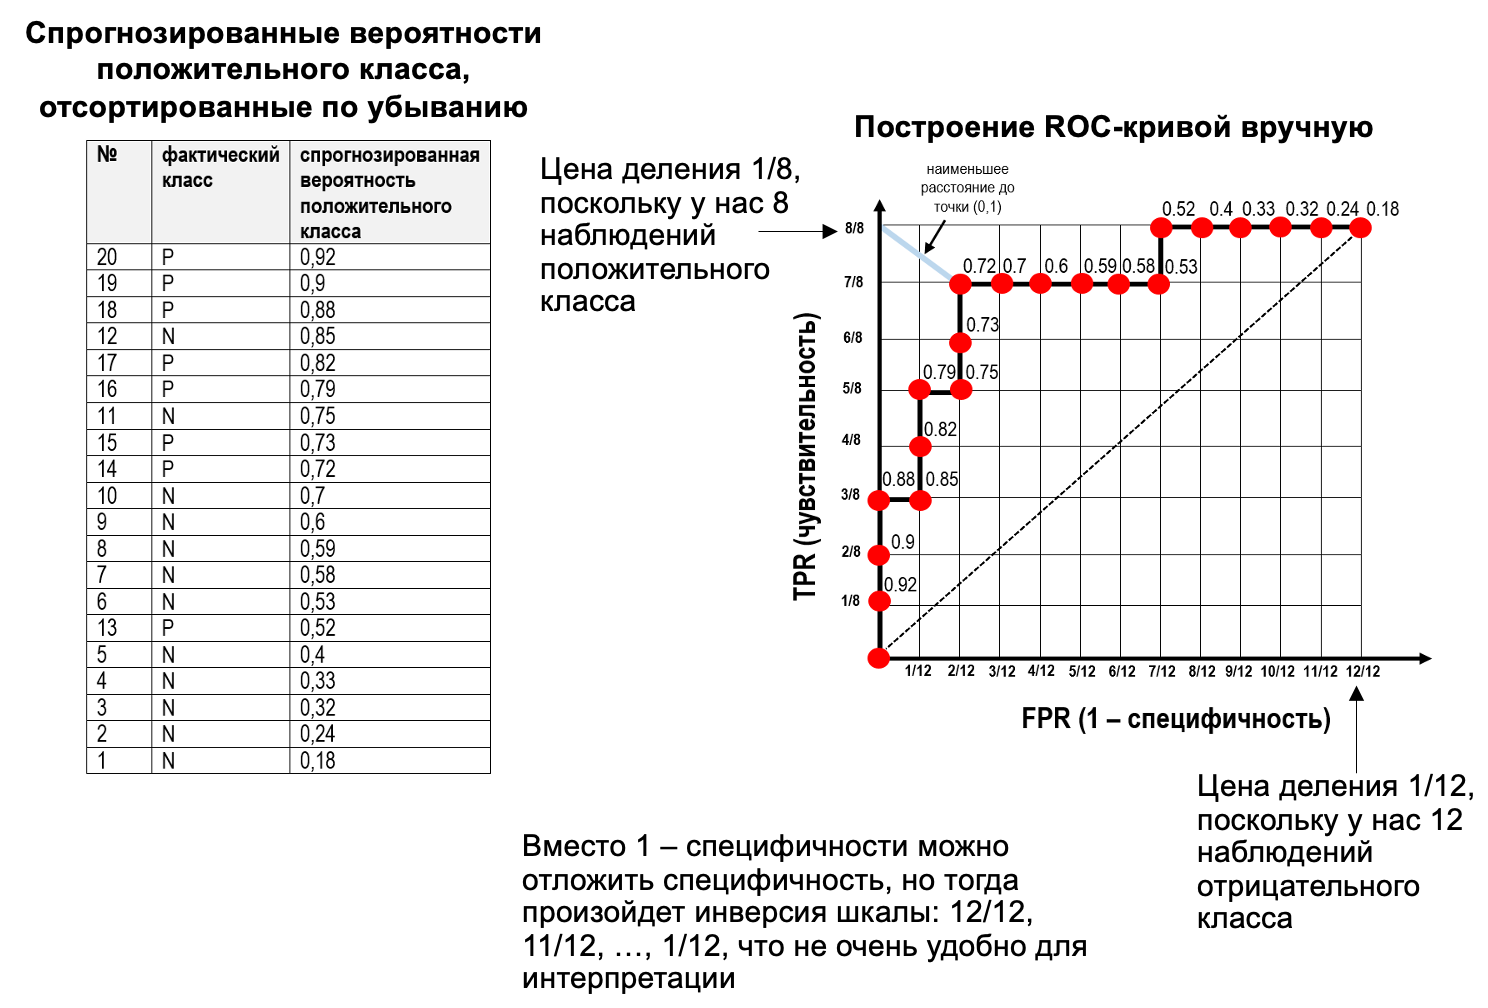
\includegraphics[scale=0.3]{figures/roc_auc0.png}
	\caption{ Построение ROC-кривой }\label{fig:roc_auc0}
\end{figure}

\begin{figure}[h]
	\centering
	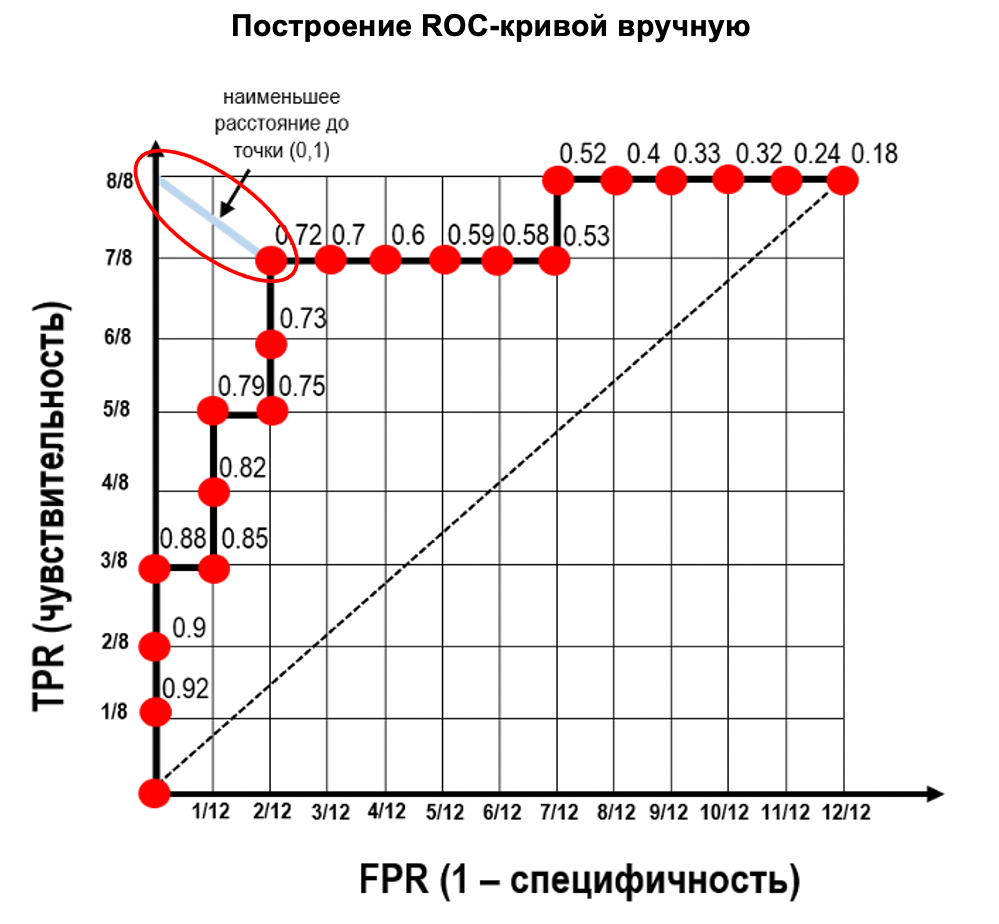
\includegraphics[scale=0.3]{figures/roc_auc0-1.png}
	\caption{ ROC-кривая. Порог отсечения 0.72 }\label{fig:roc_auc0-1}
\end{figure}

Площадь под ROC-кривой (ROC-AUC) можно интерпретировать как вероятность события, состоящего в том, что классификатор присвоит более высокий ранг (например, вероятность) случайно выбранному экземпляру положительного класса, чем случайно выбранному экземпляру отрицательного класса (если не рассматривать вариант равенства значений рангов).

\remark{
На ROC-кривые не влияет баланс классов (при достаточном объеме выборки) и они могут чрезмерно оптимистично оценивать качество работы алгоритма в случае дисбалансов. Лучше пользоваться гармоническим средним или PR-кривыми
}

Однако недостаток такой интепретации заключается в том, что мы пренебрегаем часто встречающейся ситуацией равенства вероятностей. Поэтому правильнее будет сказать, что ROC-AUC равен доле пар вида (экземпляр положительного класса, экземпляр отрицательного класса), которые алгоритм верно упорядочил в соответствии с формулой
\begin{align}\label{eq:rocauc}
	\dfrac{ \sum\limits_{i, j=1}^{n_i, n_j} s(x_i, x_j)}{ n_i \, n_j }, \quad s(x_i, x_j) =
	\begin{cases}
		1, x_i > x_j,\\
		1/2, x_i = x_j,\\
		0, x_i < x_j,
	\end{cases}
\end{align}
где $ x_i $ -- ответ алгоритма для положительного экземпляра, $ x_j $ -- ответ алгоритма для отрицательного экземпляра.

По сути числитель дроби представляет собой сумму количеств $ j $-ых наблюдений отрицательного класса, лежащих ниже каждого $ i $-ого наблюдения положительного класса. Каждое такое количество мы берем по каждому $ i $-ому наблюдению положительного класса в последовательности, отсортированной по мере убывания вероятности положительного класса. Знаменатель дроби -- это произведение количества наблюдений положительного класса и наблюдений отрицательного класса.

Если говорить более точно, мы берем наблюдение положительного класса под номером 20 и каждый раз образовываем пару с наблюдением отрицательного класса (\pic{fig:roc_auc1}), у нас 12 пар, 12 раз наблюдение полжительного класса под номером 20 было проранжировано выше наблюдений отрицательного класса 12, 11, 10 и т.д. Записываем число 12 напротив наблюдения 20. 

Разные модели нельзя сравнивать только по ROC-AUC. ROC-AUC оценивает разные классификатор, используя метрику, которая сама зависит от классификатора. То есть ROC-AUC оценивает разные классификаторы, используя разные метрики.

\remark{
Если часть ROC-кривой лежит ниже диагональной линии, а часть -- выше, то это означает, что классы не являются линейно-сепарабельными, а при этом используется линейная модель
}

При одинаковой ROC-AUC у разных моделей (соответственно с разными ROC-кривыми) будет разное распределение стоимостей ошибочной классификации. Проще говоря, мы можем вычислить ROC-AUC для классификатора A и получить 0.7, а затем вычислить ROC-AUC для второго классификатора и снова получить 0.7, но это не обязательно означает, что у них одна и та же эффективность.

\emph{Задача} Чему равно значение метрики ROC AUC у классификатора, который для любого объекта возвращает значение 0.97, если доля положительного класса в выборке составляет 4\%?

Первый способ. Вероятностная интерпретация. Метрика ROC AUC показывает долю верно упорядоченных пар. Константный классификатор не задает никакого порядка объектов. Это значит, что они упорядочиваются \emph{случайным образом}. А ROC AUC случайного классификатора равен 0.5.

Второй способ. При отрисовке ROC-кривой, в случае одинаковых ответов классификатора, необходимо двигаться и вверх, и вправо одновременно. Значение всего одно, значит прямая тоже одна -- это просто диагональная линия. Площадь получившегося треугольника 0.5.



\section{Приемы работы с Gurobi}

Полезный ресурс \url{https://www.gams.com/latest/docs/S_GUROBI.html#GUROBI_GAMS_GUROBI_LOG_FILE}

Чтобы запустить Gurobi в интерактвином режиме, следует в командной оболочке набрать \texttt{gurobi}
\begin{lstlisting}[
title = {\sffamily Сессия GUROBI},
style = bash,
numbers = none
]
gurobi> m = read("./ikp_milp_problem.lp")
gurobi> m.optimize()
gurobi> vars = m.getVars()
gurobi> help(m)
# вывести 2-картежи целочисленных переменных с отличным от нуля значением
gurobi> [(var.varName, var.x) for var in vars if (var.x > 0) and (var.vType == "I")]
gurobi> m.write("res.sol")  # записать решение
gurobi> help(GRM.param)  # параметры GUROBI
gurobi> m.getParamInfo("TimeLimit")  # ('TimeLimit', <class 'float'>, inf, 0.0, inf, inf)
gurobi> m.getParamInfo("MIPGap")  # ('MIPGap', <class 'float'>, 0.0001, 0.0, inf, 0.0001)
gurobi> m.setParam("MIPGap", 65)
gurobi> m.setParam("TimeLimit", 100)
\end{lstlisting}


\begin{figure}[h]
	\centering
	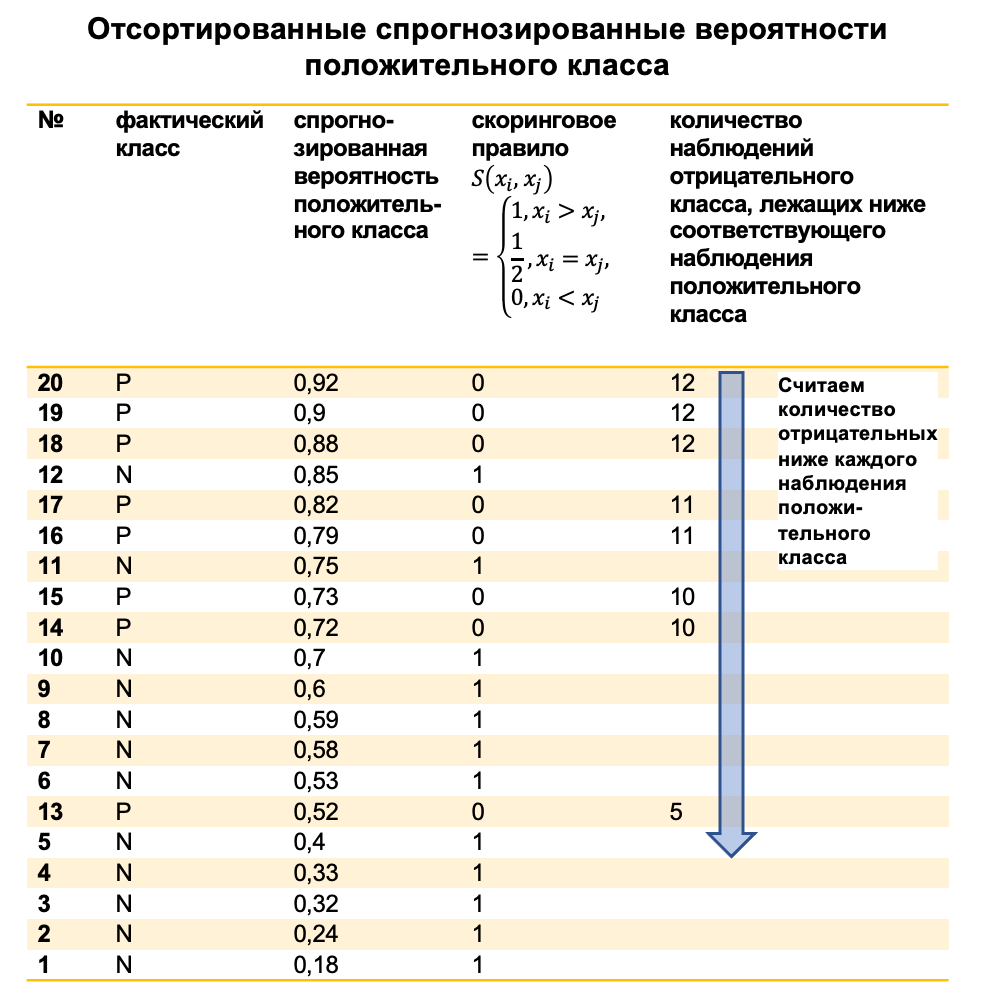
\includegraphics[scale=0.35]{figures/roc_auc1.png}
	\caption{ Расчет ROC-AUC по формуле \eqref{eq:rocauc}}\label{fig:roc_auc1}
\end{figure}

\begin{figure}[h]
	\centering
	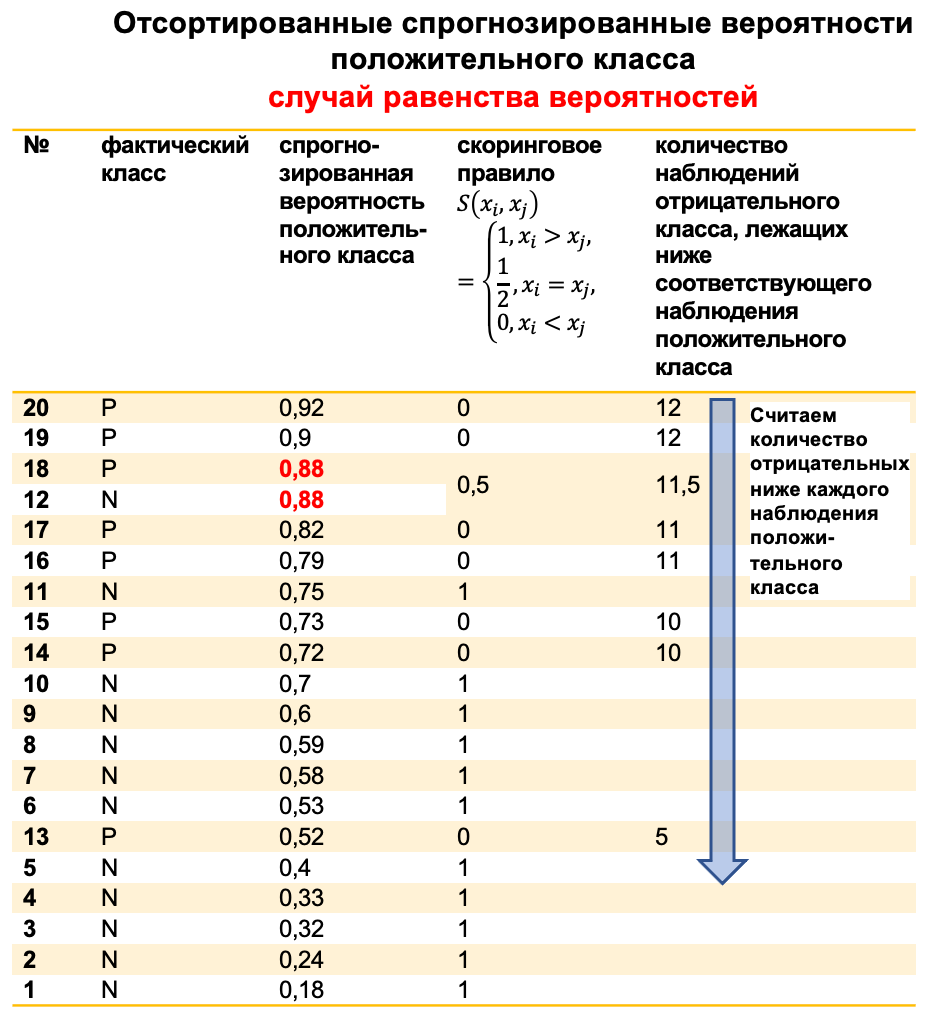
\includegraphics[scale=0.35]{figures/roc_auc2.png}
	\caption{ Расчет ROC-AUC по формуле \eqref{eq:rocauc} для случая равных вероятностей принадлежности экземпляра положительному классу}\label{fig:roc_auc2}
\end{figure}




\listoffigures\addcontentsline{toc}{section}{Список иллюстраций}

% Источники в "Газовой промышленности" нумеруются по мере упоминания 
\begin{thebibliography}{99}\addcontentsline{toc}{section}{Список литературы}
	\bibitem{lutz:learningpython-2011}{\emph{Лутц М.} Изучаем Python, 4-е издание. -- Пер. с англ. -- СПб.: Символ-Плюс, 2011. -- 1280~с. }
	
	\bibitem{geron:hands_on_ml}{\emph{Жерон О.} Прикладное машинное обучение с помощью Scikit-Learn и TensorFlow: концепции, инструменты и техники ля создания интеллектуальных систем. -- СПб.: ООО <<Альфа-книга>>, 2018. -- 688 с.}
	
	\bibitem{burkov:2020}{\emph{Бурков А.} Машинное обучение без лишних слов. -- СПб.: Питер, 2020. -- 192 с.}
		
	\bibitem{beazley:python-2010}{\emph{Бизли Д.} Python. Подробный справочник. -- Пер. с англ. -- СПб.: Символ-Плюс, 2010. -- 864~с. }
\end{thebibliography}

\end{document}
